%\documentclass[journal=jpr,manuscript=article]{achemso}
\documentclass{article}
\usepackage[margin=0.5in]{geometry}
\usepackage{graphicx}
\usepackage{mathtools,amssymb}
%\usepackage{dsfont}
\usepackage{color}
\usepackage[english]{babel}
\usepackage{authblk}
\usepackage{url}
%\usepackage{soul}
\usepackage[ruled,vlined,linesnumbered]{algorithm2e}
\usepackage{algorithmic}
\usepackage[colorlinks,citecolor=blue,linkcolor=blue,bookmarks=false,hypertexnames=true, urlcolor=blue]{hyperref} 

%\graphicspath{{figs/}}  Store figures at the level of the main doc
\newcommand{\argmax}{\text{argmax}}
\newcommand{\todo}[2]{{\color{red} {\bf TODO-#1}: #2}}
\newcommand{\comment}[2]{{\color{blue} {\bf Comment-#1}: #2}}
\newcommand{\correction}[2]{{\color{red} \st{#1} }{\color{red} #2}}
%\newcommand{\correction}[2]{#2}  % Use this to make a document with hiding track changes.

%\usepackage[backend=biber,style=nature,articletitle=false]{biblatex}
%\usepackage[backend=biber,style=nature]{biblatex}
%\addbibresource{bibliography.bib}

%\usepackage[backend=biber]{biblatex}
%\usepackage{natbib}
%\addbibresource{bibliography.bib}
\newcommand{\pe}[0]{\mathrel{{+}{=}}}

\usepackage{setspace}
\doublespacing
%\newcommand*{\DOUBLEBLINDREVIEW}{} %Uncomment to hide author information for double-blind peer review


\author{Andrey Borevsky}
\author{Attila Kertesz-Farkas$\ast$}
\affil{Laboratory on AI for Computational Biology, Faculty of Computer Science, HSE University,  11 Pokrovsky Bvld., Moscow 109028, Russian Federation}
%\email{akerteszfarkas@hse.ru}
%\phone{+7 (499) 152-07-41}

\title{Accurate false discovery rate control in classification problems with valid empirical p-values}
\begin{document}

\maketitle

\begin{abstract}
	The performance of machine learning-based classifiers can significantly degrade in software production due to domain shifts of batch effects that was not considered during training and validation. In this paper, we present a simple to accurately estimate and control the false discovery rate (FDR) on the test data without using class labels which is also robust to domain shifts. Our technique is based on valid, i.e. uniformly distributed, empirical p-values derived from the distribution of the prediction scores of the negative data, i.e. the null-distribution, produced by the classifier. Then, the FDR can be accurately controlled with, for instance, Benjamini-Hochberg protocol or similar ones. Domain shits can be visually detected by comparing the null distributions of the train and test sets with Q-Q plots. In case of domain shift, simply by re-scaling the test null distribution to the train one provides  accurate FDR control. We compared our method with the Learn-Then-Test approach recently developed by Michael Jordan's lab and our experimental results shows that our technique is more robust to data- and class-label distribution shits. 
	
	 
%Artificial Intelligence has been demonstrated as an incredibly useful instrument for a broad range of tasks. One of them — Bioinformatics — proposed fundamentally novel techniques at the intersection of machine learning and statistics. Despite their potential, these methods have not been utilized for more general tasks yet. Accordingly, in our work, we elaborate a drastically new approach called empirical p-values (EPV). Assuming negative training data of classification task to be the null hypothesis distribution, we calculate the corresponding p-values for the test samples. Later, we expand the BH procedure to control FDR, making it possible both to regulate the interrelation of train and test data distributions, as well as to predict new labels based on those already investigated. The major goal is to accurately predict number of accepted discoveries at each level without true labels.


\end{abstract}
\textbf{Key words:} P-values, Empirical P-values, False Discover Rate, Error Control, False Discovery Rate Control, Benjamini-Hochberg Protocol

\section{Introduction}

The performance of machine learning-based classifiers in software production phase is assumed to be the same as its performance on a validation set  \cite{dmlsbook2022}. Unfortunately, the  performance in real world applications can often be significantly worse than thought due to data distribution shift (a.k.a. covariate shift), data label distribution shift, and batch effects \cite{Candela2009DatasetShift} caused by some confounding factors. In life sciences, this shift can be attributed including, but not limited, to change in laboratory or environmental conditions, change in the reagents or atmospheric ozone levels, as well as to personnel differences and to variation of technical sources \cite{leek2010tackling}. Different high-throughput instruments produced by different manufacturers may also produce slightly differently distributed data about the same experiments. Quantitative morphological features of cells from multi-channel fluorescence microscopy images may depend on lamp intensities, filter patterns, dyes \cite{bray2016cell}. Tandem mass spectrometry data are affected by differences in experimental protocols and data acquisition conditions, reagent batches, or changes in instrumentation \cite{phua2022perspectives, vcuklina2021diagnostics}. These impacts may lead to incorrect conclusions about the experiments, and improper clinical drug therapies etc. 

Similarly in economics and industry, machine learning-based predictions may also become inaccurate after economic shock, technological advancement, geopolitical turbulence, and pandemic \cite{ramey2016macroeconomic}. For instance, energy consumption prediction needs to be re-calibrated after energy price change in order maintain carbon emission reasonably low \cite{clement2023coping}; credit risk assessment needs to be adapted to, for instance, monetary policy tightening, increased government expenditure, and income distribution shift caused by inflation \cite{kritzman2012regime,guo2023predict}.
% \cite{Zhang:EECS-2021-262}  % Inflation Reduction Act (IRA)

False positive (FP, aka type I) and false negative (FN, aka type II) errors can have significantly different costs or impacts on people and society \cite{wynants2019three}. For instance, a false positive diagnoses of HIV, COVID-19, and cancer can cause emotional trauma and the person may undergo invasive treatments with undesirable complications and side effects \cite{newman2021rate, salz2010meta, Tosteson2014Consequences, xu2016frequency} until a more elaborated clinical test establishes the correct diagnosis. However; a falsely diagnosed person with infectious disease may lead to a false sense of safety \cite{mouliou2021false}, may put not only their but other peoples' life in danger \cite{woloshin2020false}, an undetected cancer may prolong and hinder treatment \cite{bradley2021interpreting}, misdiagnosed human papillomavirus (HPV) may progress to cancer precursor lesions \cite{macios2022false,pinsky2015principles}. \todo{AB}{We need citations and examples about FP and FN in social sciences, economics, industry and finance}.

%Modern AI applications decision threshold between positive and negative cases should be carefully chosen which not only minimizes the risk of progression of the disease that escaped detection, unfavorable prognosis, and delayed treatment, but also reduces the over-diagnosis, over-treatment, high costs, and needless anxiety .


Modern AI applications not only do they need to increase their discriminative power to reduce the overall number of incorrect predictions, but they also need to simultaneously minimize a quantified risks of false positive and negative errors by an optimal decision threshold calibration while also being able to handle (or detect) data distribution shift \cite{feng2022clinical, al2023artificial}. False discovery rate (FDR) control procedures are plausible techniques to keep the FP rate among the total positive classifications at a certain, user-defined level \cite{Benjamini1995Controlling}, when the risk of FP prediction is significantly higher than cost of FN predictions. The FDR control became popular with the emergence of high-throughput and shotgun experiments which measured large amount of distinct variables simultaneously per sample in a cost efficient way. For instance, microarrays measure the expression levels of thousands of genes simultaneously and FDR control allows to select promising genes for followup studies \cite{storey2002direct,storey2003statistical}. Tandem mass spectrometry can be used to quantify and identify thousands of proteins in a complex biological/chemical sample and FDR control allows to select the trustworthy protein identifications \cite{elias2007target}. Automatic patch clamp systems employ a deep-learning-based image processing module to automatically detect target cells (e.g. nerve cells in living brain) and then it calibrates the movement of a micropipette to approach the cell for future experiments \cite{koos2021automatic}. Cell morphological profiling in high-throughput imaging assays for studying compound libraries and human diseases \cite{moshkov2024learning} relies on automatic cell segmentation and detection often in 3D images \cite{falk2019u}. The FDR control here could curb the error in selecting wrong cells for subsequent experiments and feature quantification. 

The False Selection Rate (FRS) control procedure can restrain the FP and FN errors simultaneously \cite{zhao2023controlling}. This approach determines two thresholds, one to make definitive positive, and another one to make definitive negative predictions. Any samples not passing either thresholds are remain in {\em indecision}. Therefore, the misclassification error (accuracy) among definitive predictions can be bounded, while a subset of samples without predictions are returned for manual investigation by a human expert or for further data collection \cite{rava2021burden}. 

Typically, the FDR (and the FSR) control heavily relies on valid, i.e. uniformly distributed, p-values, while typical deep learning models produce raw discriminative scores, logits for samples. %Recent methods in outlier detection \cite{bates2023testing,marandon2023adaptive} and in classification \cite{rava2021burden, angelopoulos2021learn} have proposed using empirical p-values, also known as conformal p-values, in which a p-value of a given discriminative score $s$ is defined as the fraction of a set of validation  scores that are larger than or equal to $s$, formally: $p=(1+\sum_{s_i\in C} \mathds{1}\{s_i\ge s\})/(n+1)$. 
The empirical p-value (EPV), also known as conformal p-value, of a given discriminative score $s$ is defined as the fraction of a set of validation scores that are greater than or equal to $s$, formally: $p=(1+\sum_{s_i\in H_0} {1}\{s_i \ge s\})/(n+1) \label{eq:epv}$ [eq. \ref{eq:epv}]. The set $H_0$ contains $n$ scores produced by a machine learning method (scoring function) on negative samples of the validation set, which can be constructed from the labeled training data or it can be created from the decoy peptides in tandem mass spectrometry data annotation \cite{elias2007target,danilova2019bias}. The p-values of the negative test samples are super uniform under the null if the data distribution of the test and validation samples are identically and independently distributed. This property is called exchangeability. In this case, the Benjamini-Hochberg (BH) procedure controls the FDR at $\pi_0\alpha$ level, where $\pi_0$ denotes the fraction of nulls (negatives) among the test samples, and $\alpha$ is a user-defined confidence level. The EPVs have been successfully used in recent methods for outlier detection \cite{bates2023testing,marandon2023adaptive} and in classification \cite{rava2021burden, angelopoulos2021learn} under the assumption of exchangeability.   However, in practice, this assumption is often violated due to data shifts, batch effects, as discussed above; thus, the FDR control may be conservatively or liberally (anti-conservatively) biased. 

Recent methods, which deal with data shift, aim to (1) detect data shift  \cite{ dasu2009change}, (2) identify features which cause data shift \cite{kulinski2020feature}, (3) detect and correct label shift \cite{lipton2018detecting}, (4) provide explainability about data shift \cite{budhathoki2021did,kulinski2023towards}, and adapt to data shifts \cite{sui2024unleashing, zhang2021adaptive, zhang2022memo}. Most of the recent methods operate in the feature space and rely on data clustering or graphical cuasel models; and, are challenged by high-dimensional space, data sparsity, and correlated features. 


%These methods usually tackle data shift problems down with (1) data clustering or kernel density estimator algorithms to discover new data clusters, graphical causal models


In this paper we propose a method to adapt the distribution of the scores of negative test samples to the null (i.e. the distribution of the scores of the negative train samples) in order to maintain accurate FDR control under data distribution shift. In detail, the empirical p-values of the test samples are calculated with using the whole negative training data as $H_0$ with eq. \ref{eq:epv}. In the absence of data shift, the p-values should be uniformly distributed. We propose to visually monitor the uniformity of the p-values with Q-Q plots, in which the p-values are plotted against their ordered normalized positions. Any deviation from the diagonal line of the Q-Q plot would indicate data shift. Alternatively, the Fisher's combinatorial test may also be used to test uniformity \cite{fisher1928statistical}. The distribution of the test scores are adjusted so that the mode of the predicted negative test samples fits to the distribution of scores of the negative training samples. \todo{akf-ab}{summarize the method and cite}. Then, the decision threshold can be calibrated with $\pi_0$-BH method directly for the actual test samples so that it controls the FDR at a predefined $\alpha$-level. This approach is also robust to data label shifts because the $pi_0$ estimation automatically considers the actual rate of the classes; therefore adaptation to altered class balances is not required.

 Or approach operates solely at the space of prediction score, which is typically one dimensional for binary classification, or $k$-dimensional for $k$-class classification problems. Therefore, our approach is not hindered by the course-of-dimensionality; moreover, it can be employed with any machine learning model, given that classification is based on discriminative scores; this includes deep neural networks, black box models, with any kind of data such as tabular, text, audio, image, graph data. The only assumption of our method is that the discriminative score distributions resembles to the ones depicted in Figure \ref{fig:illustration}.

\begin{figure}
	\centering
	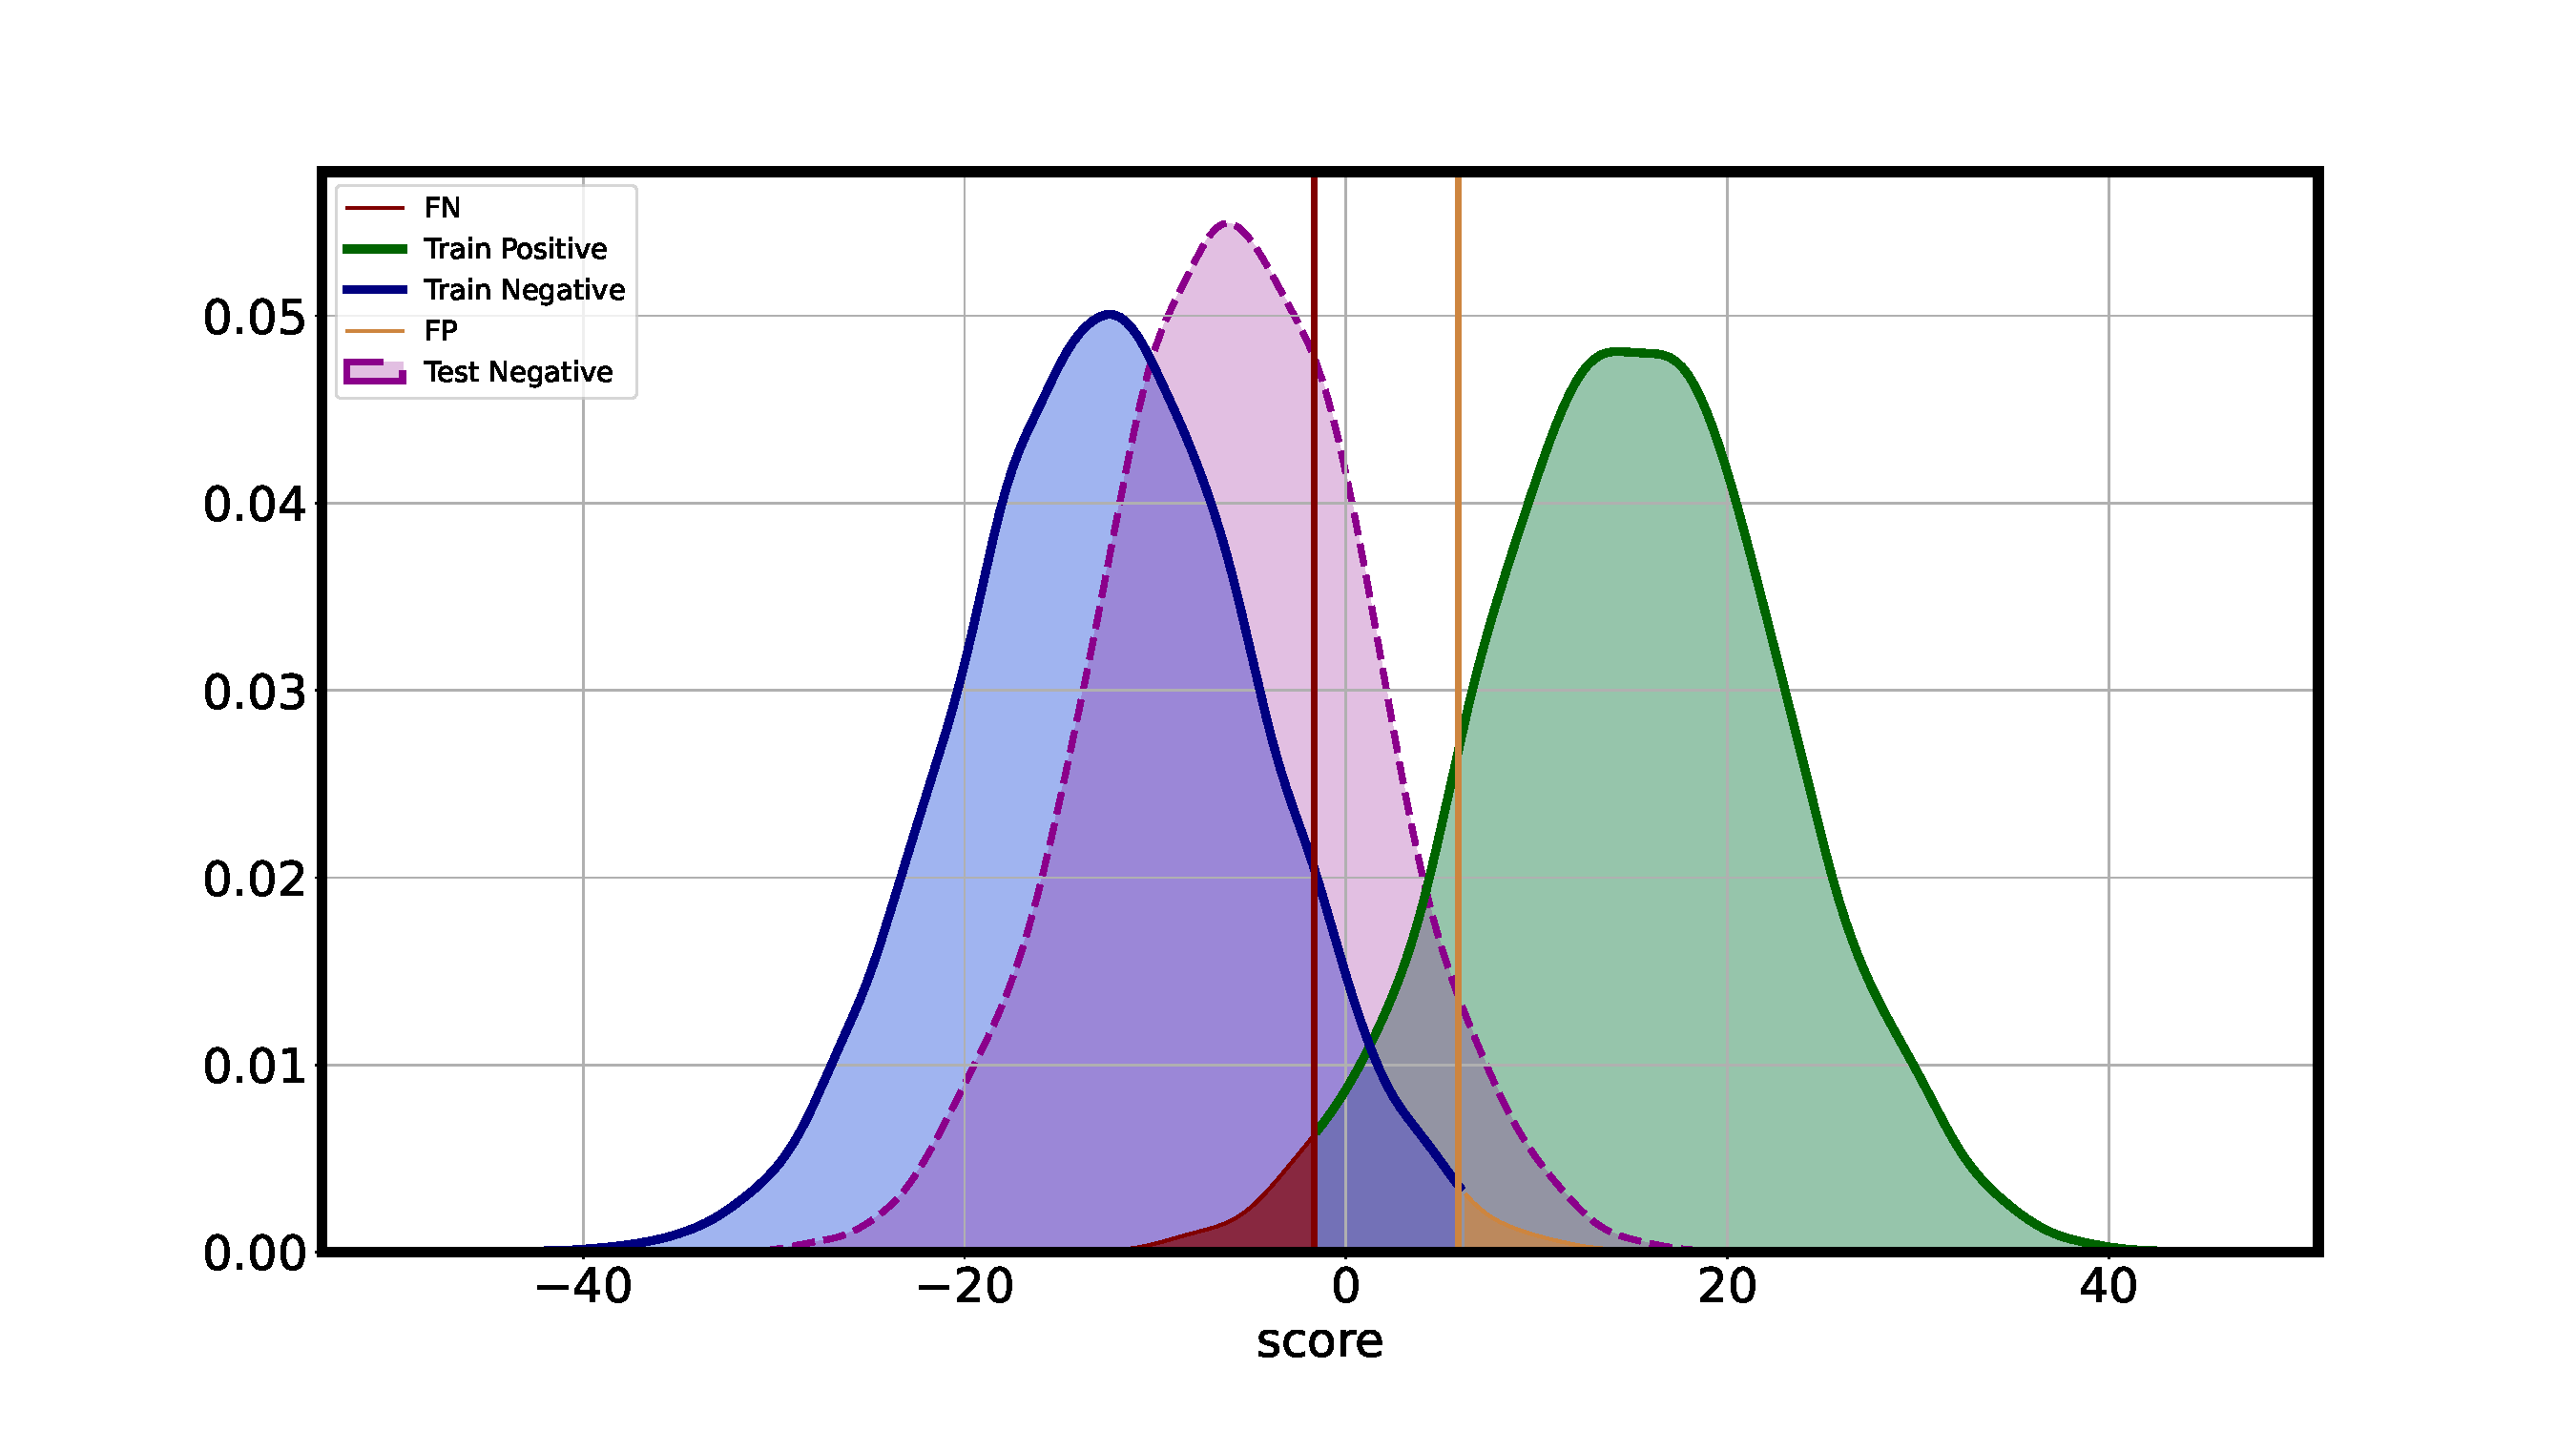
\includegraphics[width=5in]{img/synthetic_overview.pdf}
	\caption{{\bf Error in decision making.} fd}
	\label{fig:illustration}
\end{figure}  




%progression of the disease that escaped detection, unfavorable prognosis, and delayed treatment, but also reduces the over-diagnosis, over-treatment, high costs, and needless anxiety \cite{pinsky2015principles}.

 \

 \
 


Classification is a renown machine learning task, being enriched throughout last decades with various metrics. Each of them expects a growth only with the simultaneous enhancement of the model’s classification power, revealing a certain level of effectiveness. Meanwhile, a broad family of evaluation approaches has been introduced to present a comprehensive analysis. 

Specific cases mandate careful selection of the metric to be used, distinguishing two basic types of errors, which could be made by a classification method. If implying existence of two classes only, then the model might either propose a negative sample to be positive (false negative, FN) or vice versa (false positive, FP). Usually, the type of mistake is indifferent to the inference. However, some situations require diametrically opposite evaluation policy. For instance, we could dive into a biomedical task, such as brain cancer. A neural network processes snapshots of living-patient’s brain cells, searching for those infected. Hence, separating two kinds of error is of paramount importance. Incorrectly recognizing healthy cells as rogue ones (FP) is much more hazardous since the surgeon will remove a wrong part of the brain - action, which can not be undone. Another renown example could be the loan exposure, when a person with a low estimation of credit risk appears to fail to return the debt. So, there is a pool of applications that demand extremely strict control of the extent to which the algorithm makes FP mistakes. In such cases, False Discovery Rate (FDR) seems to be preferable \cite{peaks_de_novo}.

This metric denotes a proportion of samples that belong to type I errors (FP). In other words, this is simply a share of observations, falsely rejecting  $H_0$:

\begin{equation}
            \text{FDR} = \mathbb{E}(V / R \ | \ R > 0) \times \mathbb{P}(R>0)
        \end{equation}
        where V is the number of false discoveries; R is the total number of discoveries \cite{BH}.

Hence, we intend to elaborate a specific approach to produce uniformly distributed p-values of test objects in terms of the negative training data that would further allow to establish certain FDR control policy. Thus, we strive to take statistical methods of bioinformatics and dive into a broader area of ML classification.

Acquiring empirical p-values (EPVs) of test samples towards some null distribution, built from the negatively labeled training data, would allow us to calculate the number of accepted discoveries at each possible error rate without using true labels. Consequently, we will consider identity between rate of FP errors and FDR. However, not only do we want to measure classification results through the FDR metric, but also the latter to be controlled at a certain ground-truth level. Such a task, where an inference strategy should be highly compatible both with the alternative solutions and the ground truth, must consider all potential ramifications of conditions, including data distribution shifts, alterations of class proportions, etc. As a preliminary stage to deduce discoveries at each FDR, it is still vital to approach the uniformly distributed p-values of train data with manually extracted EPVs from test data 

We will hold the synthetic part of the investigation with the convolutional model, processing the MNIST dataset, while later opting to dive into real-life applications. The latter include both a certain range of biomedical application and specific commercial tasks,  specifically, loan exposure risk estimation.

The paper is organized in a classical manner: the introduction is followed by an overview of suggested method with further in-depth exploration of rival  statistical mechanics.  We then dive into the algorithm's embodiment methodology.  Finally, we perform the experiments and consequently depict the outcomes. The entire code can be found in our paper’s \href{https://github.com/Aborevsky01/pvalues_classification}{GitHub repository}.

\section{Concept}

\subsection{FDR-based approach}

In this paper, we propose to put a statistical guarantee with a certain confidence and without any reliance on true labels over the proportion of FP errors, treating it in terms of FDR control. The latter is a family of statistical procedures aimed at formulating a certain $\alpha$ level of FDR metric for a particular number of accepted discoveries. Thereby, we claim to use the negative training data to produce a null distribution $H_0$. In turn, this will allow us to define for a given prediction score $s$ its p-value: 
\begin{equation}
P_{H_0}(s)=\frac{|\{x\mid x>s, x \in H_0\}|}{|H_0|}
\end{equation}
, where $|.|$ denotes the cardinality of set. 

The acquired p-values do allow to establish the FDR control if implementing the Benjamini-Hochberg protocol (BH). It is a ubiquitously recognized step-up technique, elaborated to control FDR at particular $\alpha$ level \cite{BH}. Imagine getting a p-value of 5\% in terms of the constructed $H_0$. Such a result would mean there is only a 5\% chance that a sample belongs to the negative class.  However, sometimes we accidentally discard false positives during our calculations, in turn leading to the higher level of misclassification. As a solution, BH entails first determining p-values by the aforementioned formula. Then, it suggests ordering all p-values in an ascending manner. Next stage is to calculate critical values of each sample by the following formula:
\begin{equation}\label{eq:bh}
    \text{critical value} = \frac{i \cdot \alpha}{m\cdot \pi_0}
\end{equation}
where $i$ is the rank of a p-value;  $\alpha$ is a certain user-defined FDR control level; $m$ is the total number of test samples; $\pi_0$ is the proportion of negative samples in the data, specific correction factor. We need to immediately underscore the fact that no aspect ratio could be available for the test data, if eliminating reliance on true labels. Solution to this issue is later described in the methodology overview. 

As we acquire the BH critical values, it becomes possible to re-establish the particular boundary: the highest rank, so that the corresponding p-value is below its critical value. All the p-values above are considered significant, with a new threshold asserted \cite{qvalues}.

Nevertheless, our key goal is quite different. Instead of moving the border to control FDR at $\alpha$ level, we strive to get an estimation of the latter for each of the possible thresholds. For instance, BH would declare to us how great should be the border of acceptance for credit scores to get an overall FP rate near 10\%. However, we are looking for this very percent of FP at each possible border of acceptance. 

This discourse leads us to the notion of q-values - the adjusted p-values in such a manner that they can be interpreted as FDR. Calculation of those is almost straightly derived from the BH strategy. Firstly, we find $\alpha$ for the particular border in the equation \ref{eq:bh}\footnote{$p_i$ is basically identical to the critical value in the \ref{eq:bh}}. However, range of borders could be represented by the sequence of acquired p-values $p_i$:

\begin{equation}\label{eq:bh2}
    \alpha(p_i) = \alpha_i = \frac{p_i \cdot m \cdot \pi_0}{i}
\end{equation}

The second phase implies finding minimum among all previous p-values in the sorted sequence, which finally gives us q-value for each of the p-values:

    \begin{equation}\label{eq:q}
        \text{q}_{i}(p_{i}) = \min\limits_{t>p_{i}}\alpha(t) \leftrightarrow \min(\alpha_i, \alpha_{i+1})
    \end{equation}

The outcome is the desired estimation of FP rate for some boarder of class division, defined by the previously calculated samples' p-values in terms of negative training distribution. It could and should be visualised via a graph, denoting number of accepted discoveries against the estimated FDR rate. 

At the same time, besides referring to the final inference, we also need an intermediate verification of our method's coherency with reality. Since we propose a practical method excluding the use of true labels and relying on the particular model's accuracy, there is a need to understand how close are our predictions to the reality. At the same time, it is a known fact that if sampling from a distribution, the resulting p-values will be uniformly distributed. \todo{attila}{pls check this part}\textit{Let us assume we are given a continuous, cumulative distribution function $F_X(X)$ and it is invertible, i.e. $F_X^{-1}$ exists. We want to show that the p-values $Z = 1-F_X(X)$ are uniformly distributed, that is $F_Z(X)$ is uniformly distributed. Note that $Z\in [0,1]$. For the uniform distribution on $U\sim U_{[0,1]}$, we also have $1-U\sim U_{[0,1]}$ uniformly distributed, furthermore $P(U\le u)=u$ and $P(U>u) = 1-u$ for any $u\in[0,1]$. Thus,}
\begin{equation}
	F_Z(u)=P(Z \le u) = P(1-F_X(X)\le u)= 1-P(X\le F_X^{-1}(u))=1-F_X(F_X^{-1}(u))=1-u.
\end{equation}

Hence, a bias assessment is opted to be carried out by drawing a QQ plot of the acquired p-values against the theoretical uniform distribution for visual verification.

The described above algorithm seems to be a reasonable strategy to estimate $\alpha$ level of FP at each particular threshold. Nevertheless, the major issue with such a straightforward approach is a colossal reliance on the heuristics, describing the training scores distribution. The consequence appears to be its negligible robustness and adaptation to the class distribution nor to the data distribution shifts. Thus, the method we propose here 
encapsulates the explored concept together with embodying specific rules to counter the alterations of test data.

\subsection{Learn-then-test}

Obviously, FDR is just a single example of the statistical guarantees we can address to the algorithm. An attempt to establish a unified approach for calibrating models to satisfy such explicit constraints was accomplished by \cite{ltt}. Their two-stage Learn-then-Test (LTT) framework proposes acquiring a trained model and modifying its predictions through multiple hypothesis testing. Thus, the acceptable set of hyperparameters is determined to preserve any selected statistical error (including FDR). “\textit{Put plainly, we learn a base model and then test which parameter values lead to risk control}” \cite{ltt}. 

In the FDR case, we are simply searching for an optimal threshold $t$ to be chosen for each desired metric value. Such a strategy, being an extensive way to calibrate the error rate, introduces a brand new technique that will be used as a direct competitor to the introduced method. Speaking more formally, we can take some threshold $t$. Then, we could say that the corresponding classification function $f_t$ (basically, our neural network) is producing $(\alpha, \beta)$-risk-controlling predictions only if:

\begin{equation}
        \mathbb{P}(\mathcal{R}(\mathcal{T}_{\hat{\lambda}}(X)) \leq \alpha) \geq 1 - \beta
\end{equation}
where $\alpha$ and $\beta$ are particular hyperparameters of risk control; $R$ is the risk function, taking as input the prediction set for the particular t. In our case it is mainly the expectation of loss function. 

We find it essential to dive into the underlying mechanism of the embodied algorithm.
\begin{enumerate}%[label=\arabic*.]
    \item As the first step, a sequence of the FDR values for each train sample is generated. We then present a set of possible thresholds in a form of linear space with $k=300$ samples evenly distributed across the entire training array. Consequently, the selected $t$ give us a set of corresponding FDR values from the sequence - risk function $\mathcal{R}$.
    \item Then, we get into a cycle, iterating over possible $\alpha$ values (identical to the estimated FDR level). 
    \item At each step, Hoeffding-Bentkus inequality p-value is estimated. Such a parameter equals minimum of two separate statistical heuristics, both using $\alpha$ and $\mathcal{R}$. The presented by authors formula was proven to offer highly efficient results, formulating the p-value $p_j^{HB}$ for the null hypothesis $\mathcal{H}_j: \ \mathcal{R}(f_t) > \alpha$. "\textit{A small p-value will indicate disagreement with $\mathcal{H}_j$, implying the risk is controlled.}" \cite{ltt}
    \item The second key stage of the LTT framework assumes multiple hypothesis testing through the Bonferonni correction. It allows to reject all the thresholds out of those selected earlier based on the inferred p-values, limiting the false rejection probability for the given $\beta$-level. Out of the preserved hypothesis the last is chosen.
    \item After the best threshold-score was selected, we can measure percentage of test scores above it. Consequently, calculating such a share for the test data, we can not only separate distribution into positive and negative subsets, but also identify particular number of accepted discoveries at particular $\alpha$.
\end{enumerate}

\section{Empirical P-Values}

\subsection{Methodology}
After a number of various permutations, each being scrutinized for the sake of higher efficiency, a particular approach was elaborated. It includes the following stages:


\begin{enumerate}%[label=\arabic*.]
    \item The neural network is trained in a classic manner on training data $X^{\text{train}}$, regardless of the classification type (binary or multiclass).
    \item Trained model is switched to the inference mode. Particular scores are then divided into the positive training data $P^{\text{train}}$, negative training data $N^{\text{train}}$ and the entire test dataset $X^{\text{test}}$.
    
    \item $X^{\text{test}}$ is generalized and statistically adjusted in order to prevent issues with data distribution / class balance shifts, acquiring in result the $\hat{X}^{\text{test}}$. It is in-depth explored further in \ref{StatAd}.

    \item  After we acquired the modified test distributions, we stack them together: $\hat{X}^{\text{test}} = [\hat{P}^{\text{test}}, \hat{N}^{\text{test}}]$. Deriving our final data representation allows to launch statistical algorithm on competing approaches, either including or eliminating statical adjustment of test data.

    \item The empirical p-values extraction incorporates several stages. \begin{itemize}
        \item  Firstly, we calculate such p-values that reflect the position of the particular test sample according to the $N^{\text{train}}$:

    \begin{equation}
        \text{p}_i = \frac{L_{N^{\text{train}}} - \text{position}(N^\text{train}, \hat{X}^{\text{test}}_i)}{L_{N^{\text{train}}}}
    \end{equation}
    where $L_{N^{\text{train}}}$ is the total number of samples in $\hat{N}^{\text{train}}$; position is the output of binary search algorithm, declaring sample's $\hat{X}^{\text{test}}_i)$ position in the sequence $N^{\text{train}}$. 

    \item Next, the sorted sequence of EPVs is returned to become an input for the BH procedure. There, we deduce the corresponding q-values by the formula\ref{eq:bh2}. It requires the ratio of the positive (null hypothesis) and the negative (alternative hypothesis) classifications. Such a value is denoted as $\pi_0$. In our case, $\pi_0$ is estimated by the share of those samples predicted to be negative among the entire test dataset. 
    \item Final operation implies the same procedure, as shown in equation\ref{eq:q}.
    \item The extent of algorithm's predictions' correctness is assessed through the verification procedure. After the entire method has culminated, we can calculate the deviation of estimated EPVs from the perfect diagonal, being visualized on the QQ plots. 
    \end{itemize}
\end{enumerate}

\subsection{Statistical adjustment}\label{StatAd}

\subsubsection{Distribution shift disposal}

Alterations among the test samples compared to the training ones are a well-known issue. Therefore, the established method should demonstrate resilience by maintaining the quality of predictions. This is achieved through a multi-stage algorithm.

Firstly, we apply the kernel density estimation separately to the $P^{\text{test}}$ and $N^{\text{test}}$ subsets, which are initially split according to the given threshold. Next, we extrapolate both resulting functions and determine the two lines' point of intersection to be the novel, slightly displaced border. This deviation from the standard methodology was implemented to address potential challenges caused by shifts in data distribution, wreaking havoc in estimations. Additionally, this technique enables the approximation of hidden tails, which can significantly affect overall performance. 

The mean and standard deviation of both $P^{\text{train}}_{\text{true}}$ and $N^{\text{train}}_{\text{true}}$ are then calculated to describe them based on their true labels, which the model initially learned from. We then substitute $\mu^{\text{test}}_N$ and $\sigma^{\text{test}}_N$ by the training ones. In the case of a positive subset, only $\mu^{\text{test}}_P$ is modified.
    \begin{equation}
            \hat{N}^{\text{test}} = \frac{(N^{\text{test}} - \mu^{\text{test}}_N)}{\sigma^{\text{test}}_N} \cdot \sigma^{\text{train}}_{N_{\text{true}}} + \mu^{\text{train}}_N{\text{true}}
    \end{equation}
The changes listed bring the test data closer to the training data, resulting in greater uniformity  of $\hat{N}^{\text{test}}$ EPVs.



\subsubsection{Tail Approximation}

As the study focuses primarily on the FP notion, it is crucial to acknowledge the presence of tails in test distributions. While we do not have access to the labels, we cannot accurately prolongate either $\hat{P}^{\text{test}}$ or $ \hat{N}^{\text{test}}$. However, we have information not only on the correct training distribution - $P^{\text{train}}_{\text{true}}$ and $N^{\text{train}}_{\text{true}}$ -, but also on the transformation towards the predicted case. To clarify, the latter is when training values are split based only on model's prediction: $P^{\text{train}}_{\text{pred}}$ and $N^{\text{train}}_{\text{pred}}$. 

After  the difference between the shapes of the train and test subsets, we can now perform the following strategy. Initially, we consider $p^{\text{train}}_{b}$ to be the rightwards p-value of the updated classification's threshold value in terms of $\hat{N}^{\text{test}}_{\text{true}}$. Next, we take the identical leftwards p-value of the negative test distribution $ \hat{N}^{\text{test}}$, striving to create a symmetric plot.Our next step is to concatenate the left-side tail, starting from $-p^{\text{train}}_{b}$, to the right side of the negative test distribution. Reversing the tail while keeping the relative proportions is not a significant issue. However, it seems that after making rough estimate of the tail, opting to name $ \hat{N}^{\text{test}}$ and $N^{\text{train}}_{\text{pred}}$ similar, we extended our test data with synthetic samples. This might result a vast range of negative consequences. 

To address this issue, we have elaborated a specific technique. We apply a binning technique for the values within the range of the synthetic tail. Next, we calculate the proportion of those values sampled and reversed from $ \hat{N}^{\text{test}}$ left side in relation to the real data from $P^{\text{train}}_{\text{pred}}$. Thus, we acquire the probability of changing the label of real positively predicted training data for each bin. Such an algorithm allows for the maintainance of only real samples in data, while also predicting the tail of the $ \hat{N}^{\text{test}}$. The same procedure can be performed for $ \hat{P}^{\text{test}}$.

\section{Experiments}
\subsection{Synthetic data}

\subsubsection{Dataset and Model}

In the preliminary part we are working solely on the ubiquitously known MNIST dataset, a rich collection of handwritten digits, becoming a baseline for any classification task nowadays. It contains 60k samples for the training stage and only 10k for the test, where all classes (from 0 to 9) are evenly distributed. Also to be mentioned is the strict normalization of the digits in the image in terms of size and centering, so the algorithms receive unified examples as input.

We have accomplished all our experiments through a standard convolutional neural network \cite{cnn}. It generally comprises two convolutional 2d layers, both with 8 channels, kernels of size 3 and two-step strides. Single rectifier activation function is following each of them.  The output layer is represented by a simple linear unit, providing as much classes, as it was initialized by the user.   

Model is trained with Adam optimizer with a learning rate equal to 0.01 and a BCEWithLogitsLoss cost function unless otherwise specified. The motivation for introducing such a naive model was straightforward: if we find ourselves able to ameliorate a particular quality compared to the ground truth via an elementary model on the resolvable MNIST dataset, then we could extend our approach to more comprehensive real-life tasks and models.

The entire algorithm was written on the PyTorch framework and includes several key stages throughout all separate local experiments. If formalizing our goal, then we could express our dataset as $(X_i, Y_i)_{i\in\{1, ..., n\}}$, where $X_i \in \mathbb{X}$ is a feature vector and  $Y_i \in \mathbb{Y}$ is the labels. For instance, $\mathbb{X}$ can be images and $\mathbb{Y}$ - the corresponding classes. Thus, our machine learning model becomes in some sense a comprehensive function $f$, such that $f(\mathbb{X}): \  \mathbb{X} \rightarrow \mathbb{Y}$.

However, besides only generating uniform p-values, we need an understanding of the algorithm’s efficiency. Thus, we introduce two types of graphs: the “QQ” plots and the “FDR control” plots. The former depicts p-values from the uniform distribution for visual verification. We plot these p-values obtained with negative training data and their rank along the x-axis for both training (simply a diagonal) and test data. The closer our test samples get to the ideal line, the better our EPV approach operates. The second type of graphs visualizes the number of trusted classifications depending on the FDR when it is controlled with true labels (baseline) and with the BH protocol using the p-values. We also add rival LTT framework, representing the FWER methodology. As we progress towards the ground truth, our ability to function without test labels will improve as well as our capacity to forecast. The last paragraph remains true for the further experiments.

\begin{figure}
        \advance\leftskip-0.5cm
	\begin{tabular}{ccc}
 		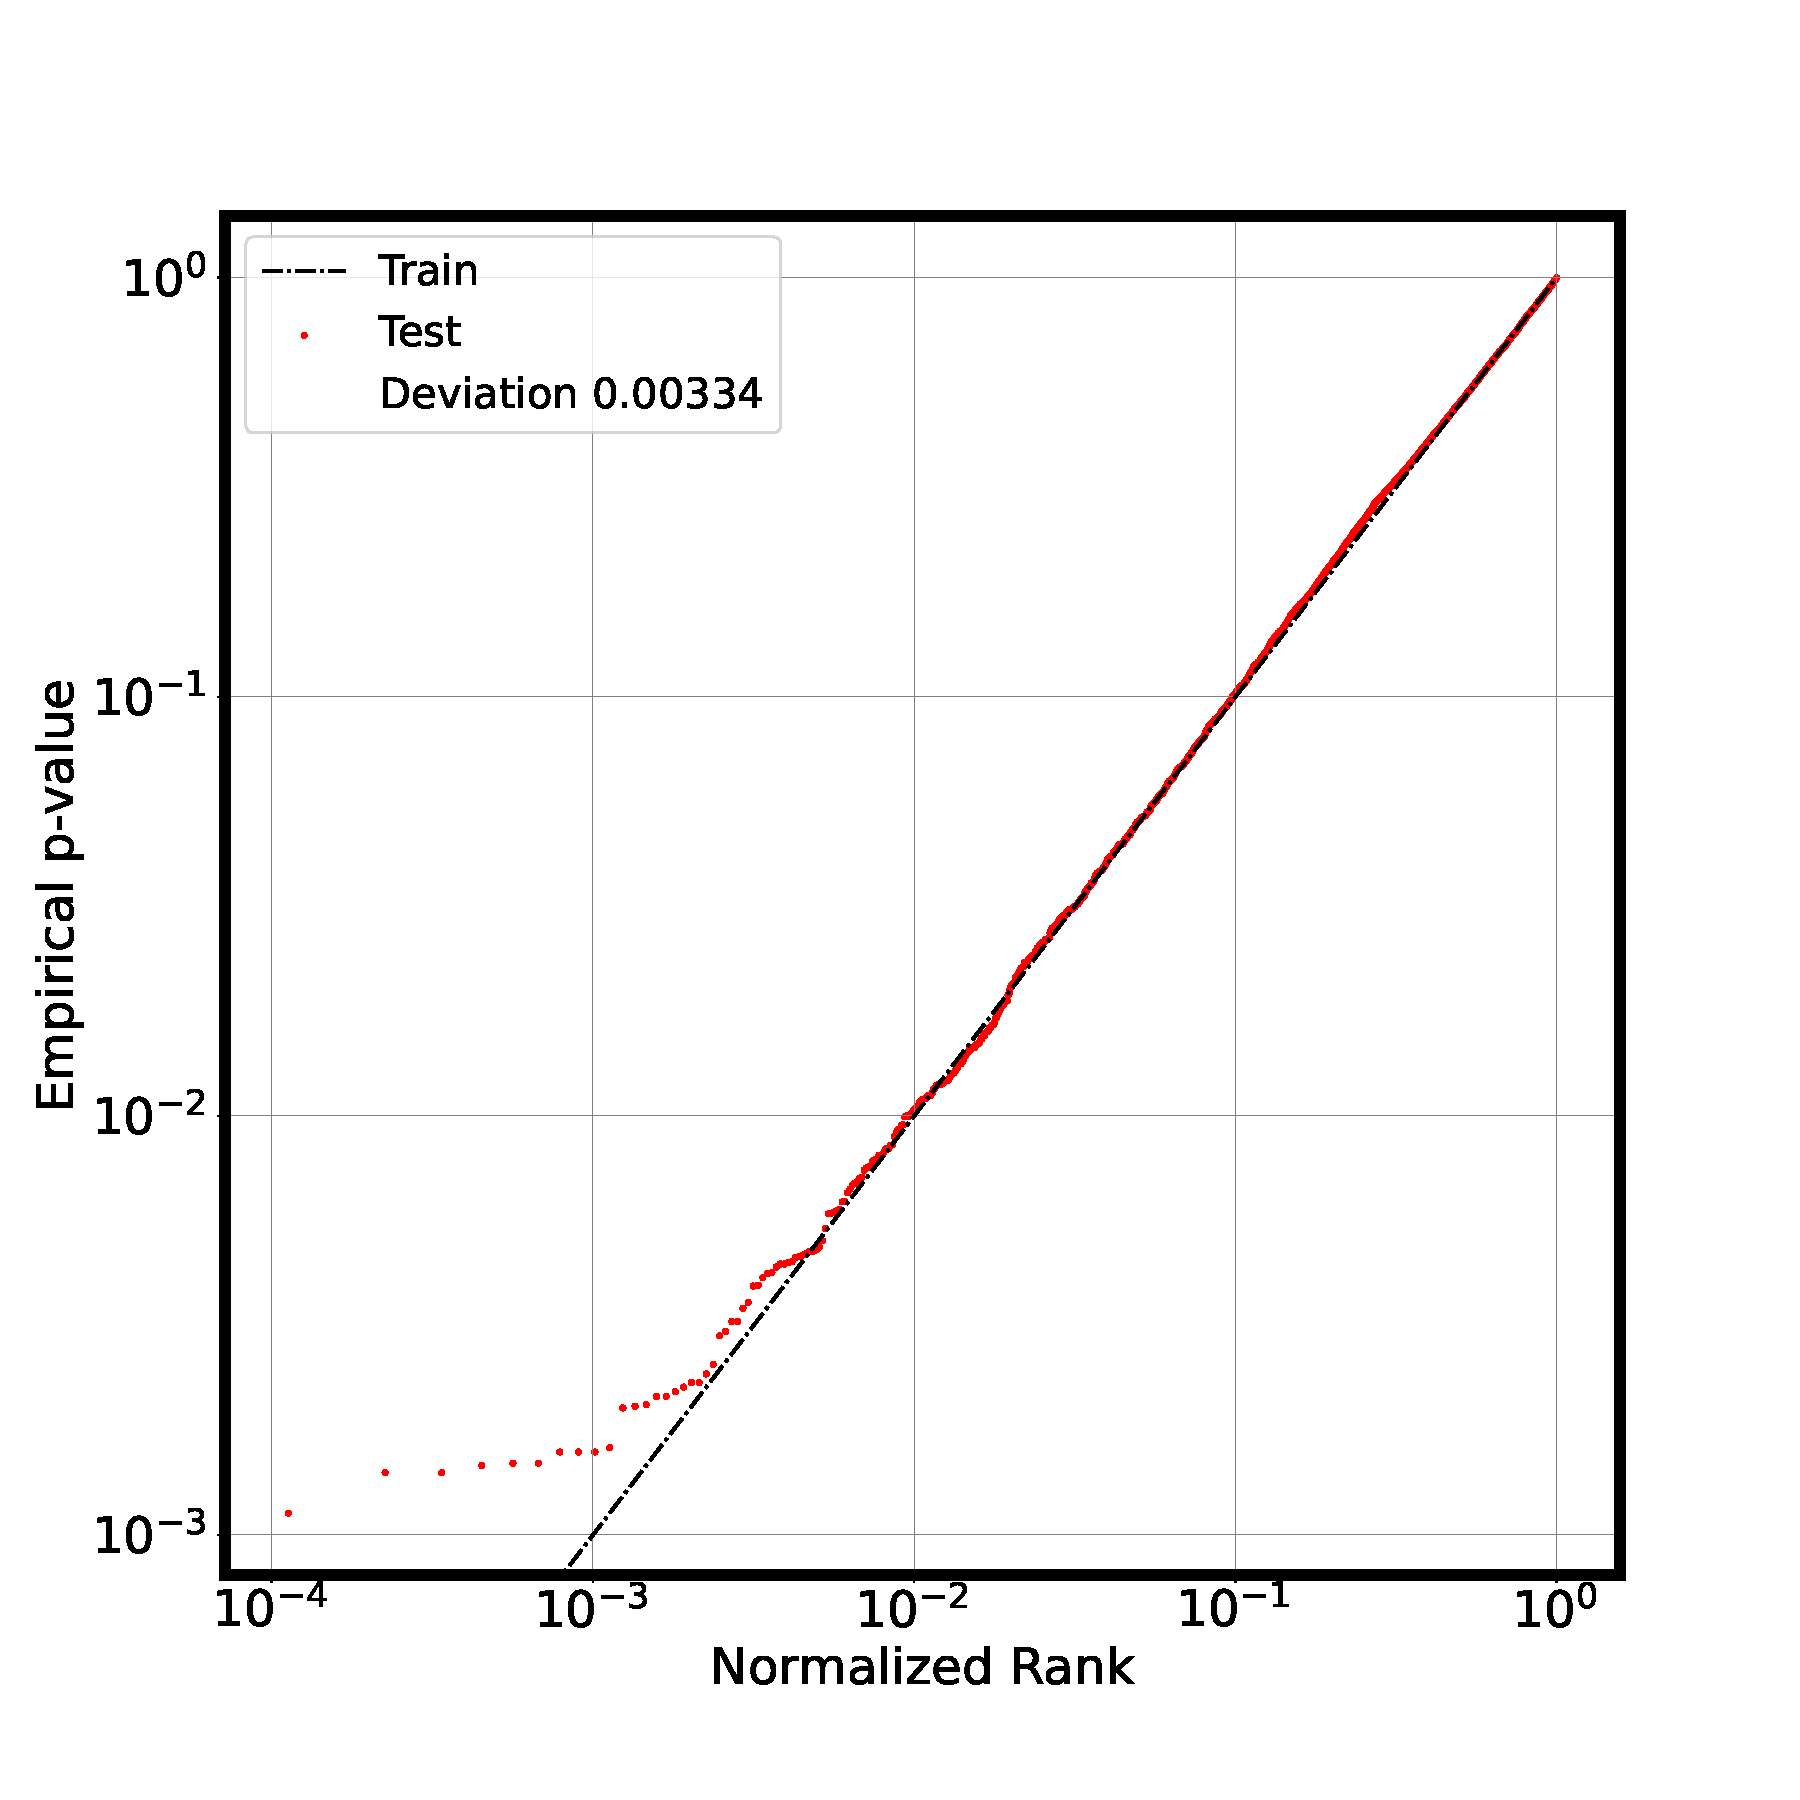
\includegraphics[width=2.5in]{img/cnn_QQ_classical.pdf} &
		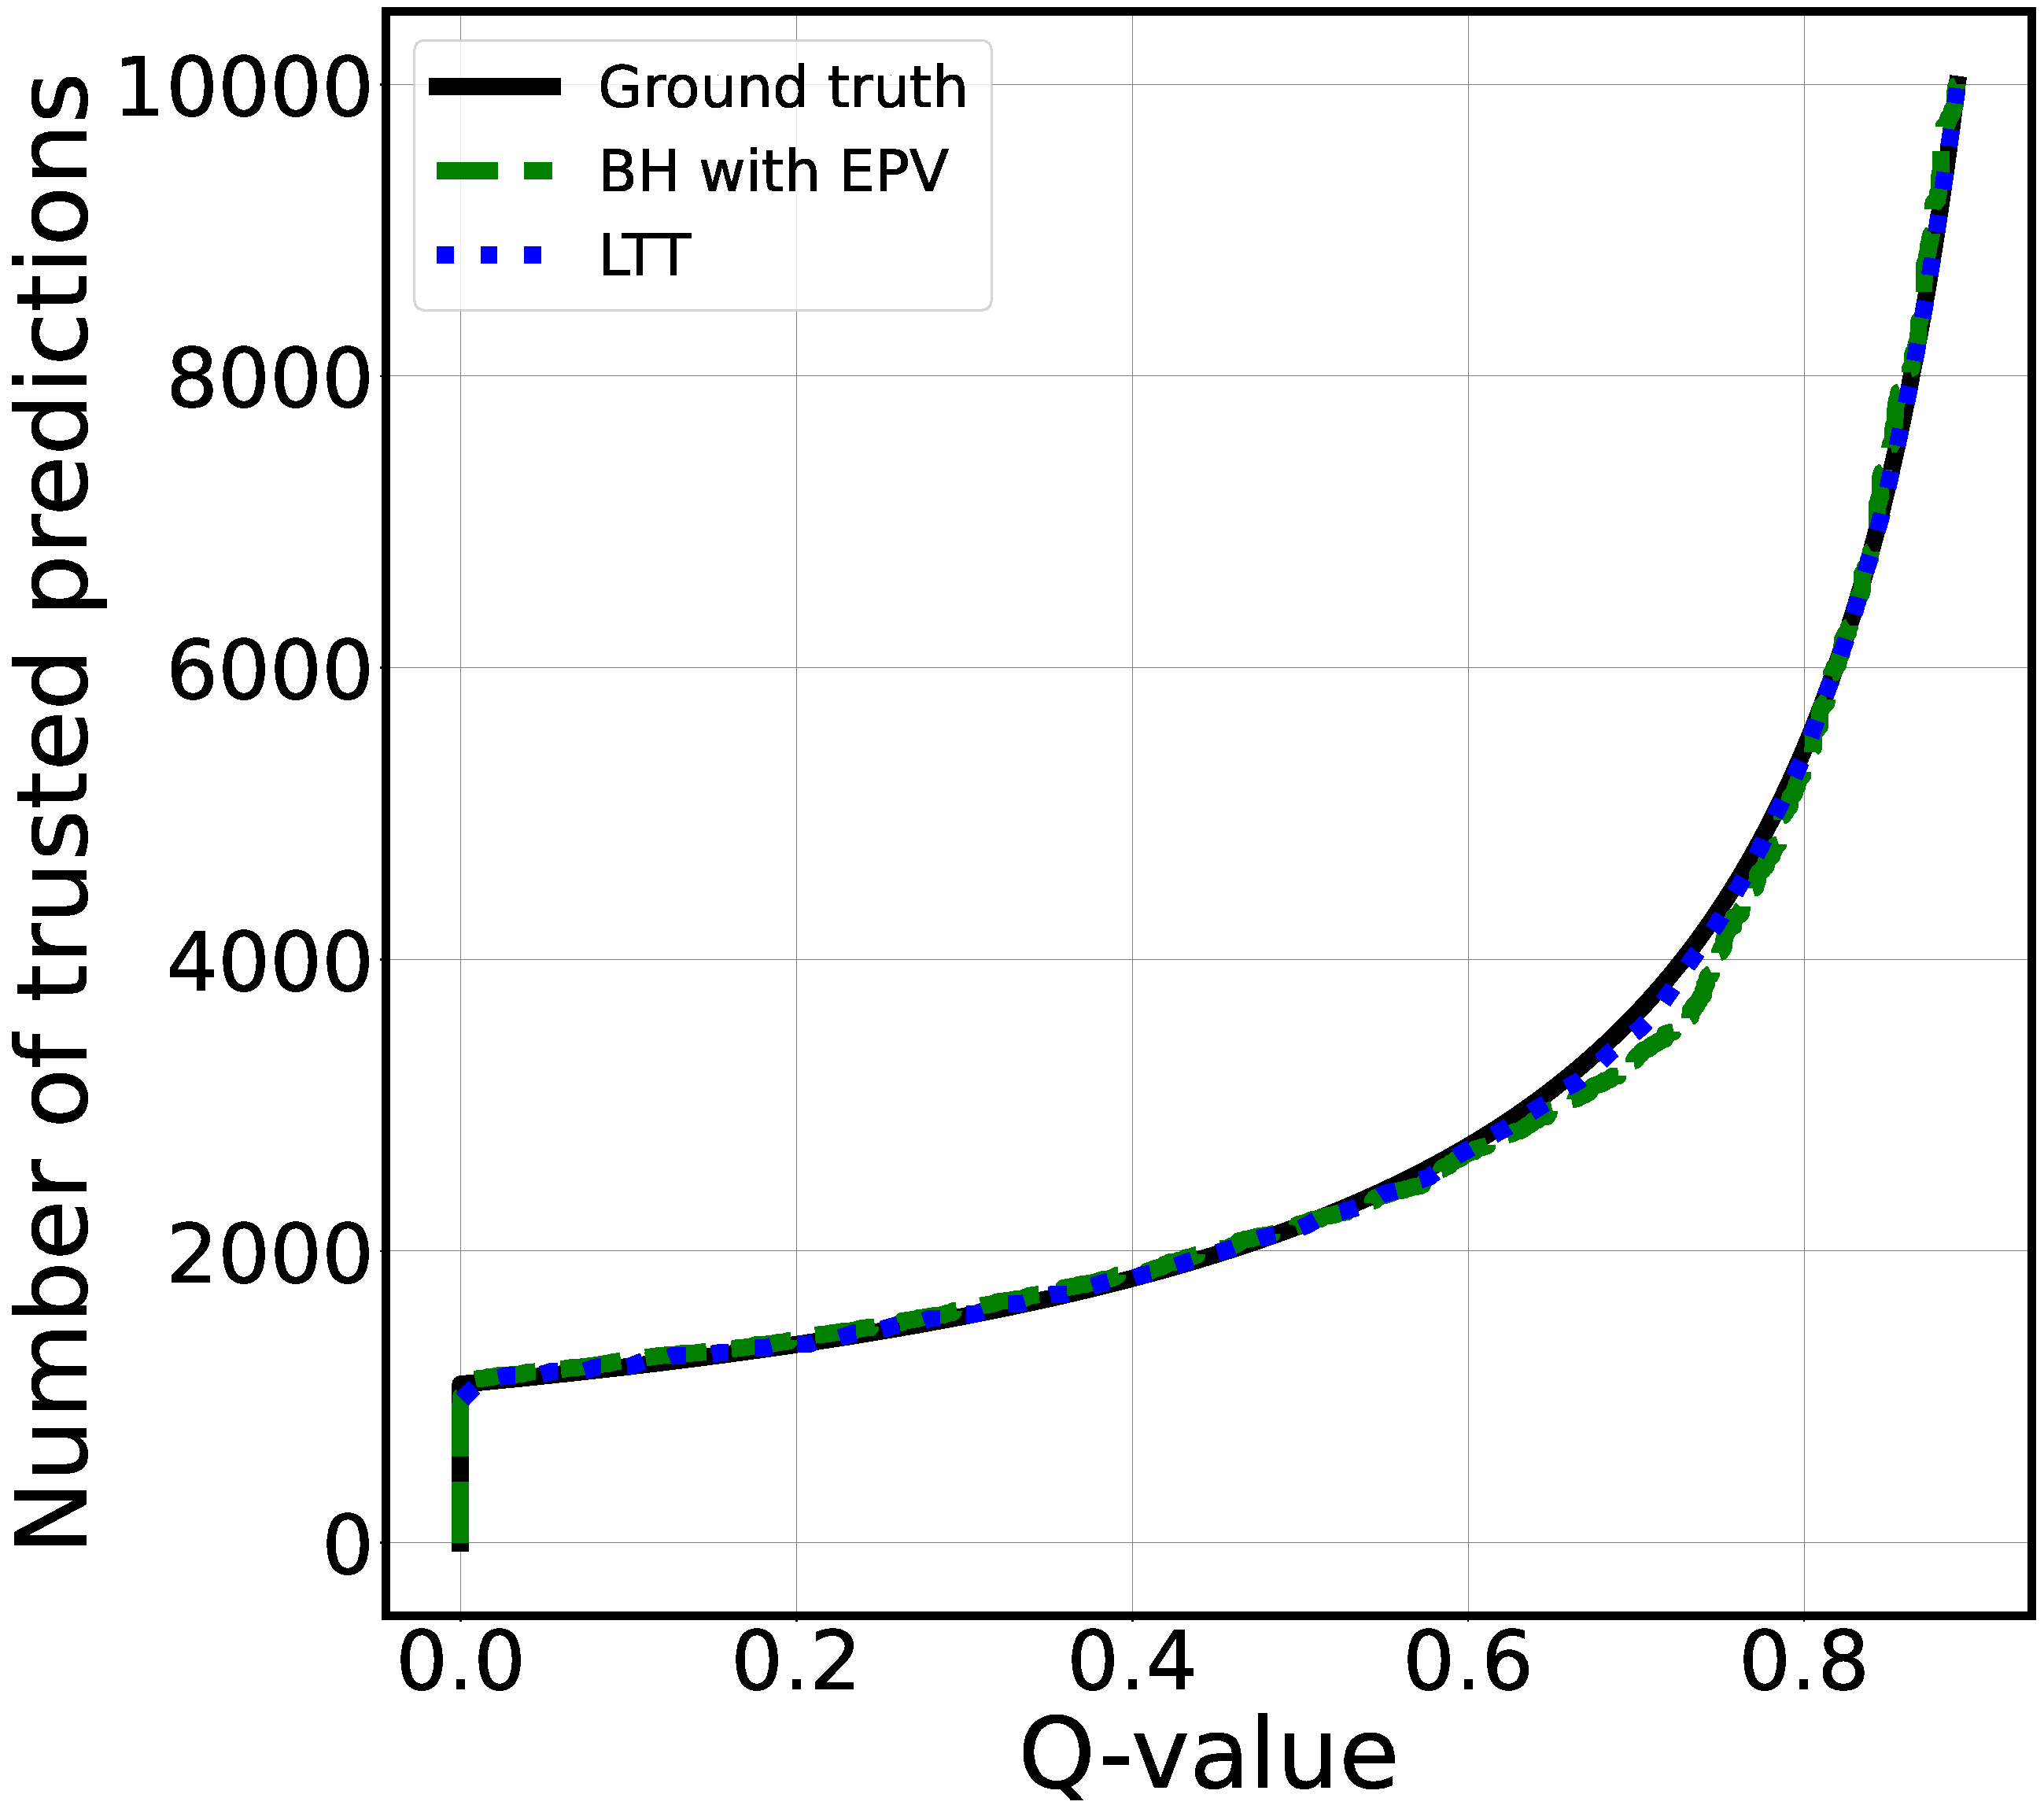
\includegraphics[width=2.5in]{img/cnn_classical_fdr_control.pdf} & 
            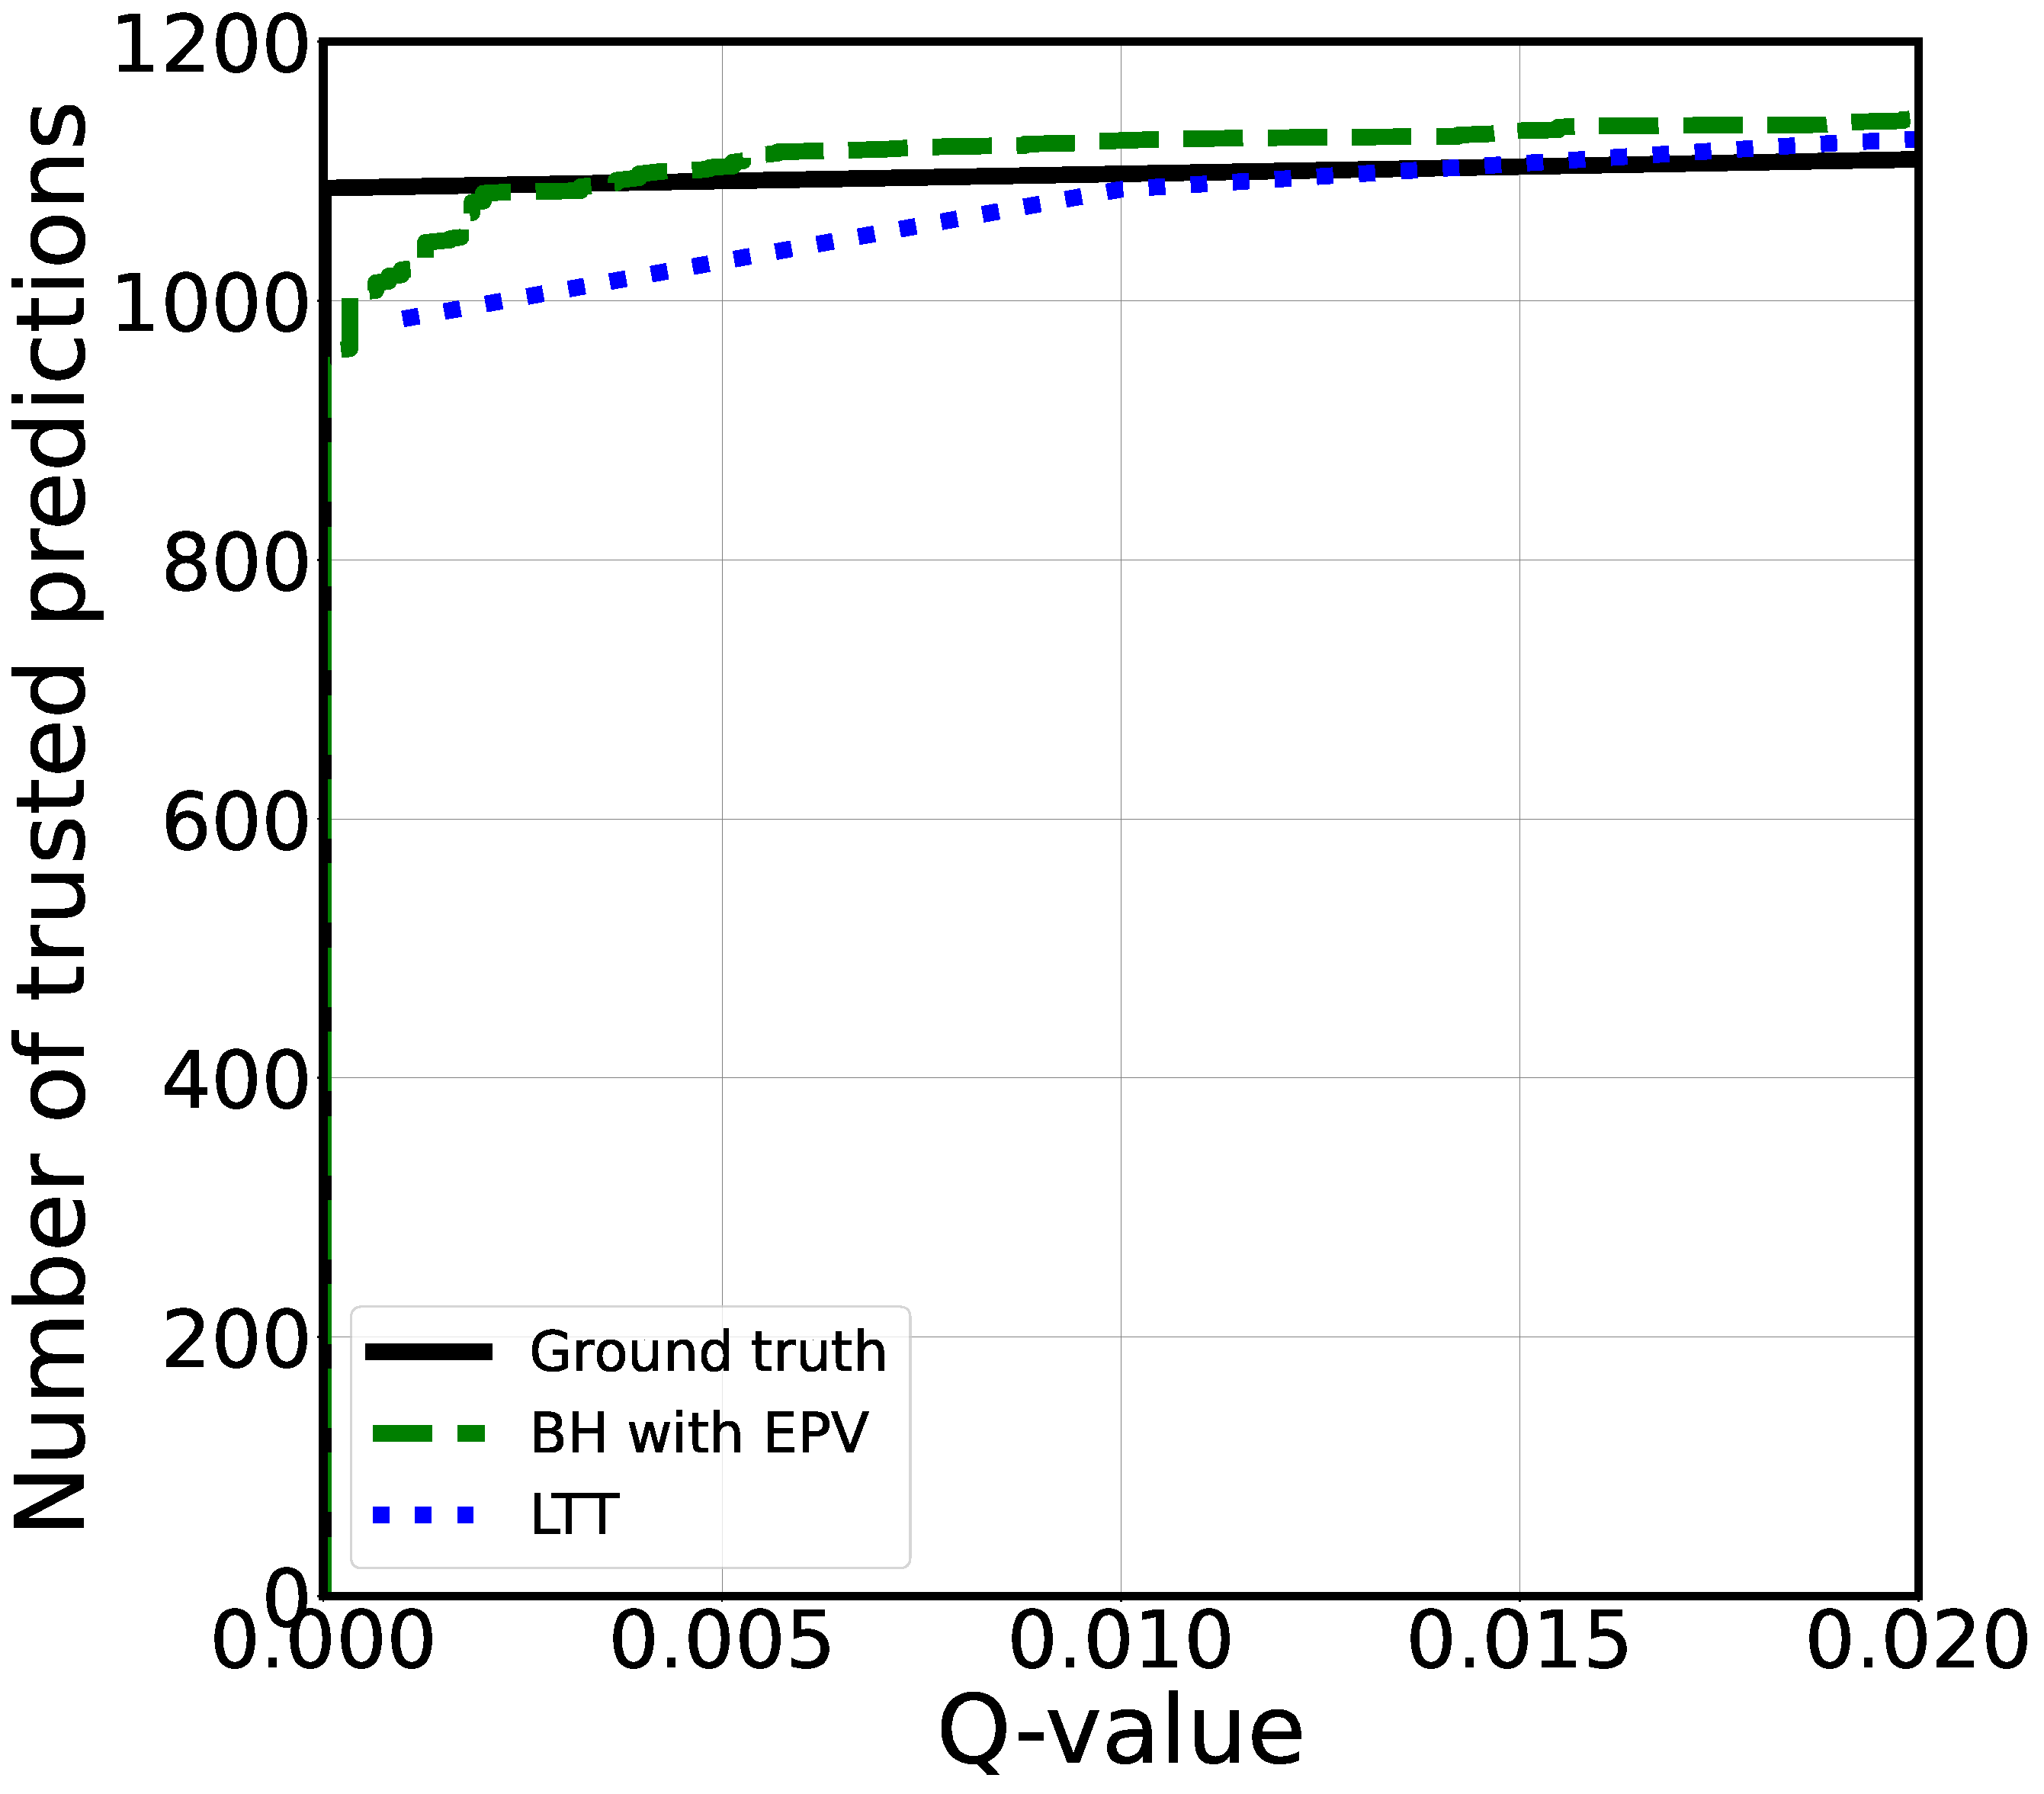
\includegraphics[width=2.5in]{img/cnn_classical_fdr_control_loc.pdf}
		\\
		%    \includegraphics[width=3in]{digestion.pdf} & \includegraphics[width=3in]{cleavages.pdf} \\		
		A & B & C
	\end{tabular}
	\caption{{\bf FDR control with p-values.}
		(A) a QQ plot of the p-values obtained with using negative training data. (B) The number of trusted classifications as a function of the FDR when it is controlled with true labels (red line) and with controlled with BHP (black line) using the p-values from panel (A). $\pi_0$ is estimated on the test data.
		(A) a QQ plot of the p-values obtained with using training data classified as negative. (B) The same as panel (B), but using p-values from panel (C).
	}
	\label{fig:classical}
\end{figure}  

\subsubsection{Binary Case}

Binary classification is a basic task, where $\mathbb{Y} \in {0, 1}$. Hence, both training and test sets can be easily divided into negative and positive shares. Speaking of the MNIST dataset, we get 10\% for positive class despite our choice for the positive class, not playing any crucial role for our research. We arbitrarily chose the class "2" as a positive class from the MNIST data, and all other data corresponding to other classes were treated as negative data. 

As the model was trained, one can use the prediction scores for negative training data as a null distribution. Consequently, we have a zero hypothesis, giving us the probability of test item to either belong to negative class or not. However, the BH protocol requires
the ratio of the positive (null hypothesis) and the negative (alternative hypothesis) classifications. Such a value is denoted as $\pi_0$. In our case, $\pi_0$ is estimated by the share of those samples predicted to be negative among the entire test dataset.  

Speaking of the QQ plots, one almost can not identify any distinctions between perfect diagonal, corresponding to training p-values, and a scatterplot of empirical p-values. Another proof of EPV's high-performance for binary case is the second group of graphs, indicating the correlation of made discoveries' quantity to the proposed FDR. The ground truth seems to be mostly descriable by our method, having a little edge over the LTT method. It is especially visible on a more critical local scale.


\begin{figure}
    \centering
	\begin{tabular}{cc}
		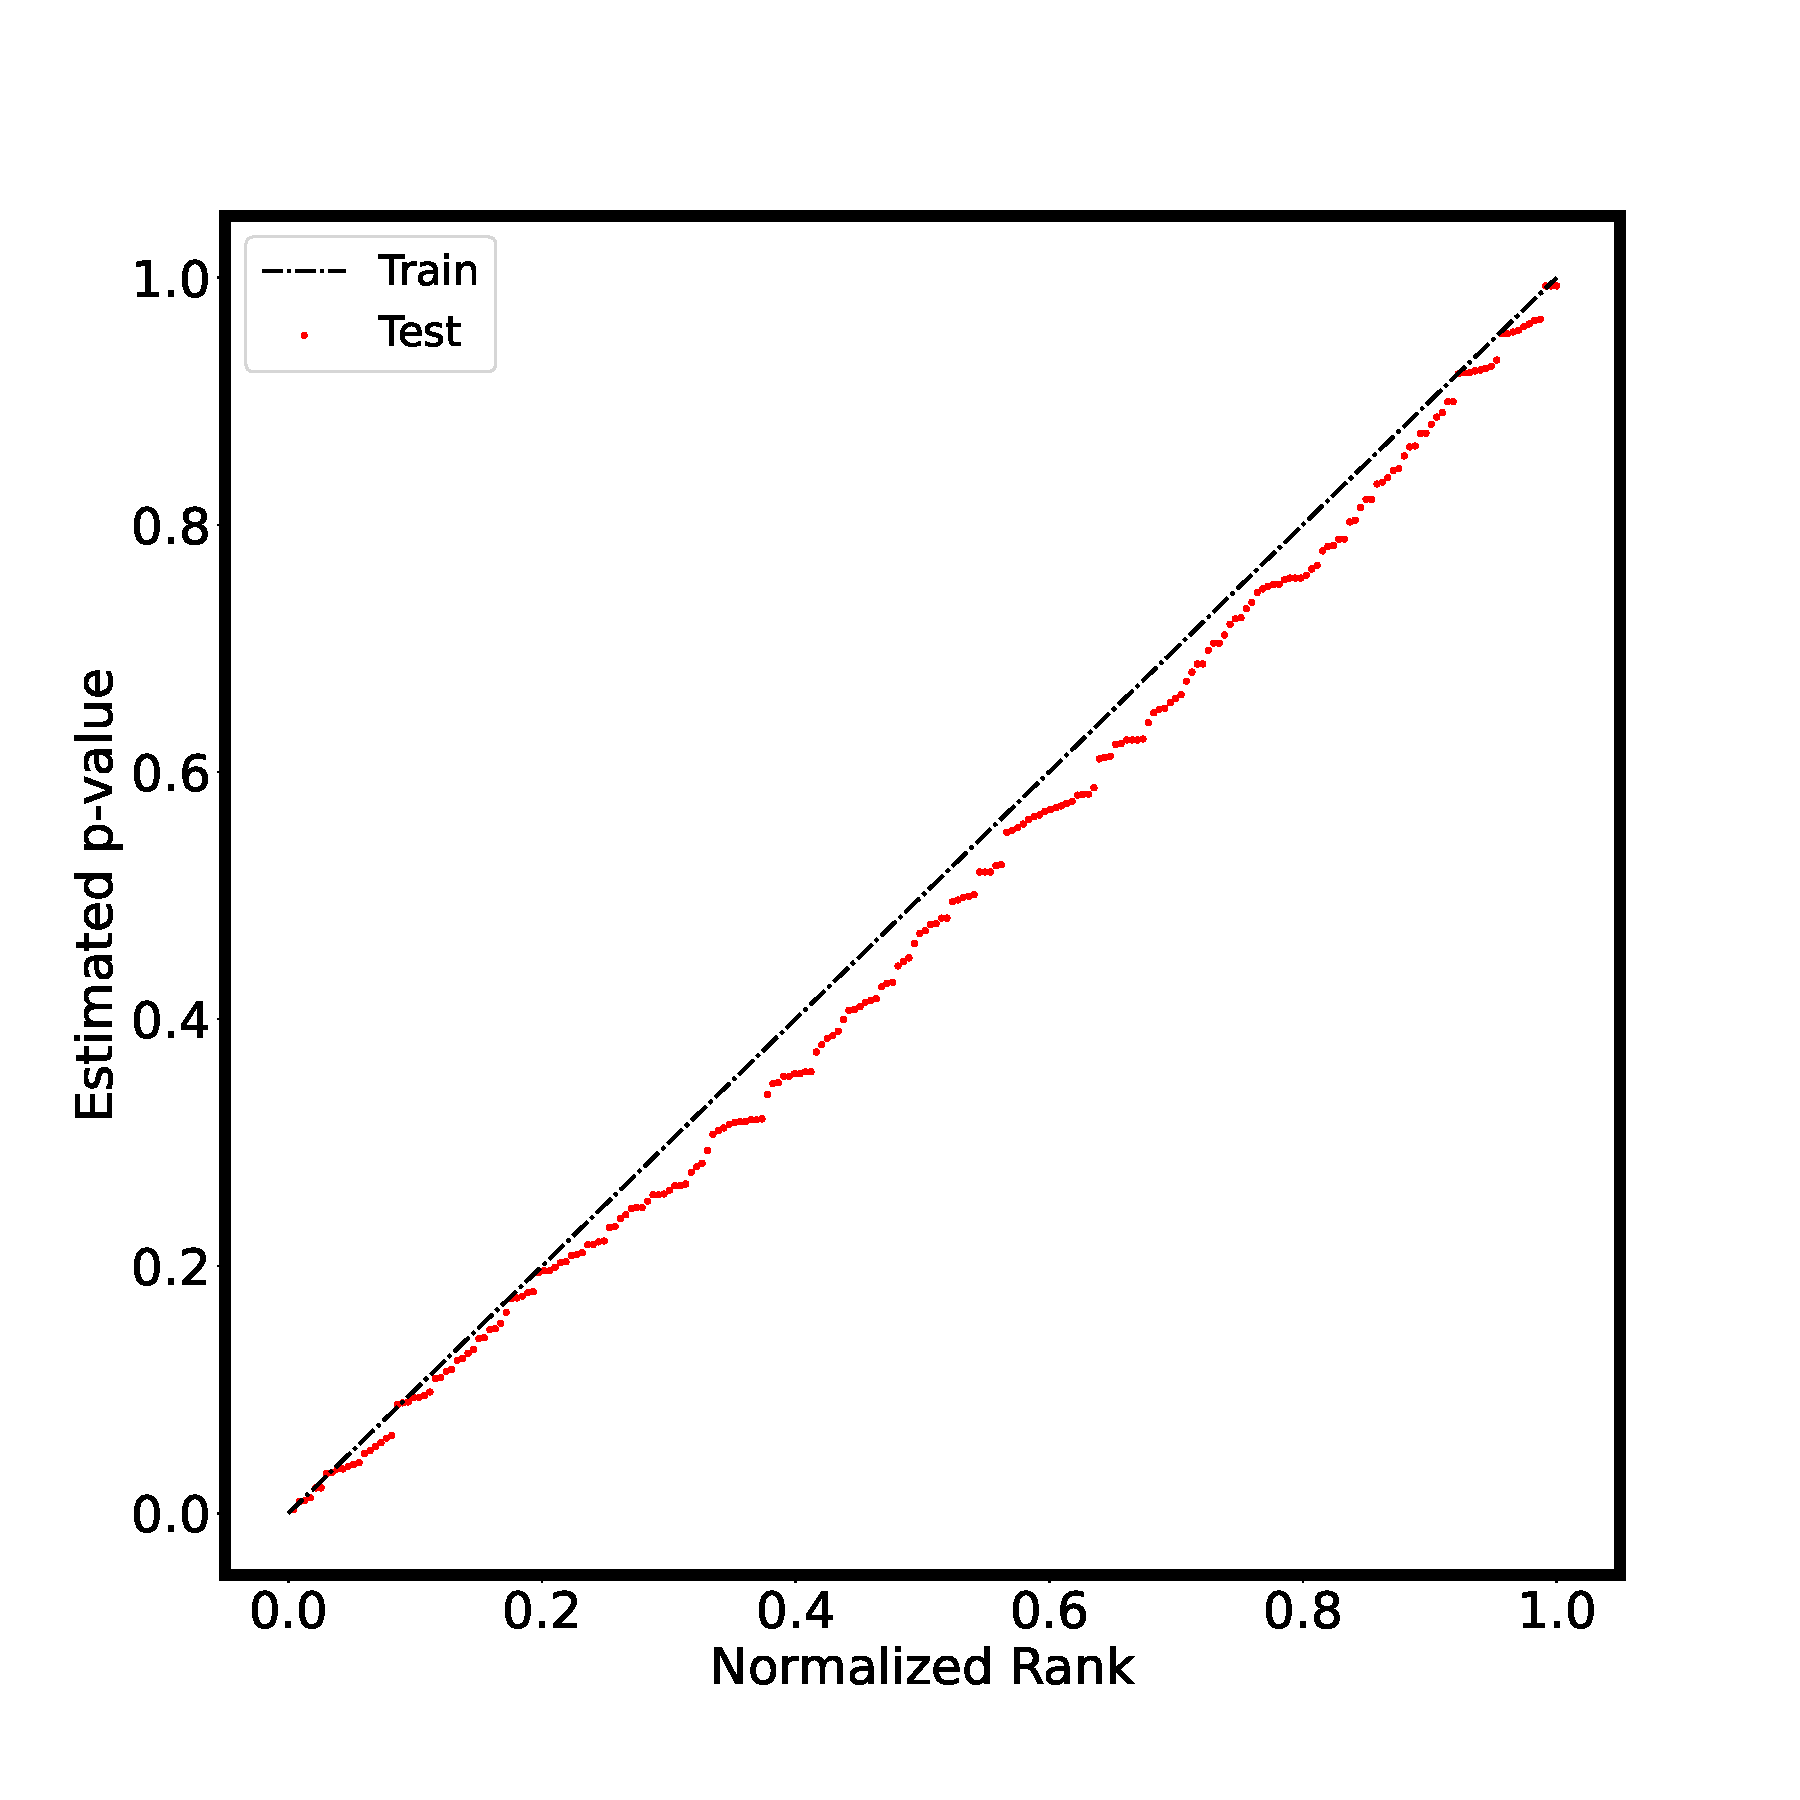
\includegraphics[width=3in]{img/cnn_QQ_multi.pdf} &
		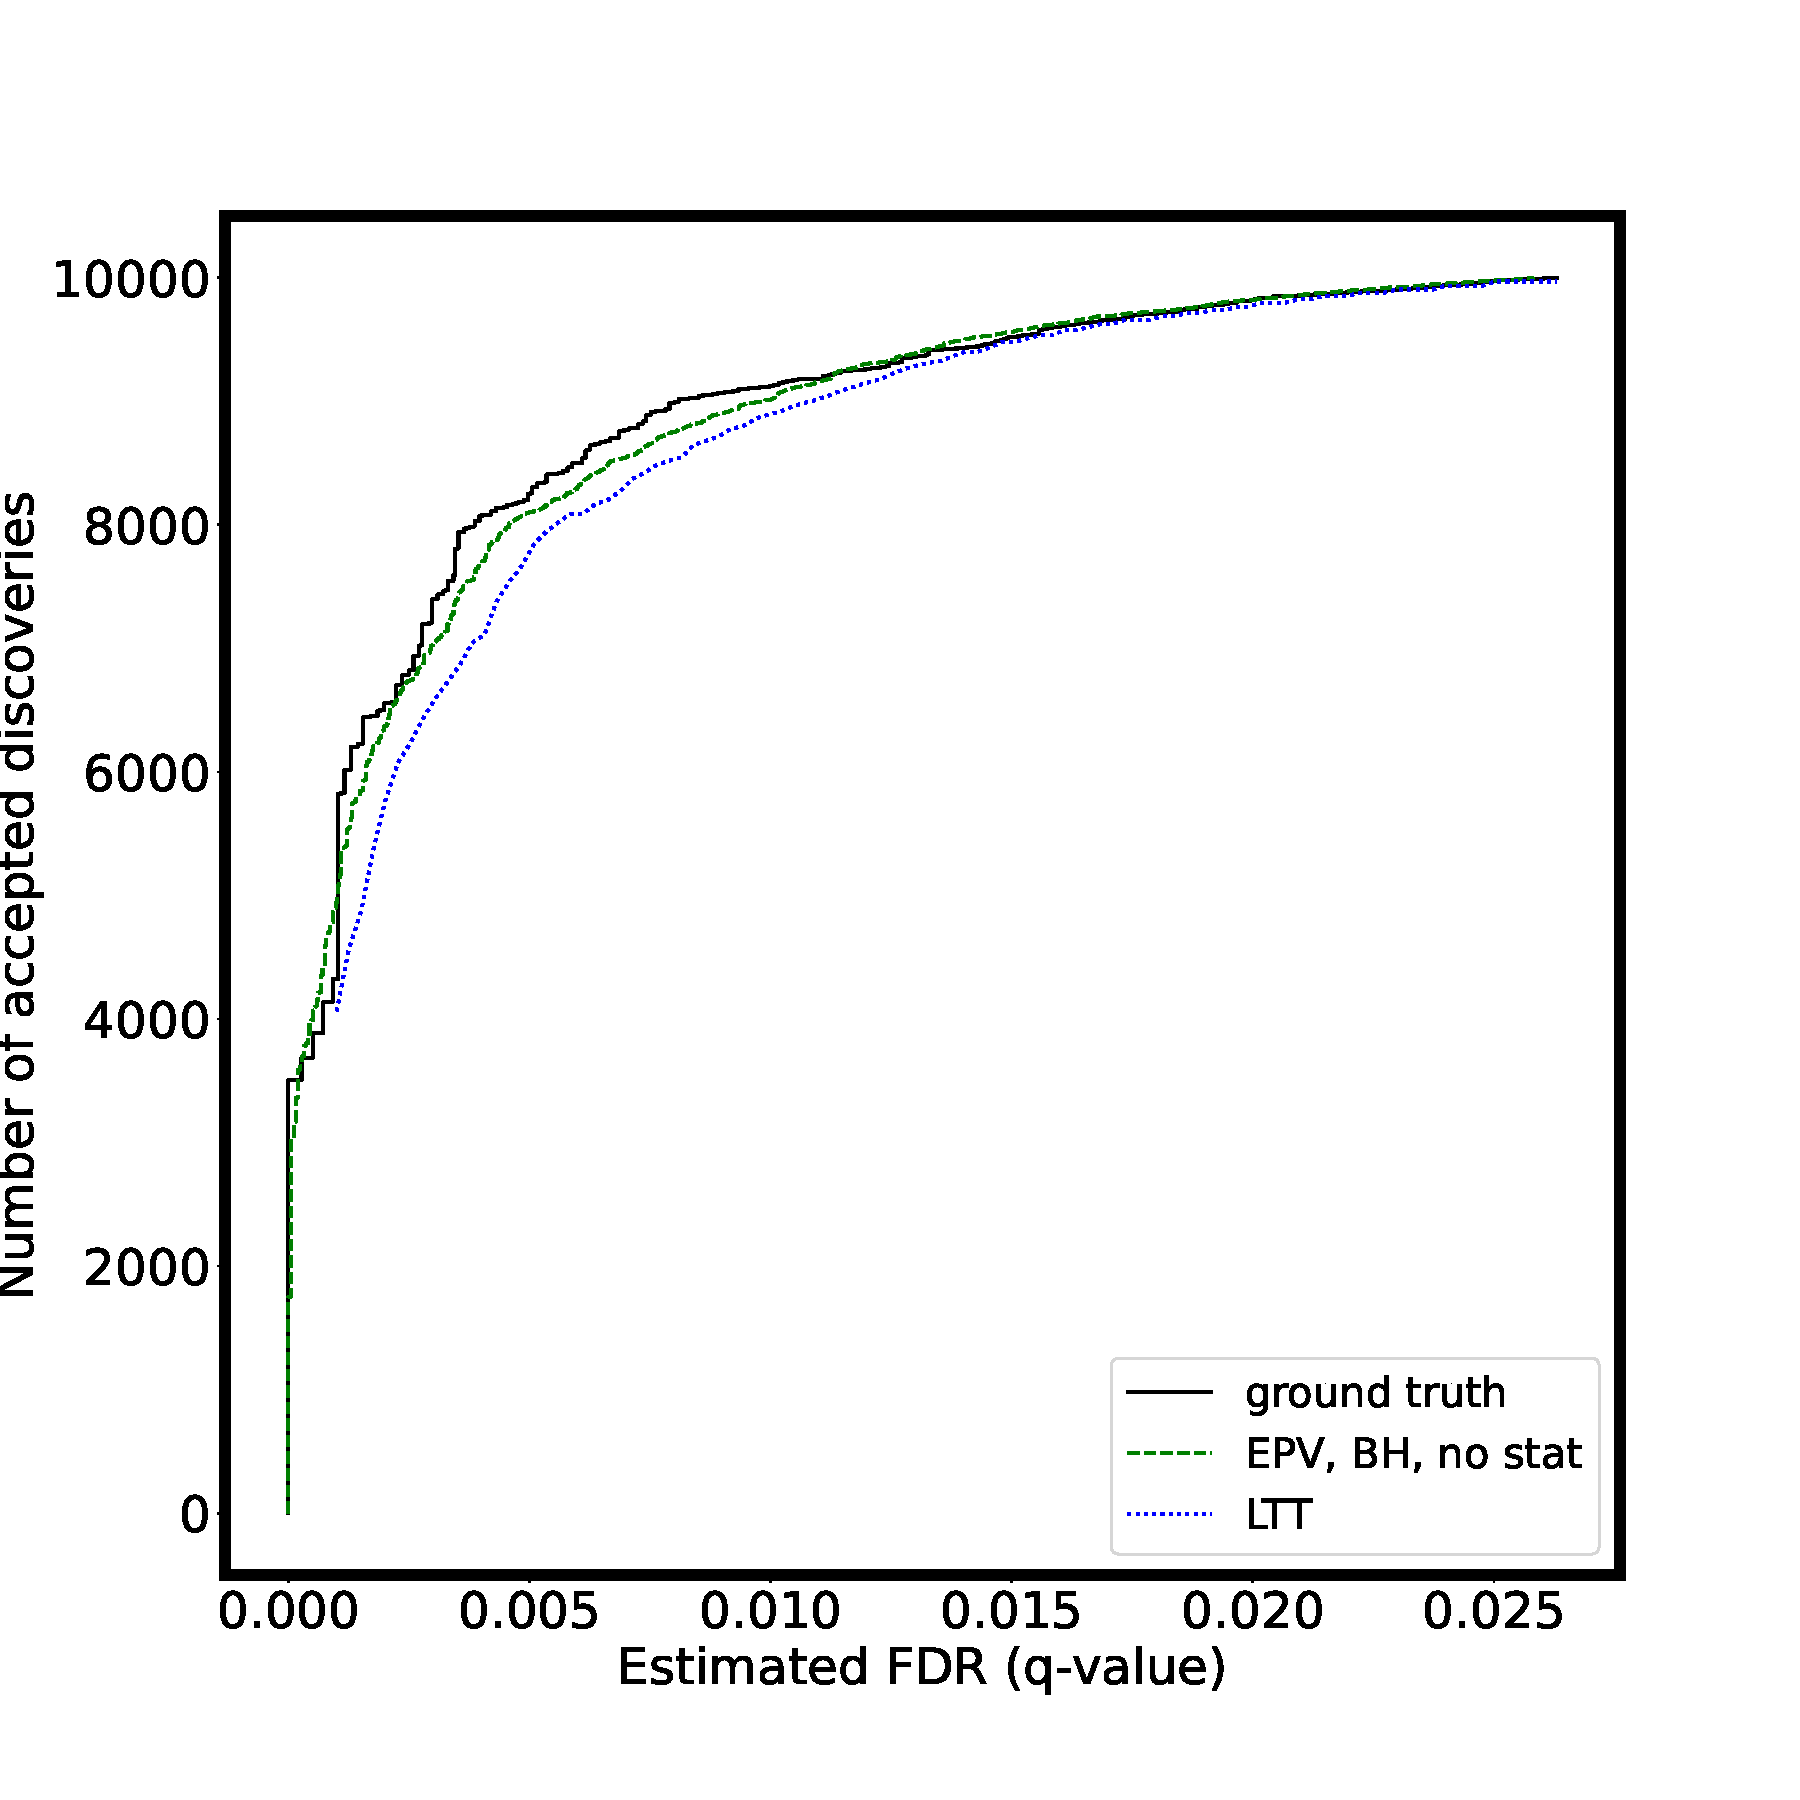
\includegraphics[width=3in]{img/cnn_multi_fdr_control.pdf} \\	
		A & B \\
	\end{tabular}
	\caption{{\bf FDR control with p-values for multi-class classification.}
		(A) a QQ plot of the p-values obtained with using negative training data. (B) The number of trusted classifications as a function of the FDR when it is controlled with true labels (red line) and with controlled with BHP (black line) using the p-values from panel (A).
		(A) a QQ plot of the p-values obtained with using training data classified as negative. (B) The same as panel (B), but using p-values from panel (C).
	}
	\label{fig:multi}
\end{figure}


\begin{figure}
    \advance\leftskip-0.5cm
        \begin{tabular}{ccc}
 		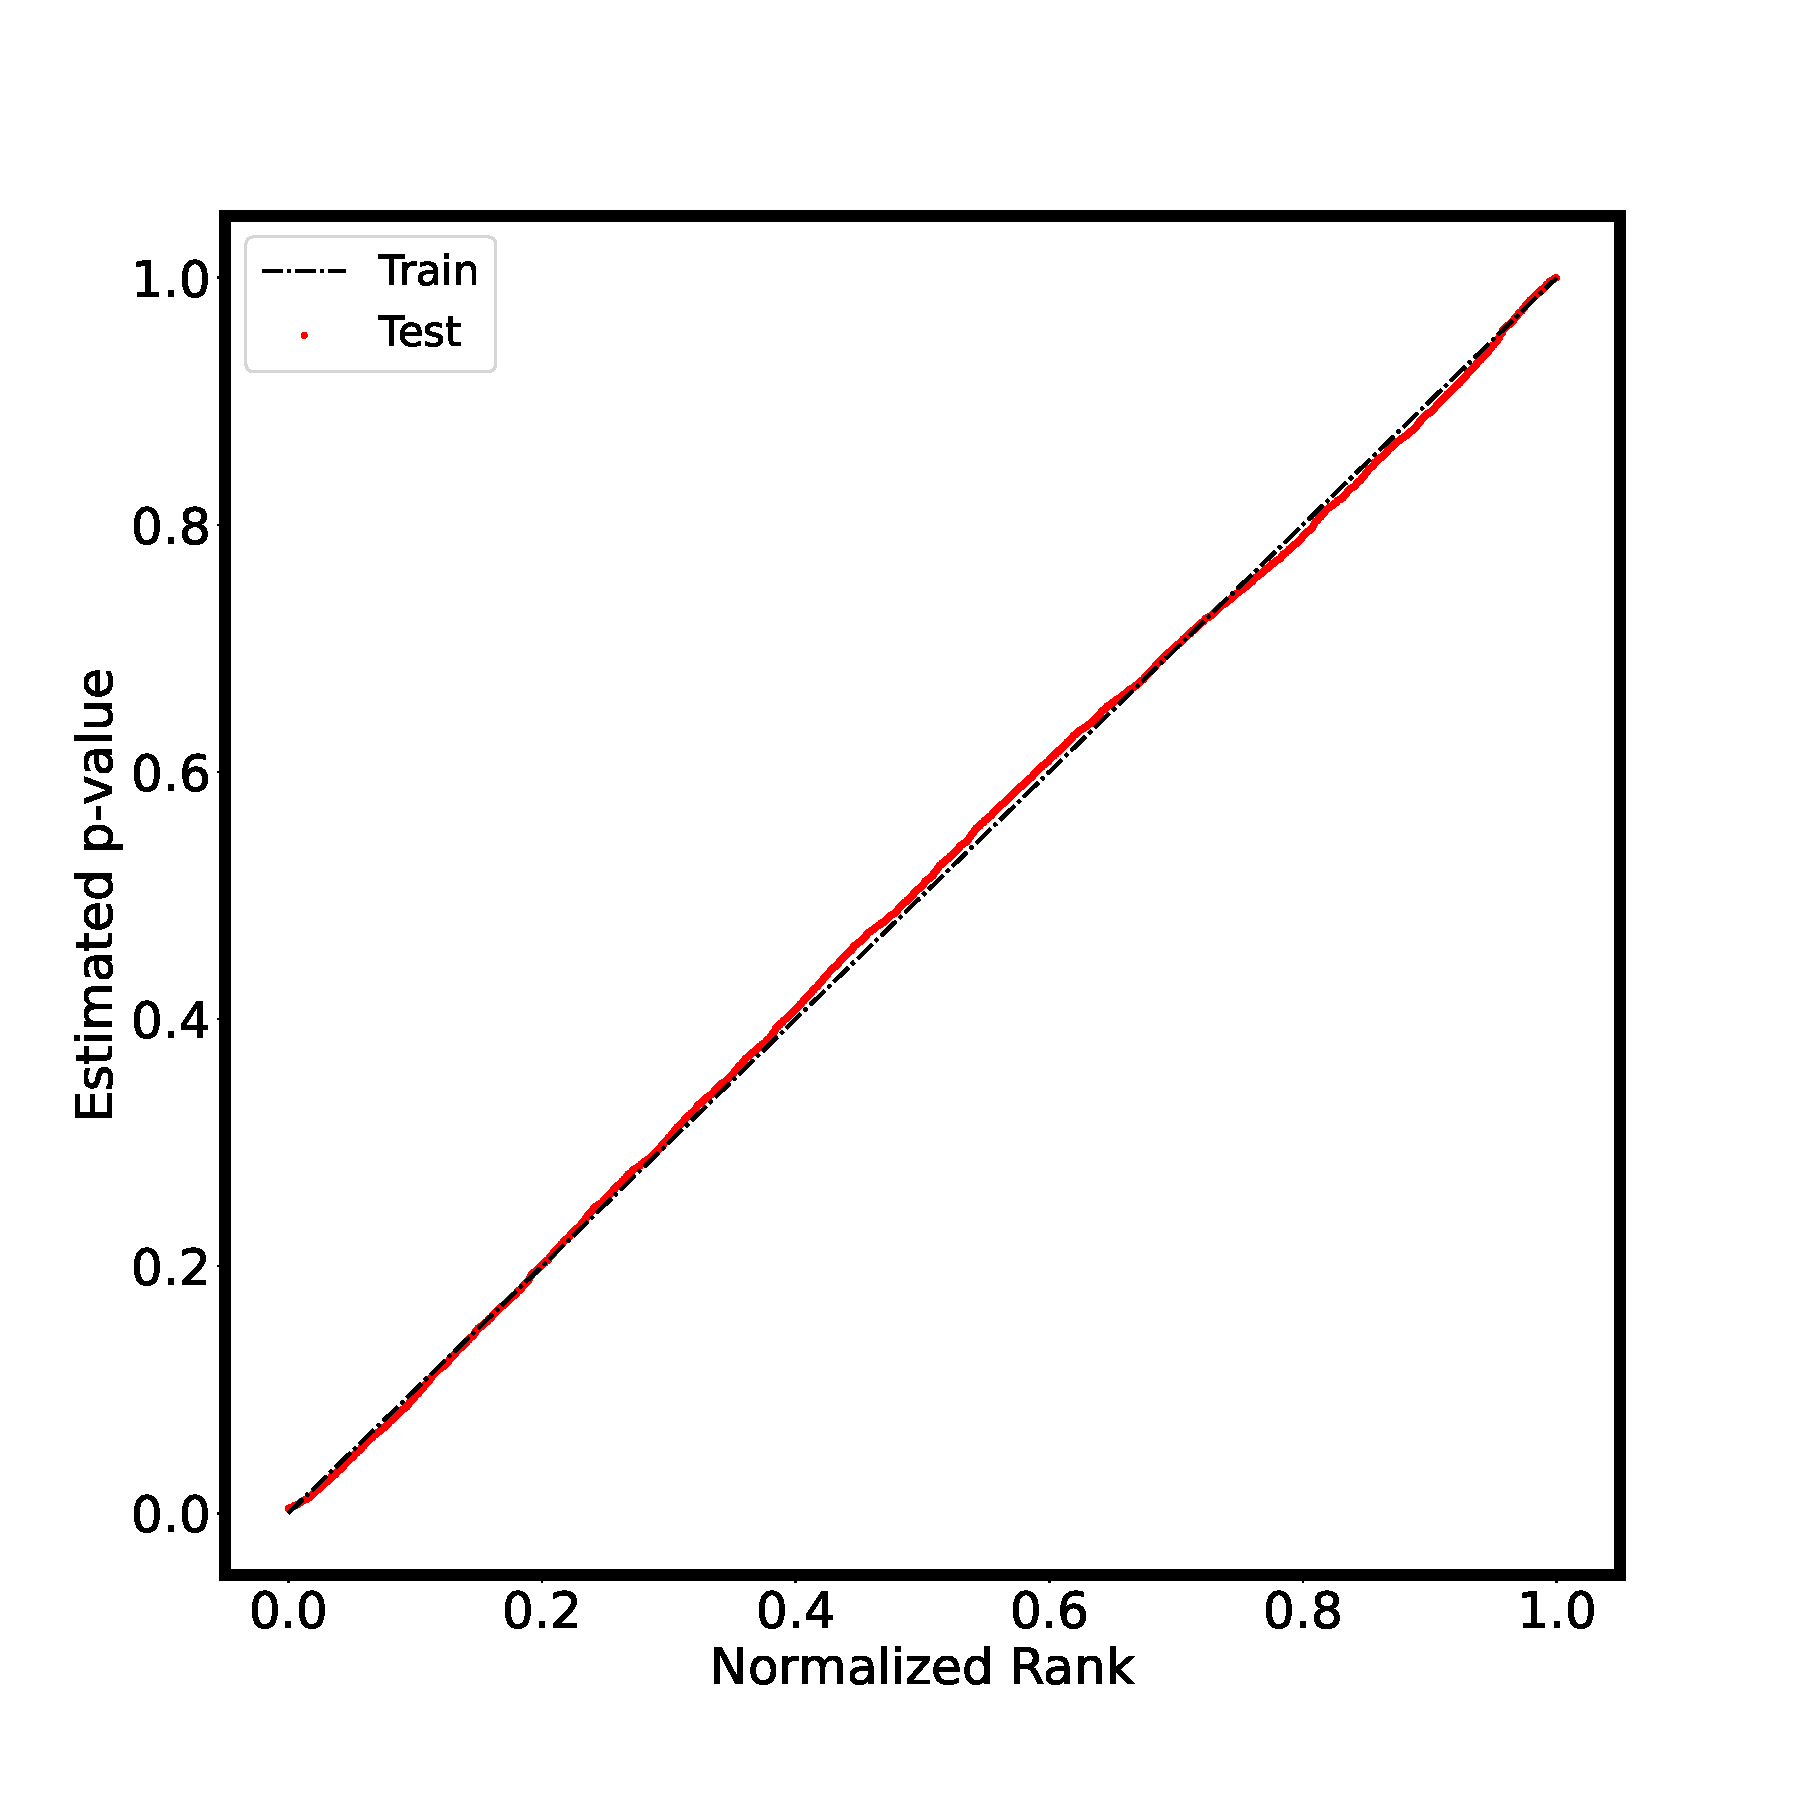
\includegraphics[width=2.5in]{img/cnn_QQ_shifted.pdf} &
		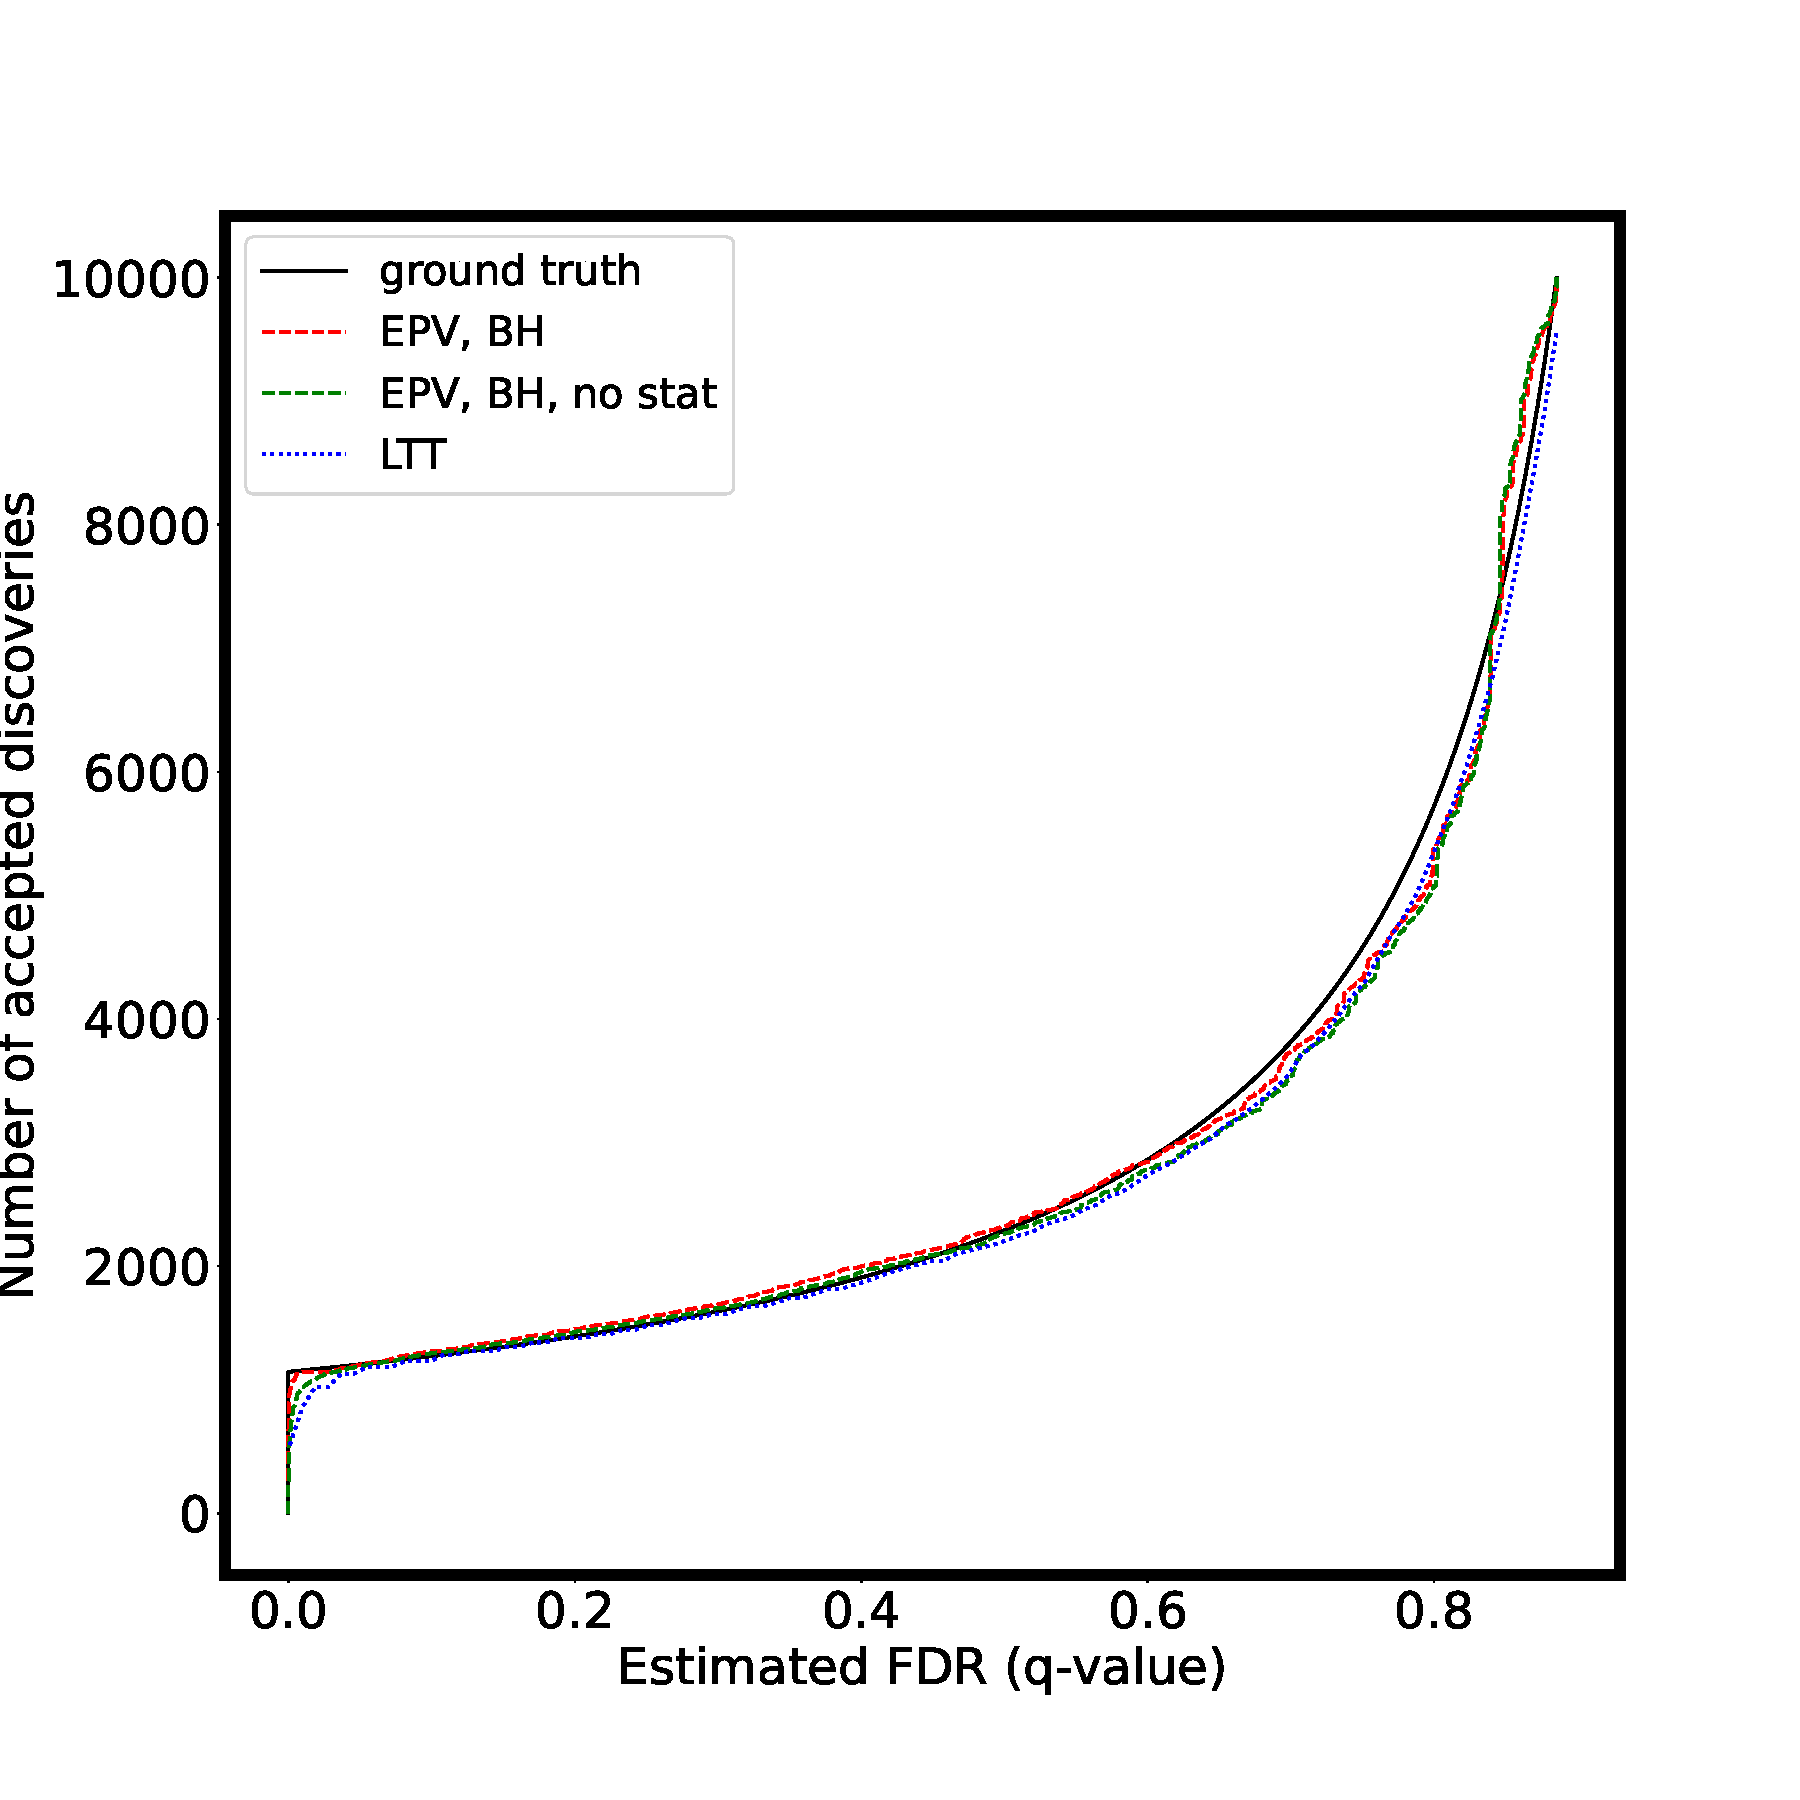
\includegraphics[width=2.5in]{img/cnn_shifted_fdr_control.pdf} & 
            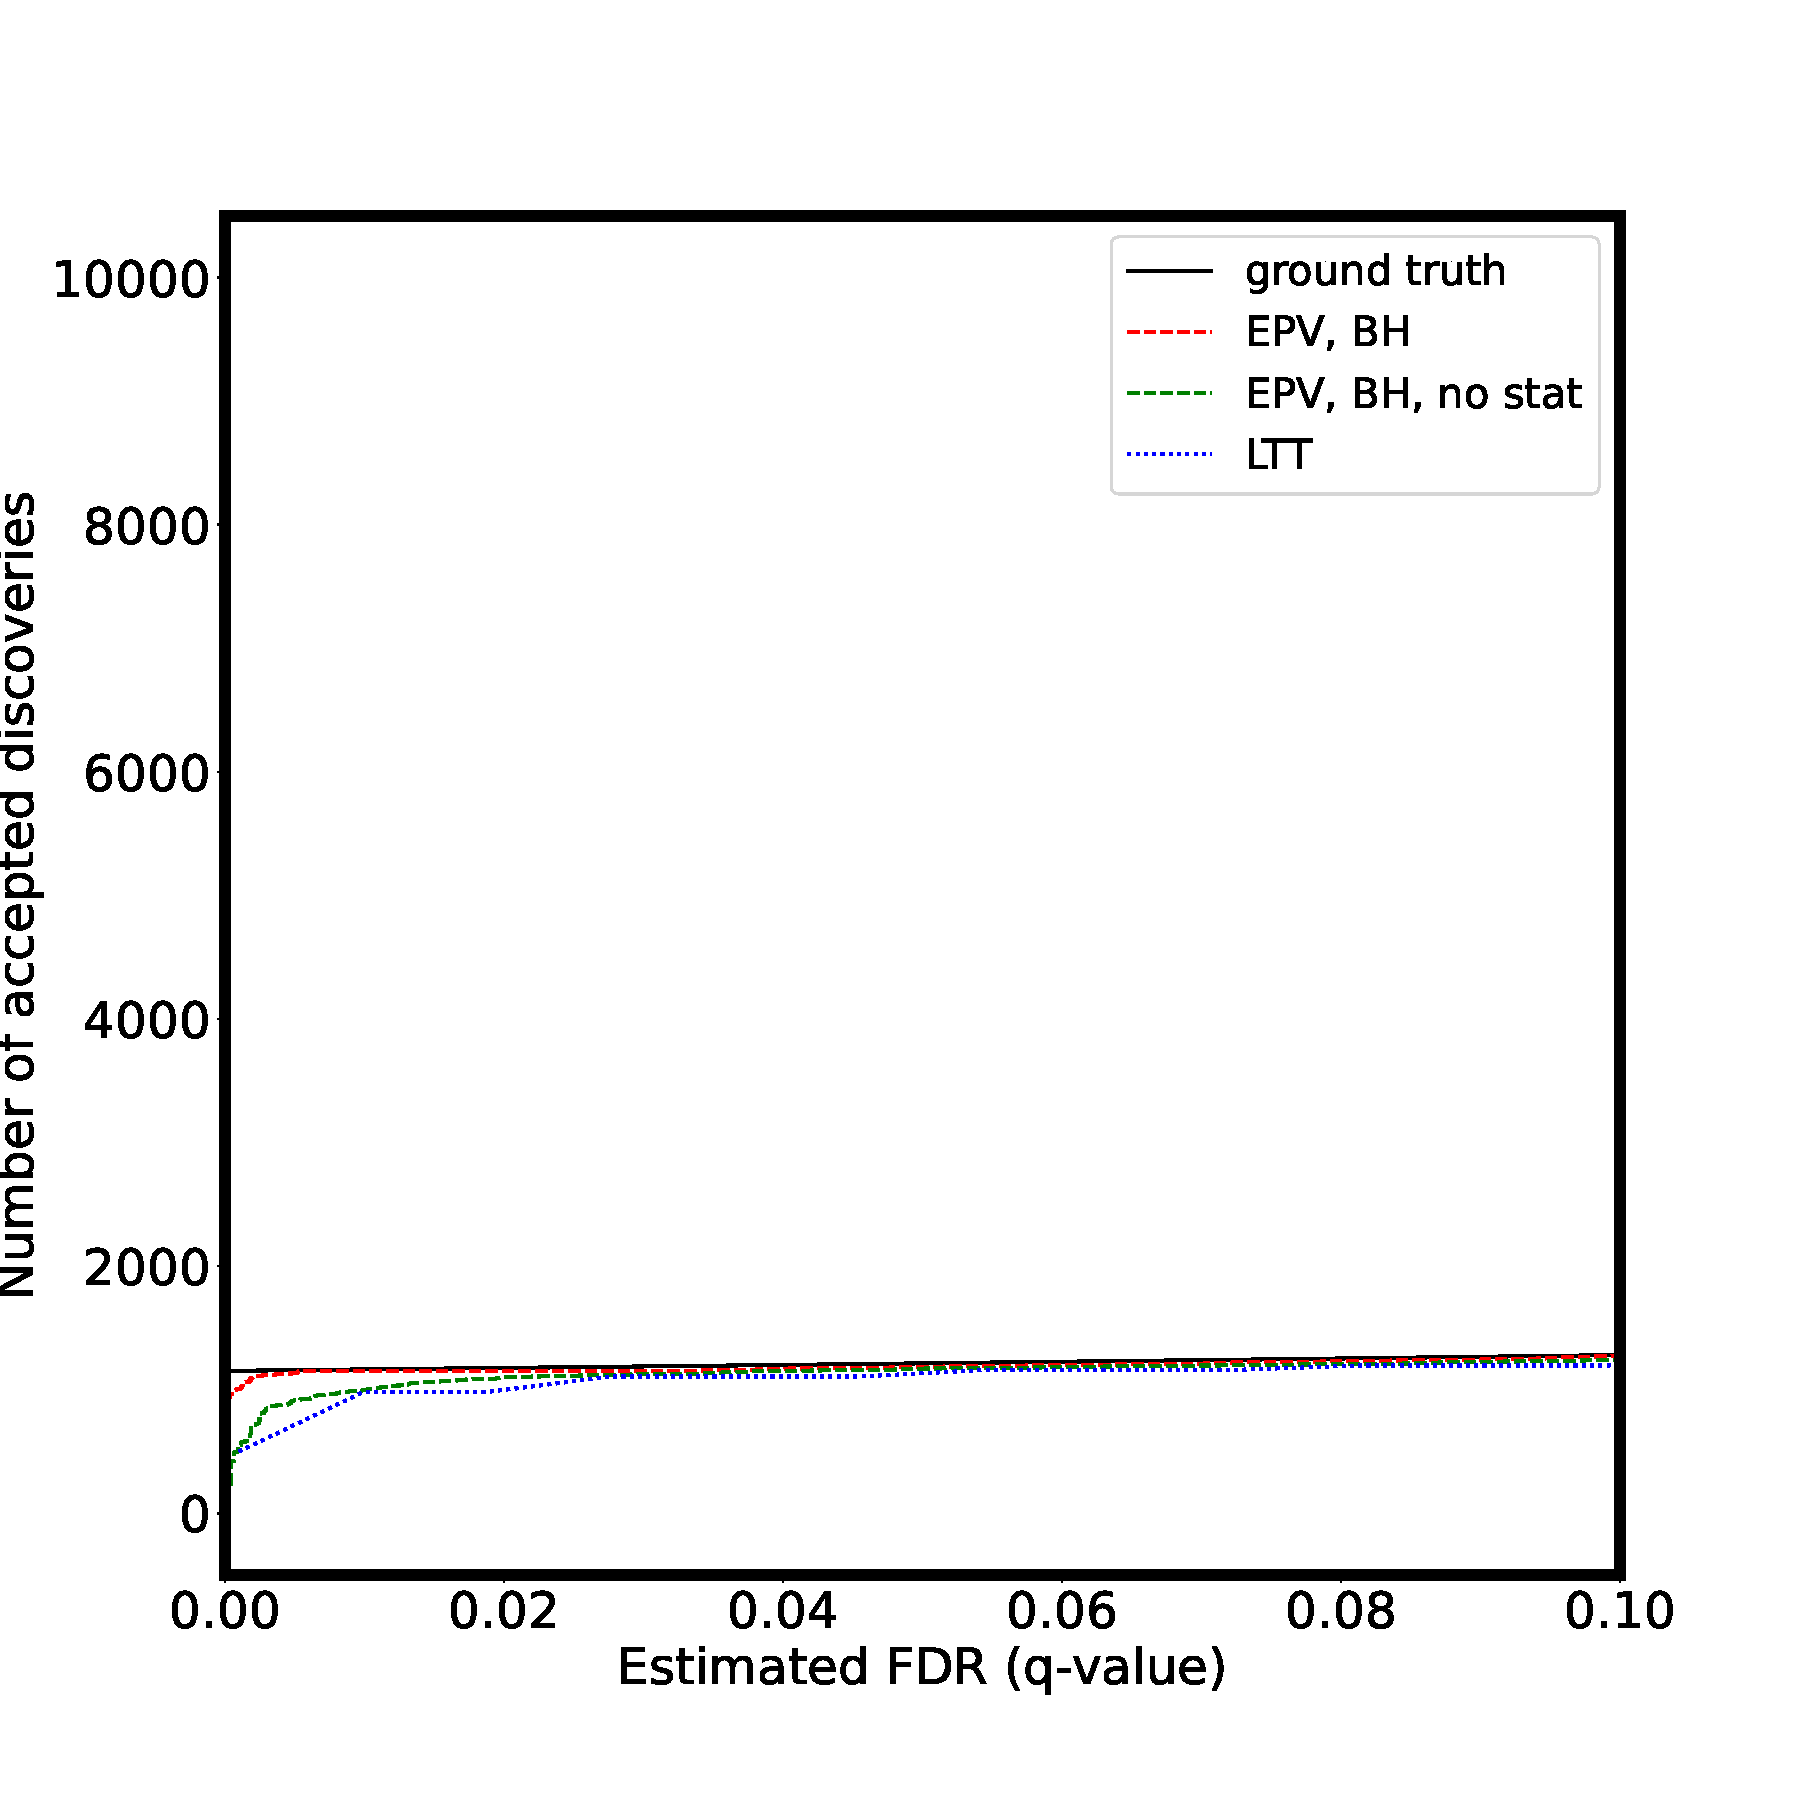
\includegraphics[width=2.5in]{img/cnn_shifted_fdr_control_loc.pdf}
		\\	
		A & B & C
	\end{tabular}
	\caption{{\bf  FDR control with p-values for detecting data distribution shift.}
		(A) a QQ plot of the p-values obtained with using negative training data. (B) The number of trusted classifications as a function of the FDR when it is controlled with true labels (red line) and with controlled with BHP (black line) using the p-values from panel (A).
		(A) a QQ plot of the p-values obtained with using training data classified as negative. (B) The same as panel (B), but using p-values from panel (C).
	}
	\label{fig:shift}
\end{figure}


\begin{figure}
    \advance\leftskip-0.5cm
        \begin{tabular}{ccc}
 		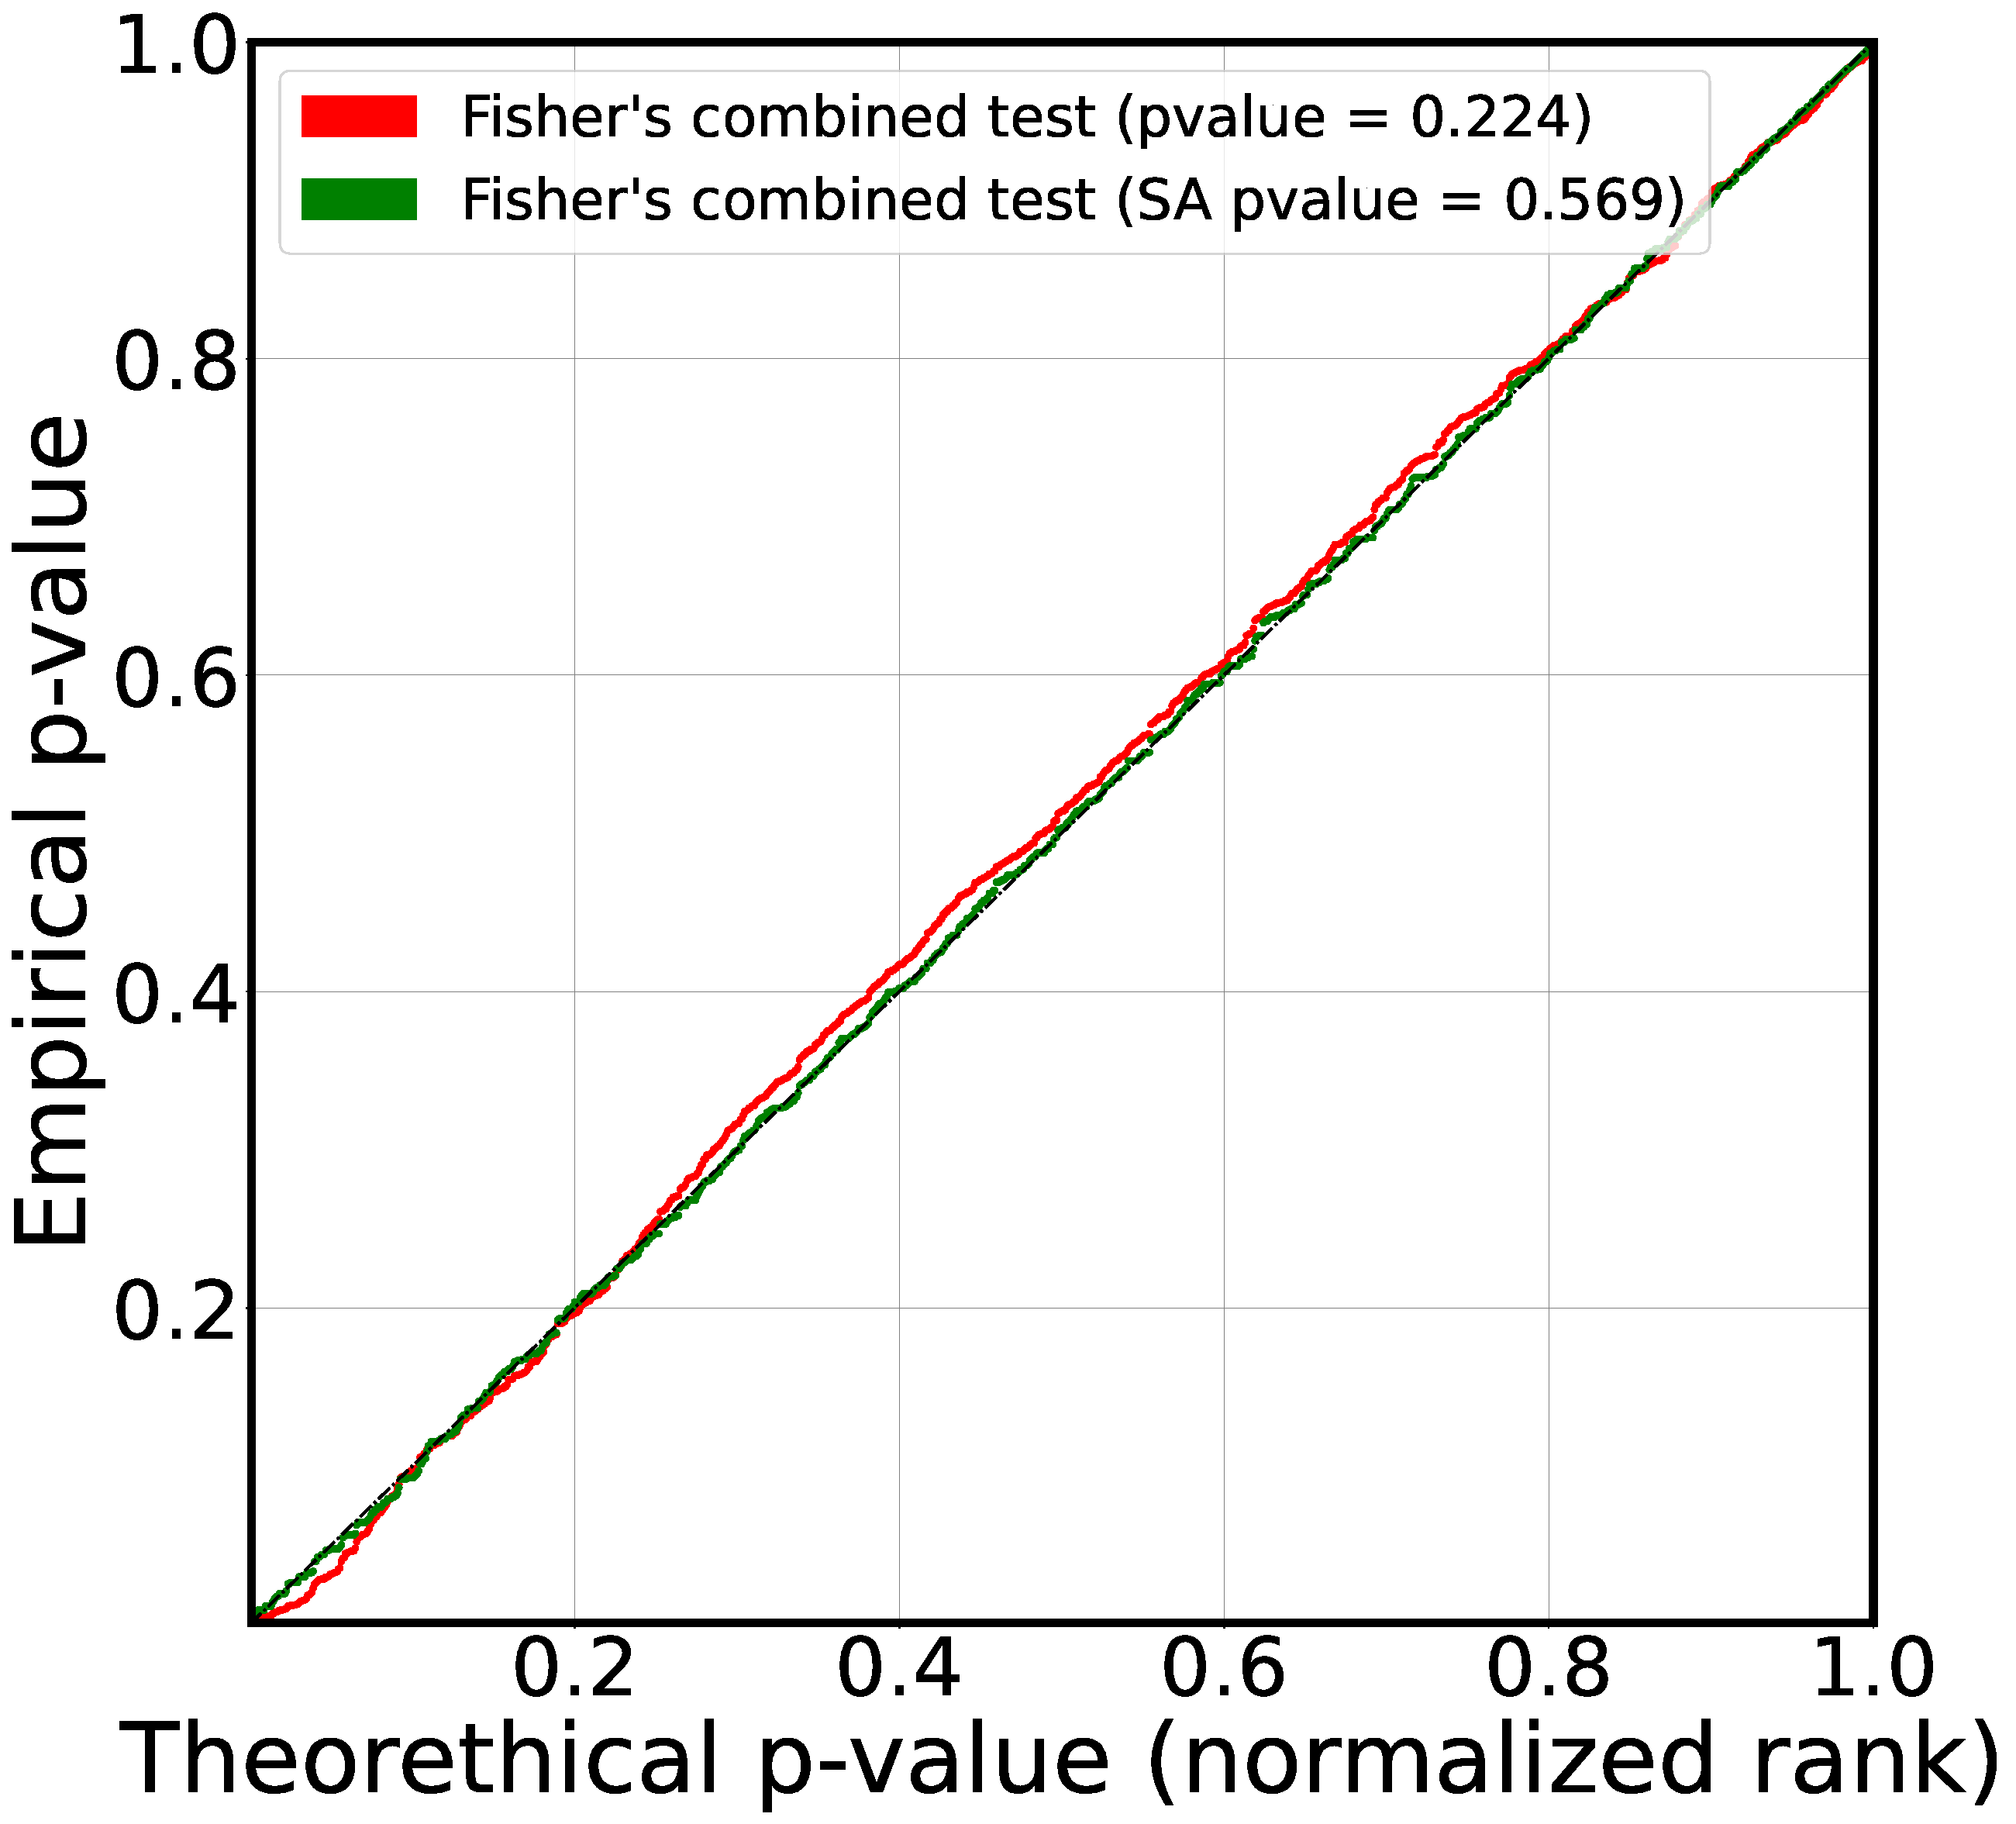
\includegraphics[width=2.5in]{img/cnn_QQ_balanced.pdf} &
		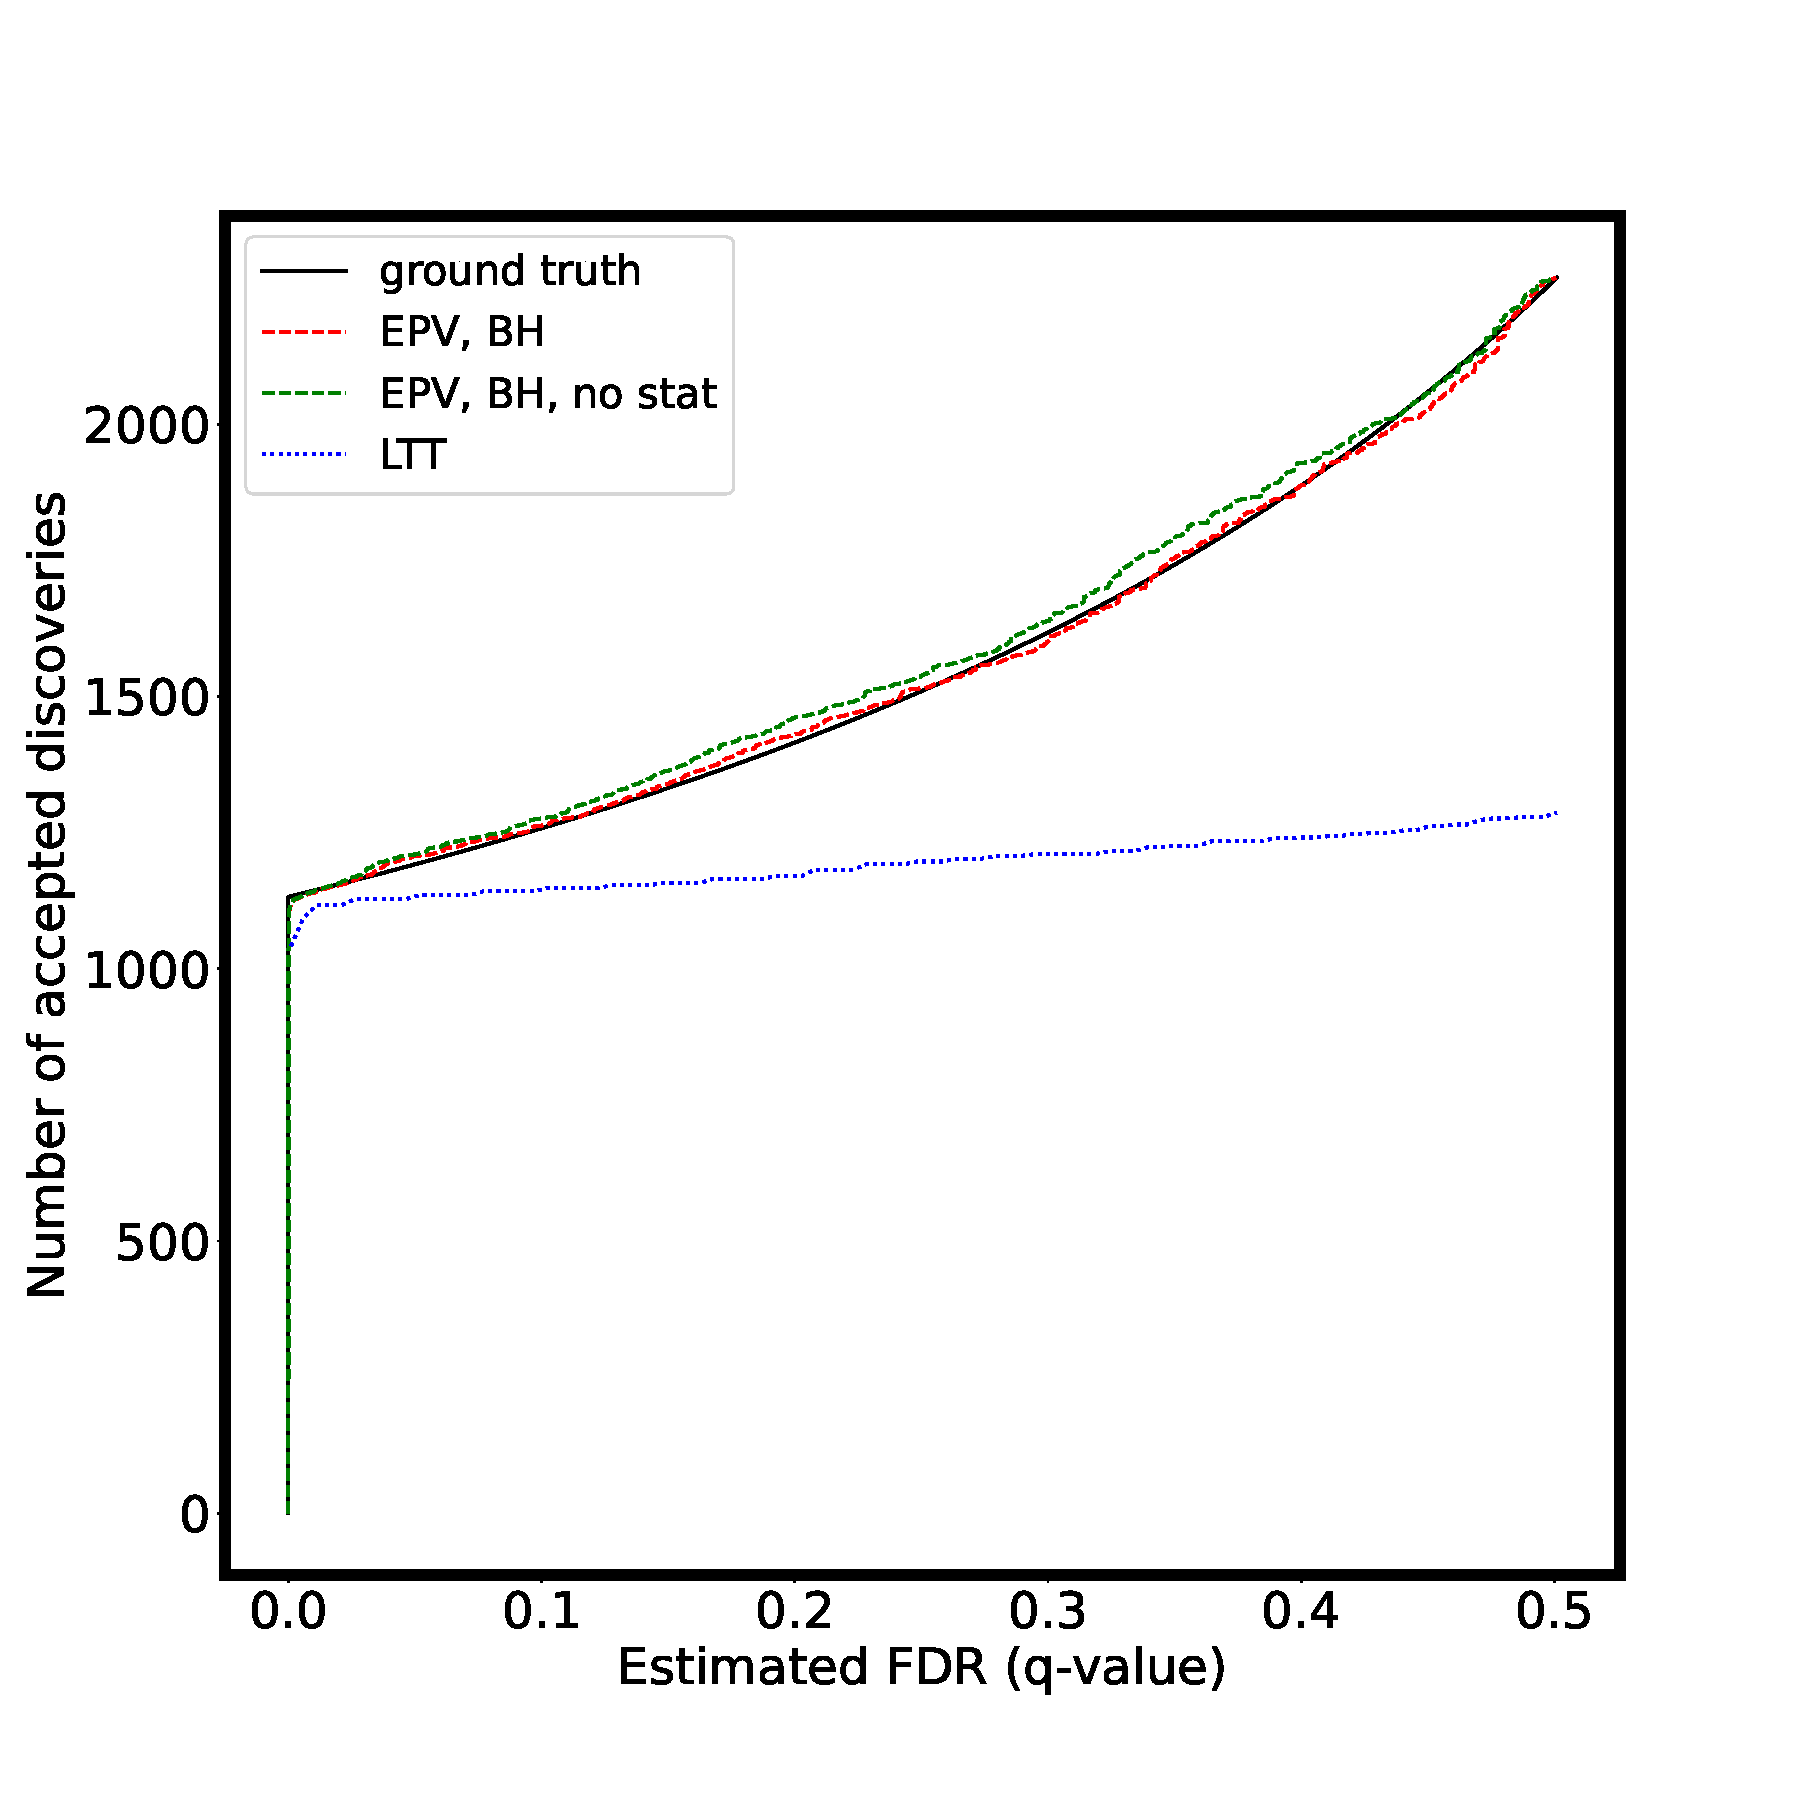
\includegraphics[width=2.5in]{img/cnn_balanced_fdr_control.pdf} & 
            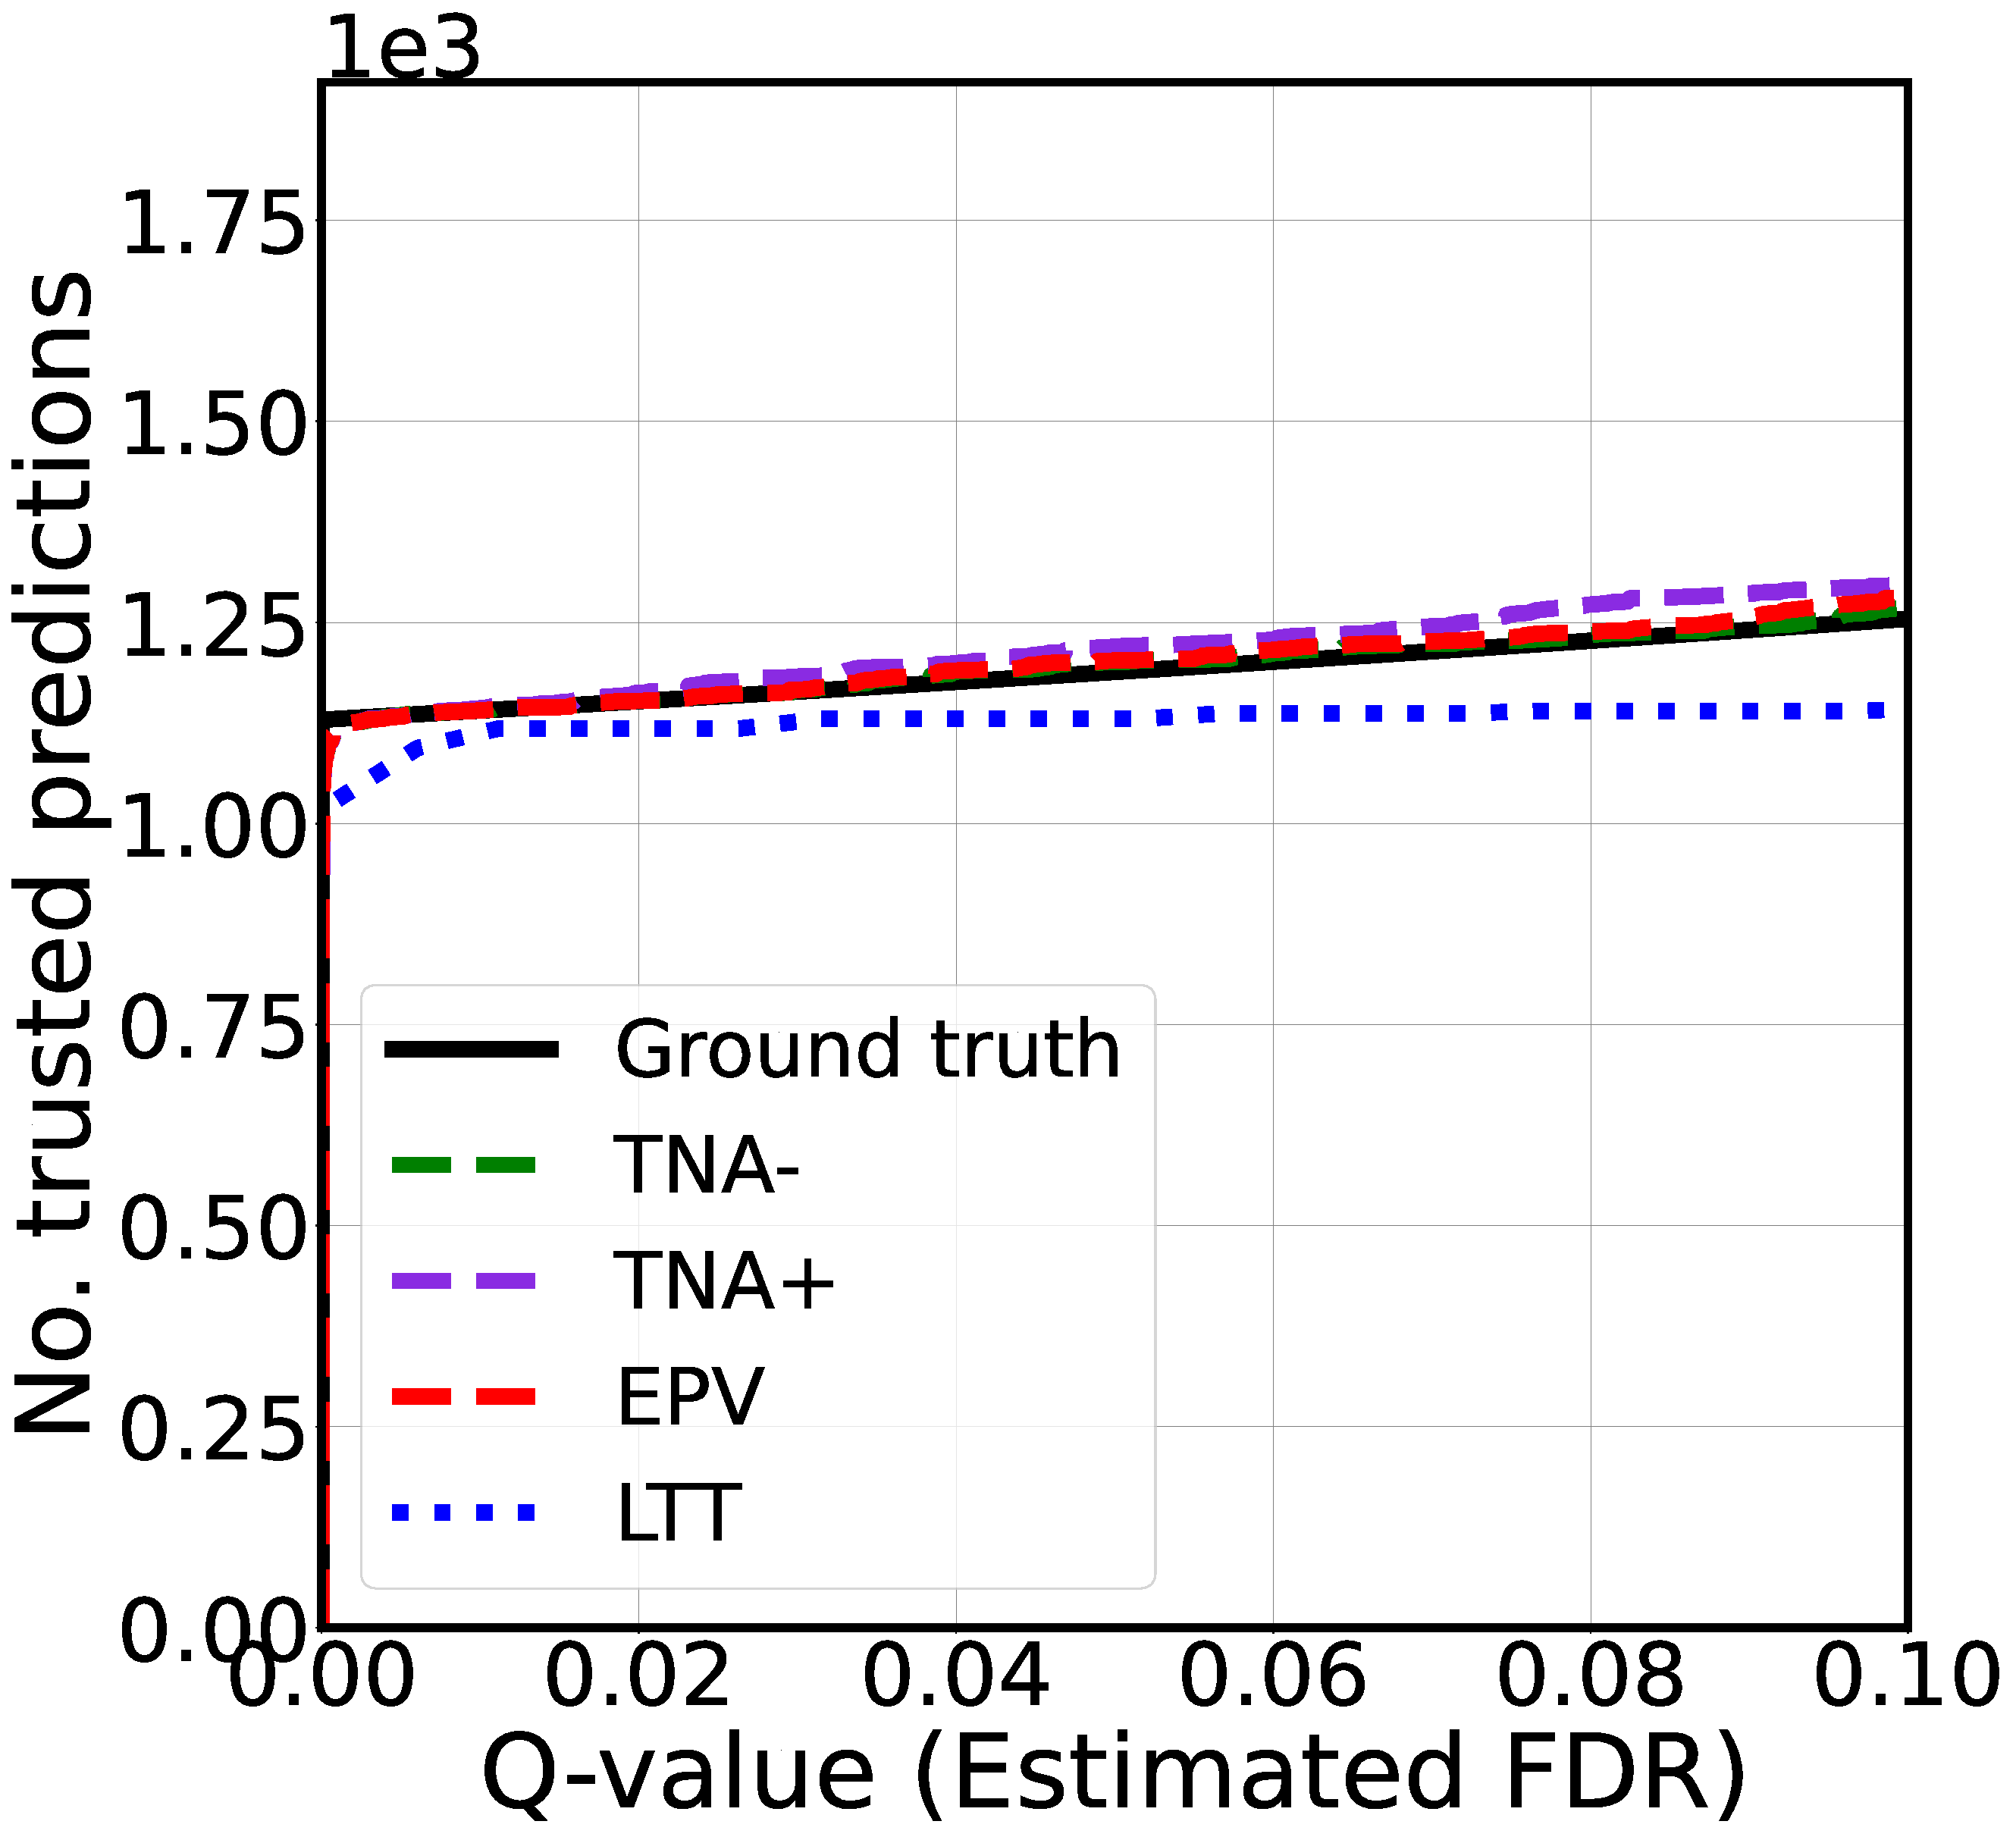
\includegraphics[width=2.5in]{img/cnn_balanced_fdr_control_loc.pdf}
		\\	
		A & B & C
	\end{tabular}
	\caption{{\bf  FDR control with p-values for altered class proportions.}
		(A) a QQ plot of the p-values obtained with using negative training data. (B) The number of trusted classifications as a function of the FDR when it is controlled with true labels (red line) and with controlled with BHP (black line) using the p-values from panel (A).
		(A) a QQ plot of the p-values obtained with using training data classified as negative. (B) The same as panel (B), but using p-values from panel (C).
	}
	\label{fig:balanced}
\end{figure}


\subsubsection{Multi-class case}

Another frequent problem statement is rather a number of classes with only one true label for each sample. The so-called multiclass classification implies getting simultaneously several scores as the model's output. At the same time, EPV approach necessitates separation of scores into negative and positive only. Thus, we insignificantly reformulate our workflow. Here, the p-value indicates significance a sample being correctly classified. Then, we work only with the greatest scores among all presented, and the null distribution is constructed from the maximum values for the entire miss-classified training data. Thereby, we aim to control that whether a test data is correctly classified to its class or not. The $\pi_0$, again is estimated by the proportion of the incorrect classification among all samples. It is a tiny number due to chosen high-performance model in context of resolvable MNIST dataset.

Getting closer to the graphs, we should outline that only two plots were acquired. Such a situation is still a consequence of CNN superior results, when the error does not exceed several percents. Hence, we could only work with FDR on a very little range. Nevertheless, a little fall of quality compared to binary case can be seen on QQ plots. At the same time, EPV still appears to be adjacent to the diagonal at each point with a reasonable maximum distance. If moving to the FDR graph, one can see that EPV together with BH protocol still outperform LTT, preserving a high level of interpretability as a smoother version of ground truth. 

\subsubsection{Shift case}

As it was declared, MNIST has a set of properties, making it improper for a comprehensive analysis. For instance, it does not allow to check whethever methods are resilient to shifts in data distribution. Therefore, we trained the CNN on described binary task with preserved target label "2". However, for further examination of p-values’ nature, we introduce a 1-by-1 pixel move for each image. The newly born samples with shifted data distribution depict such a scenario, when upcoming test data has a visible difference from training phase. 

So, the final part of the experiment implies running the altered images through the already trained model. On the resulting graphs, we can identify the first perceptible limitation of our EPV methodology. While it keeps maintaining a notable proximity to the ground truth plot in terms of the first 10\%, the rest of the range depict a significant rightward shift. At the same time, LTT, also experiencing difficulties, shows much better results on a long-run. Another evidence of EPV's inconsistency in case of data shifts is depicted on the QQ plot, where the test dots make a sufficient drift from the diagonal. 

The reason for such a behavior is that for our particular experiment's environment a shift can be identified not only in data distribution, but also in scores distribution. The left boundary of test results has made a serious leftwards shift, meaning far more test cases started obtaining a unit p-value (1.0). This is why the EPV algorithm has such a drastic growth, when reaching the maximum FDR level.

In order to deal with this, we propose to implement such an activation function to the given set of scores that will encapsulate all the values in a specific range during inference mode only. For instance, sigmoid can be used. Such a strategy allows to make our algorithm more resistant to any significant alterations in data distribution, whcih can be seen on the correspoding graph.


However, the emerged QQ plots have shown a radical alteration compared to the preceding graphs. The comparison outlines the p-values’ initial uniform distribution’s elimination. 

\subsubsection{Balance case}

Final conditions to be described imply another form of dataset's alteration. However, this time the proportion of positive and negative classes is changed rather than the data itself. Instead of inferring on the entire available test dataset, we collect all the positive samples (composing only 10 percent) and append the equal amount of negative samples in accordance with true labels for the sake of experiment's requirements. The declared parity differs from the share of classes, which the model has seen during training. Hence, a highly probable real-life scenario is tested here.

Again, straightforward implementation of EPV without any statistical corrections was leading to the low algorithm's ability to describe the ground truth. However, transferring the entire approach into the current form made a drastic amelioration. As it can be seen on figure \ref{fig:balanced}, our method plus BH protocol work almost perfectly, with a little bit higher number of discoveries predicted on the local range. On the contrary, the LTT framework, based on FWER-family approach, shows comparatively dreary results, behaving illogically in terms of ground truth. If moving to the \ref{fig:balanced}A, we can see ultimately close scatter plot to the "Train" diagonal.

\subsection{Biomedical data: tumor classification}

\begin{figure}
	\centering
	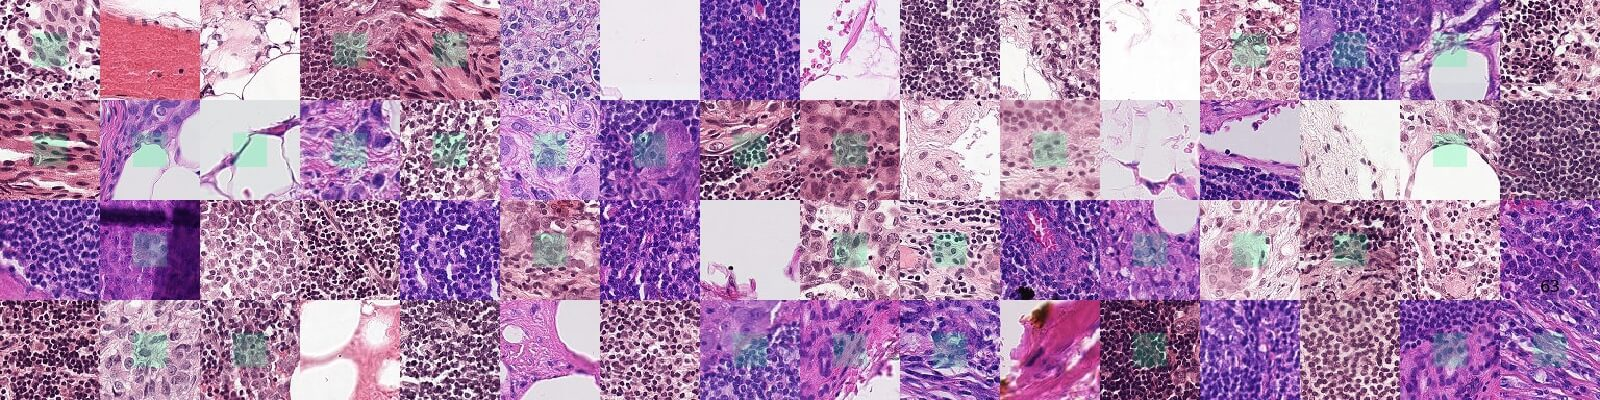
\includegraphics[width=6in]{img/pcam_example.png}
	\caption{{\bf Instances of PCam dataset.} Green boxes indicate tumor tissue in center region, which dictates a positive label.}
	\label{fig:pcam_example}
\end{figure} 

Medical imaging itself becomes an area of elevated attention during last years of machine learning development. Various areas are found on the intersection of medicine and bioinformatics annually. Moreover, identification of disease presence by AI, while being an exhaustive topic of interest, cultivates the need in strict control over the chance of FP error. Thereby, we present a set of various biomedical datasets for classification task, each being analyzed by the proposed algorithm.

\subsubsection{Datasets and Models}

The PatchCamelyon (PCam) benchmark dataset is a fairly rich collection of histopathologic scans of lymph node sections. It consists of 327.680 colored images of size (96, 96) each. The provided task demands performing a binary classification, identifying the presence or absence of any histopathology. PCam was deduced from Camelyon16 dataset by splitting images into patches. However, it appears to be far easier in generalization by the neural networks, in turn still showing a high accuracy in metastasis detection on the ancestor. We believe this is a relevant clinical task, which strives to have the control over the possible error rate.

The creators underscore that all the subsets - training, validation, test - are equally divided, persisting the class balance of 1:1. Moreover, the patches do comprise a synthetic beginning since the tumor cells could be found only in the centre region of the image with size (32, 32). Nevertheless, authors still provide the outer region for model's compliance with Camelyon16, but they do slightly lighten the task by reducing the area of interest.

For the sake of proving practicality of our method, we will manually change the classes' proportions. However, no data distribution shift could be performed except the one laid in test subset.

Speaking of the model, we rely on the pretrained neural network from the \href{https://tiatoolbox.readthedocs.io}{TIA toolbox}. This toolbox for tissue image analysis provides a torch-written API with distinct efficient algorithms for a bunch of various biomedical tasks. Except the trained models themselves, package also introduces tools for data loading, pre- and post-processing, visualization together with the overall inference. For the PCam dataset, TIA package suggest over a dozen of models. We chose the \href{https://huggingface.co/1aurent/resnet34.tiatoolbox-pcam}{resnet34-pcam}. It is the ubiquitously known model from the torchvision deep residual learning collection being further advanced by TIA research centre with the use of PCam data.

\todo{andrey}{accuracy of model}

\subsubsection{Standard case}

\begin{figure}
	\advance\leftskip-0.5cm
	\begin{tabular}{ccc}
 		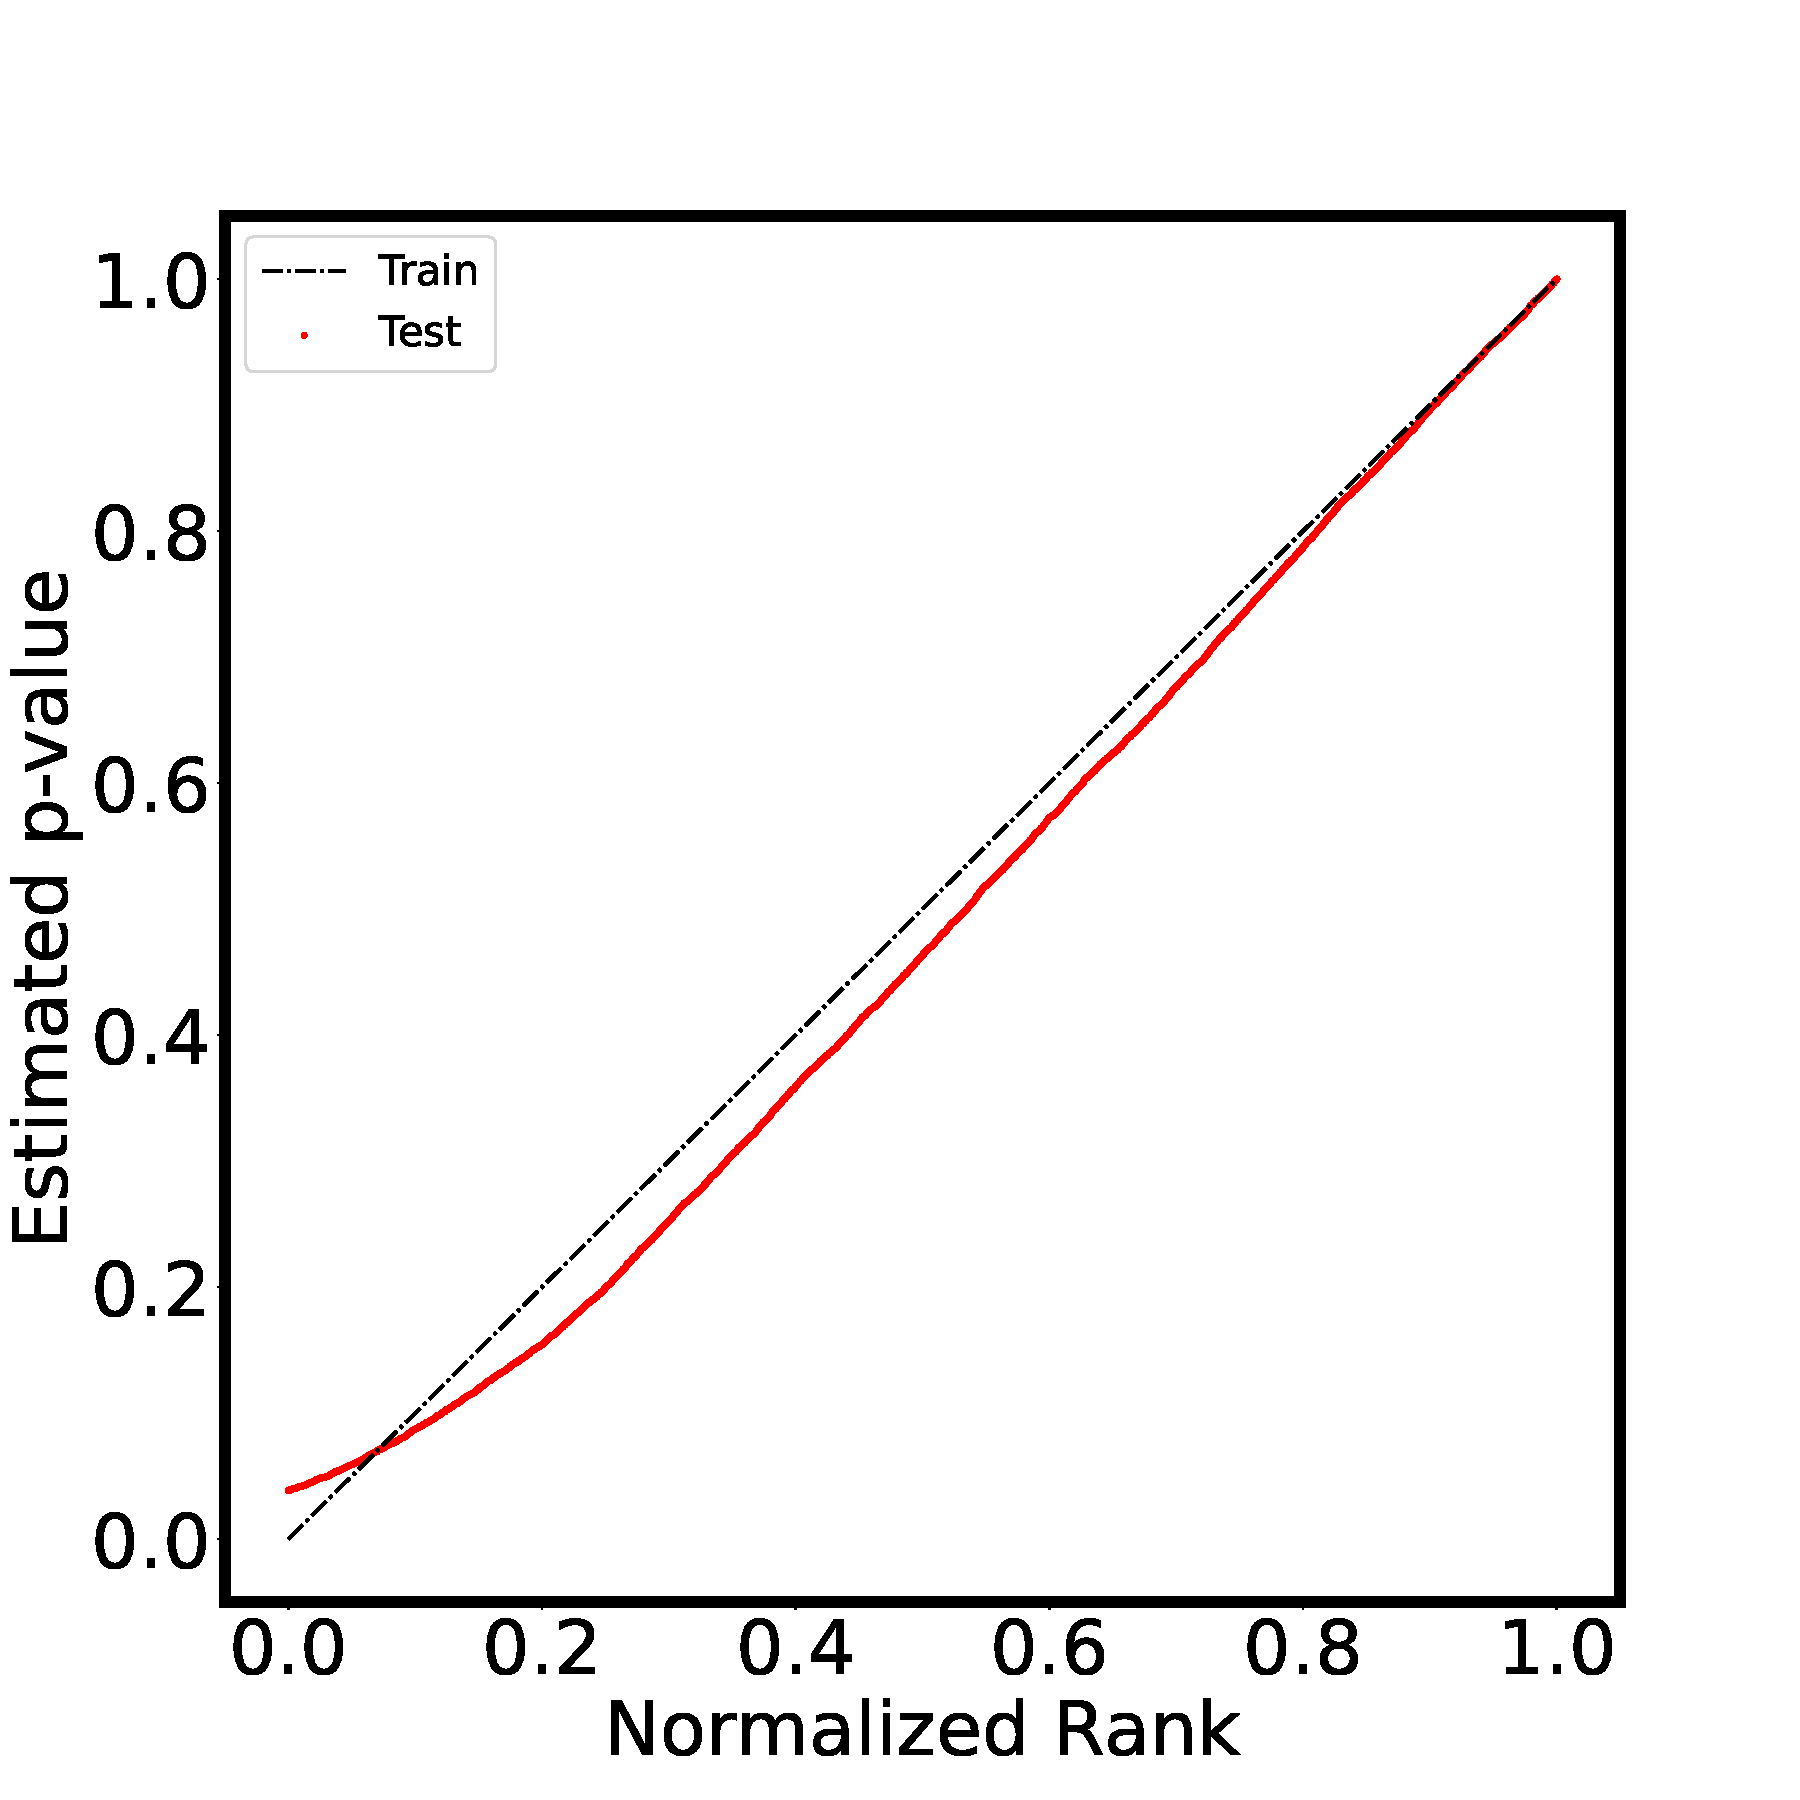
\includegraphics[width=2.5in]{img/pcam_QQ.pdf} &
		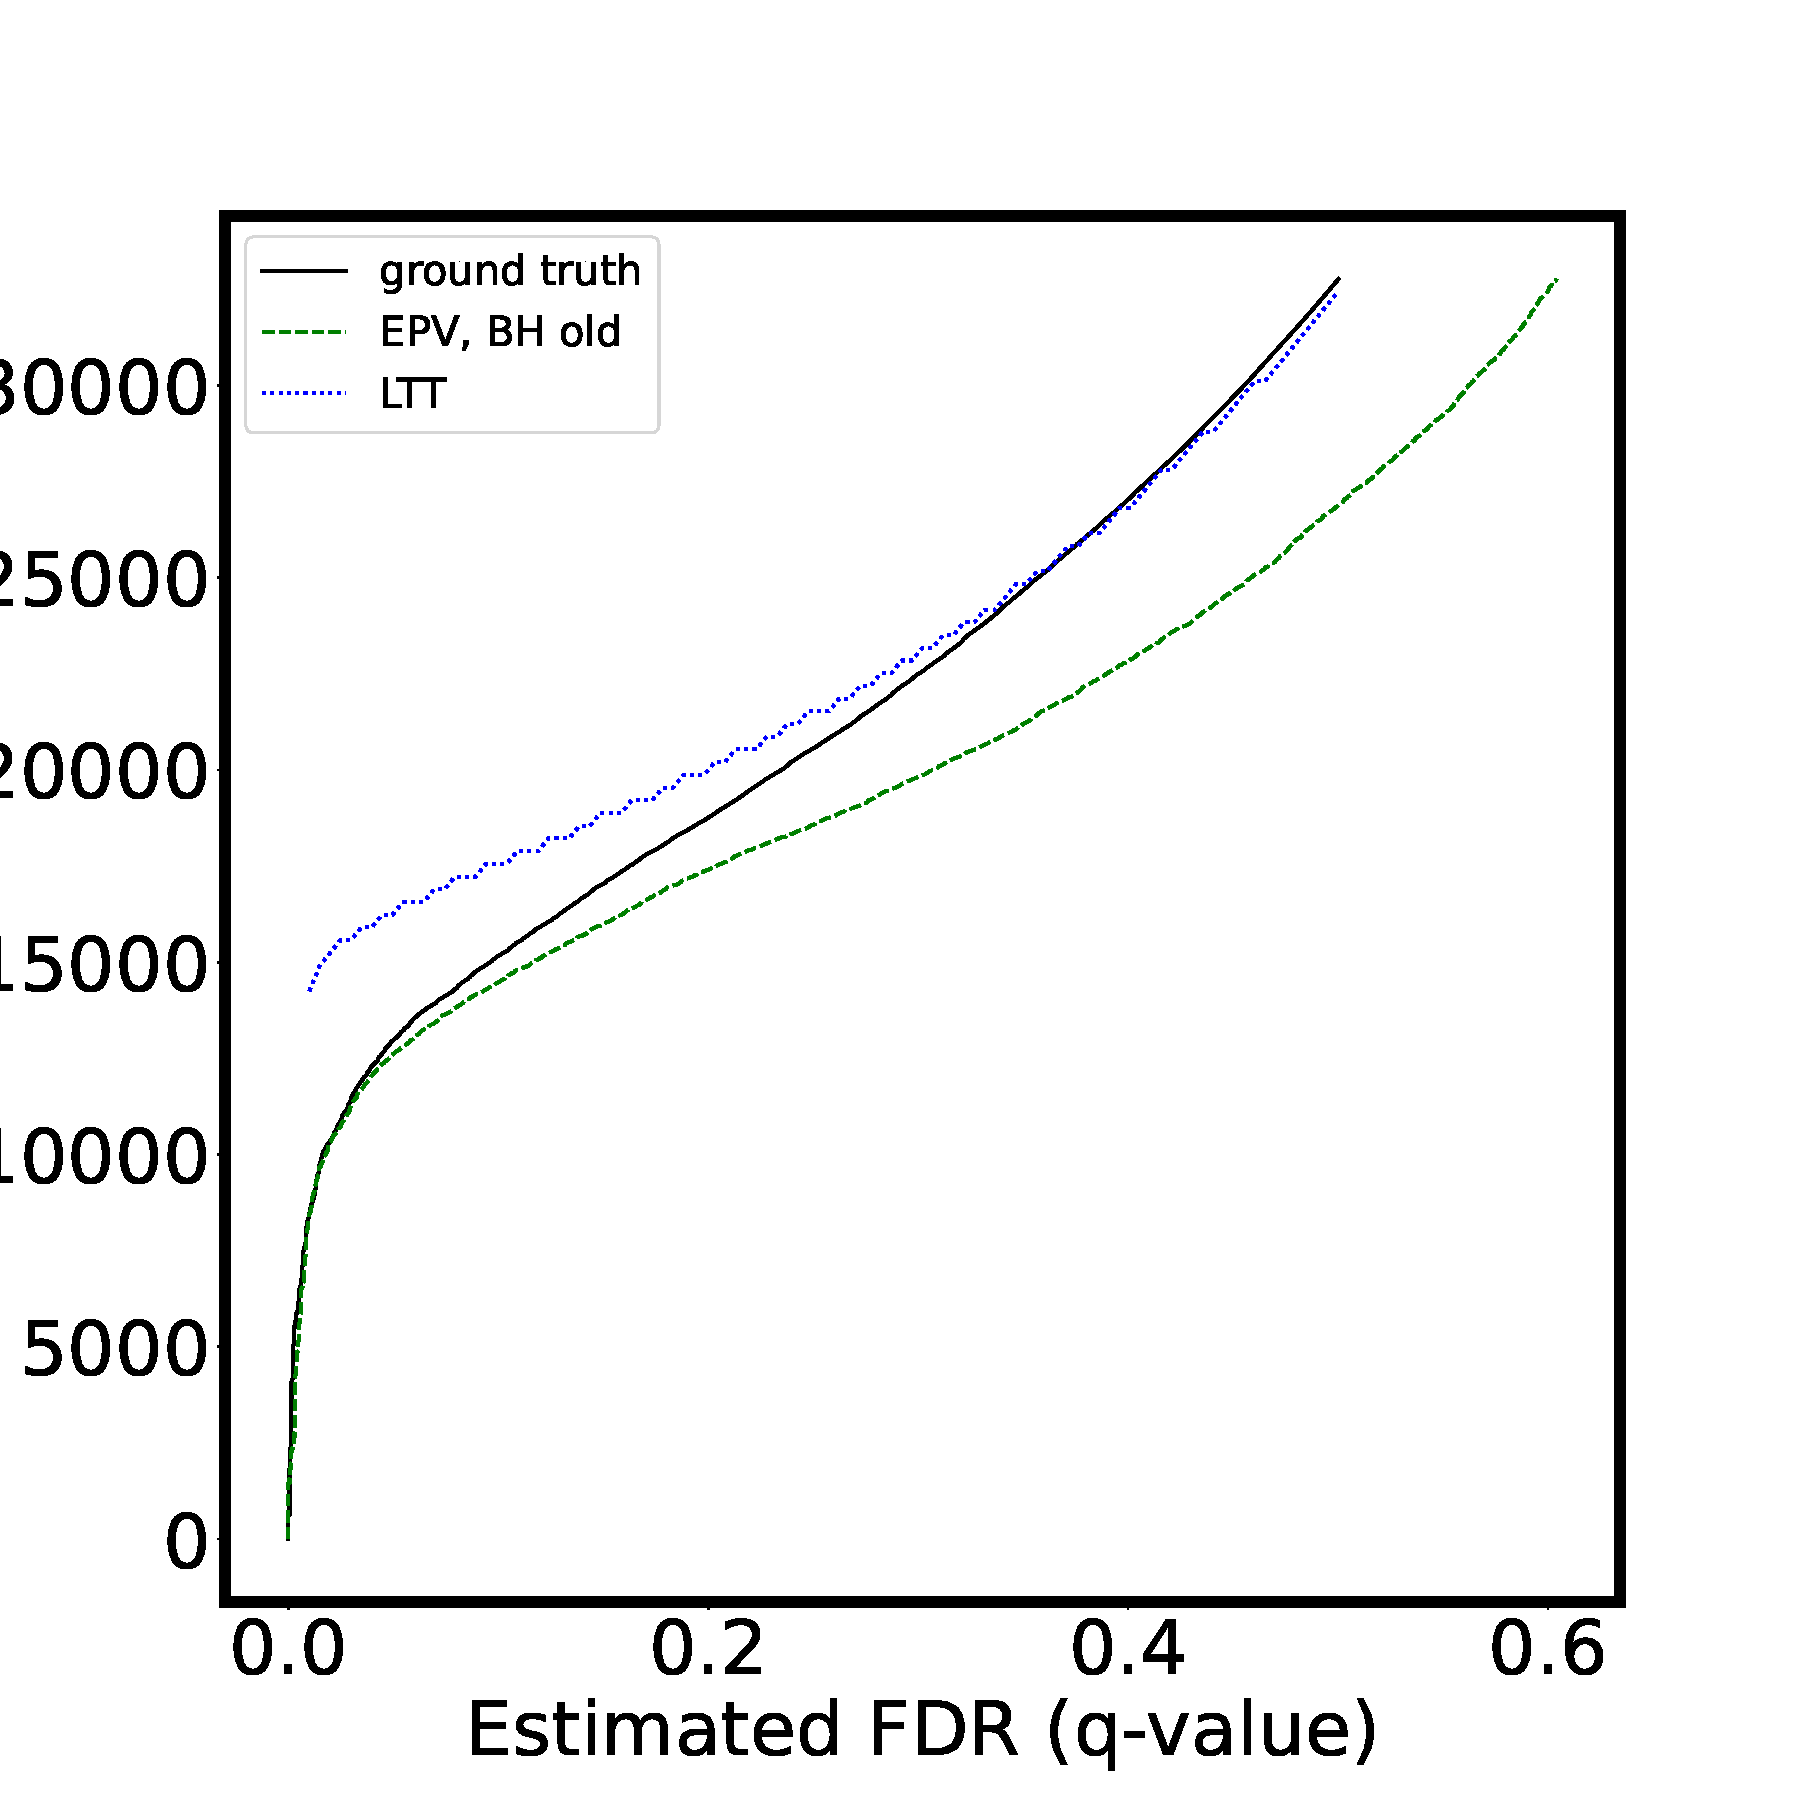
\includegraphics[width=2.5in]{img/pcam_fdr_control.pdf} & 
            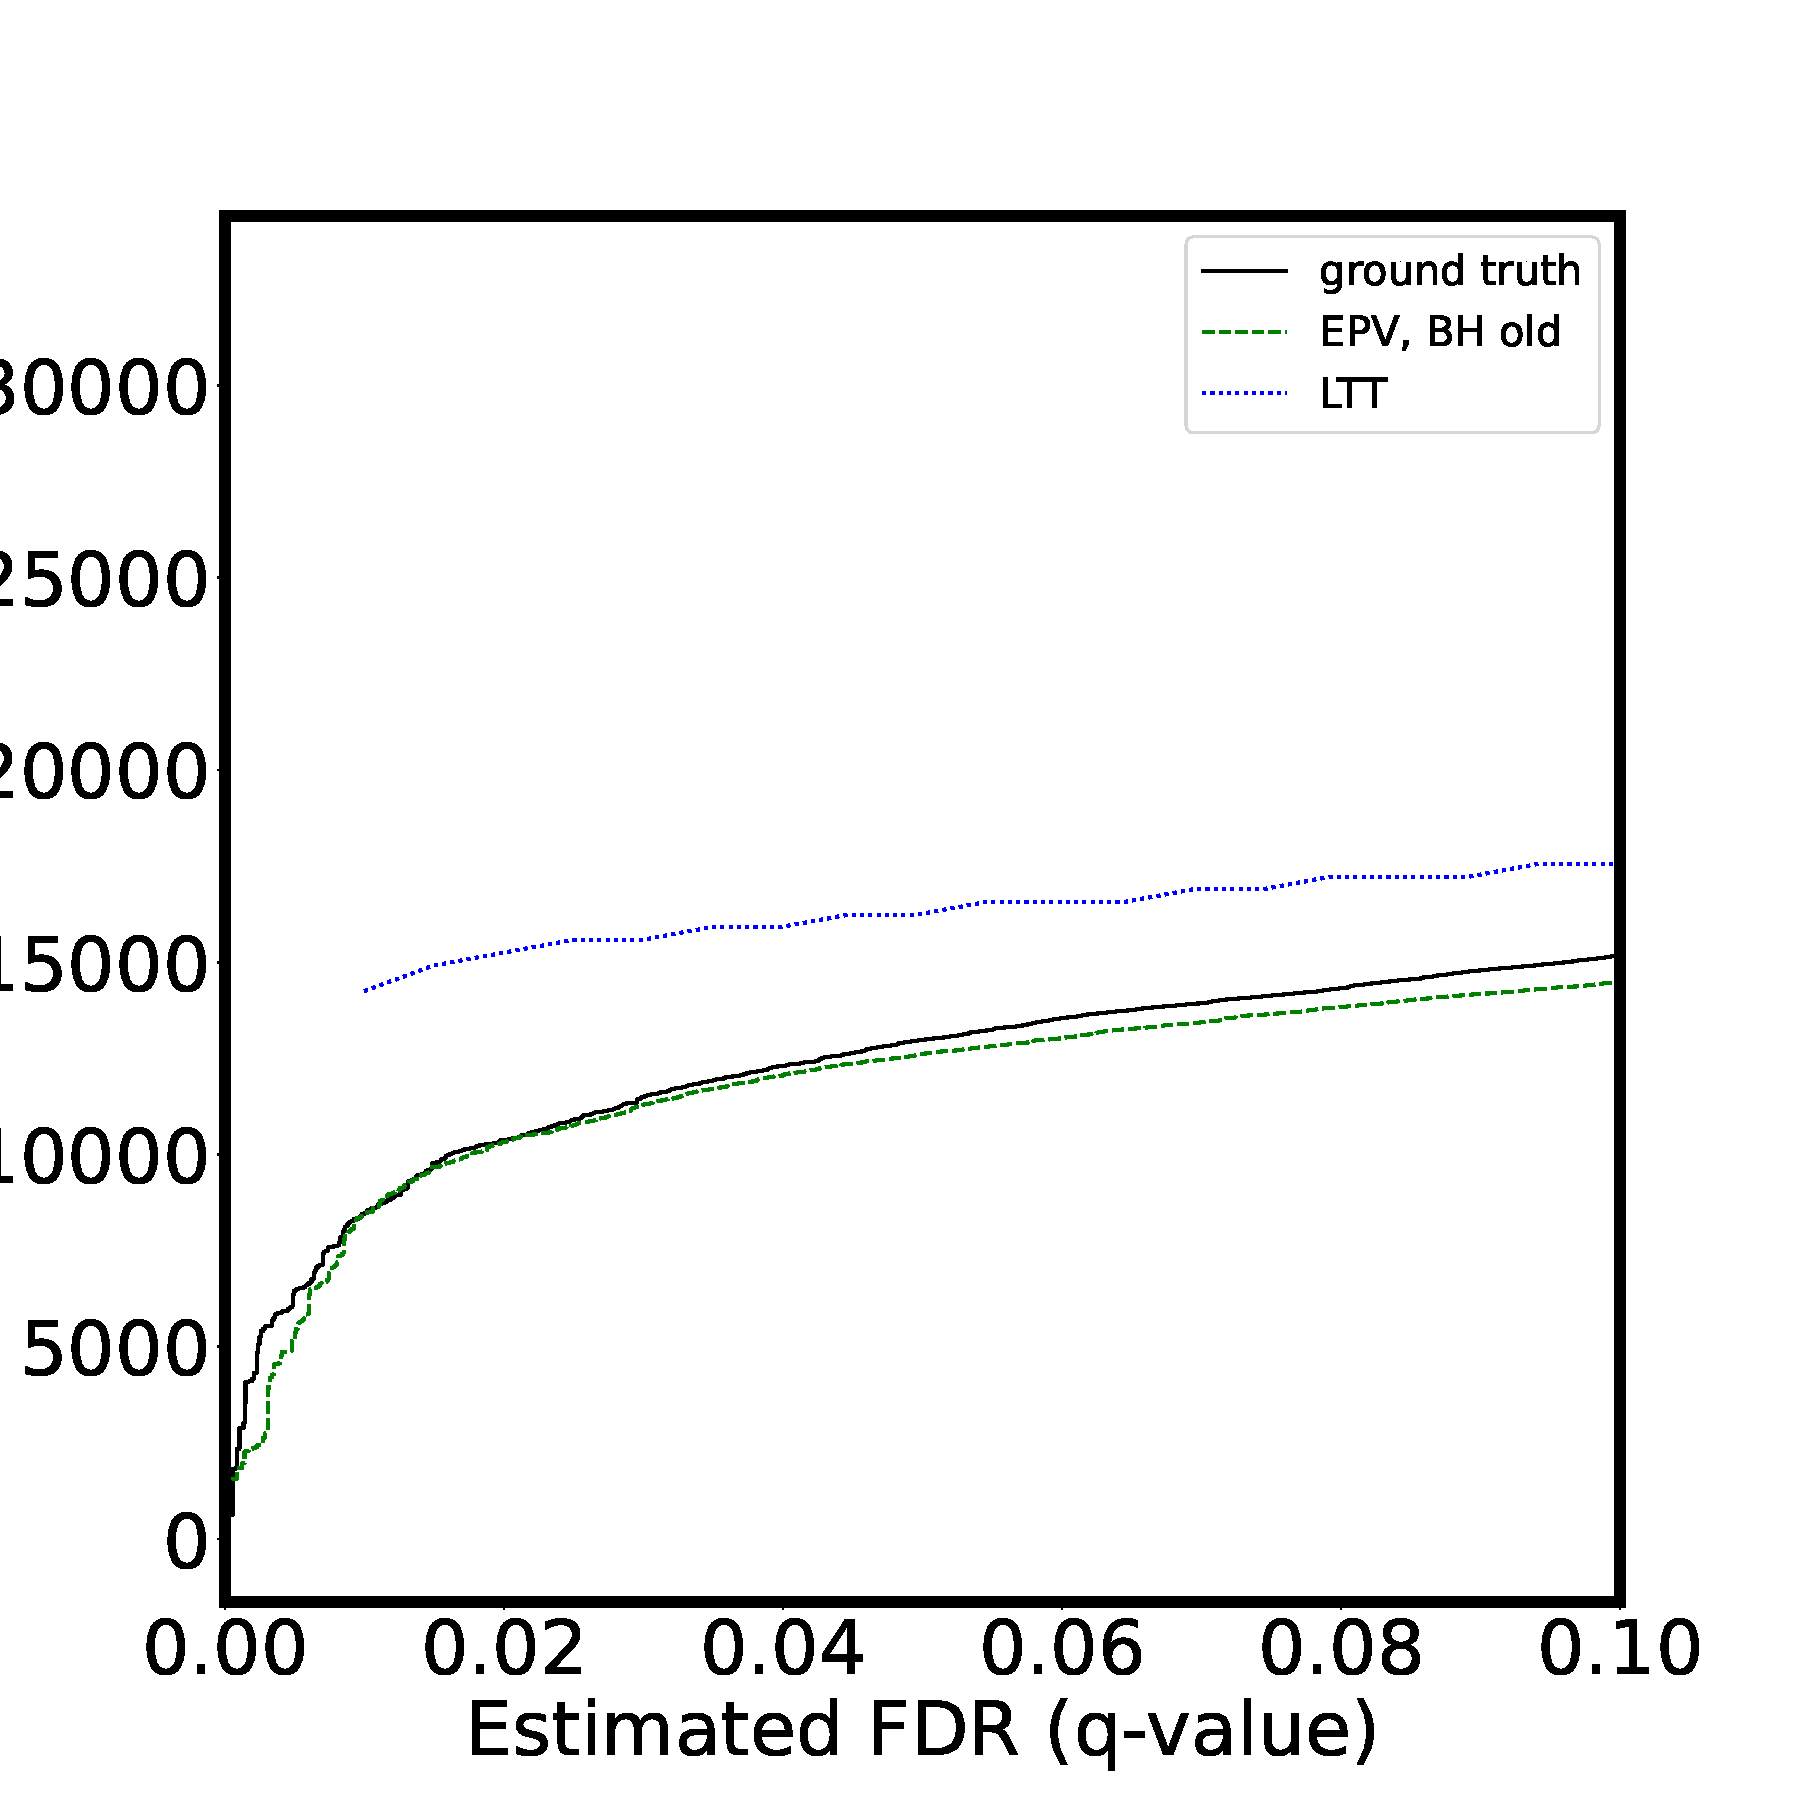
\includegraphics[width=2.5in]{img/pcam_fdr_control_loc.pdf}
		\\	
		A & B & C
	\end{tabular}
	\caption{\bf FDR control with p-values for PCam dataset.}
	\label{fig:pcam}
\end{figure} 

\subsubsection{Rebalanced case}

\begin{figure}
	\advance\leftskip-0.5cm
	\begin{tabular}{ccc}
 		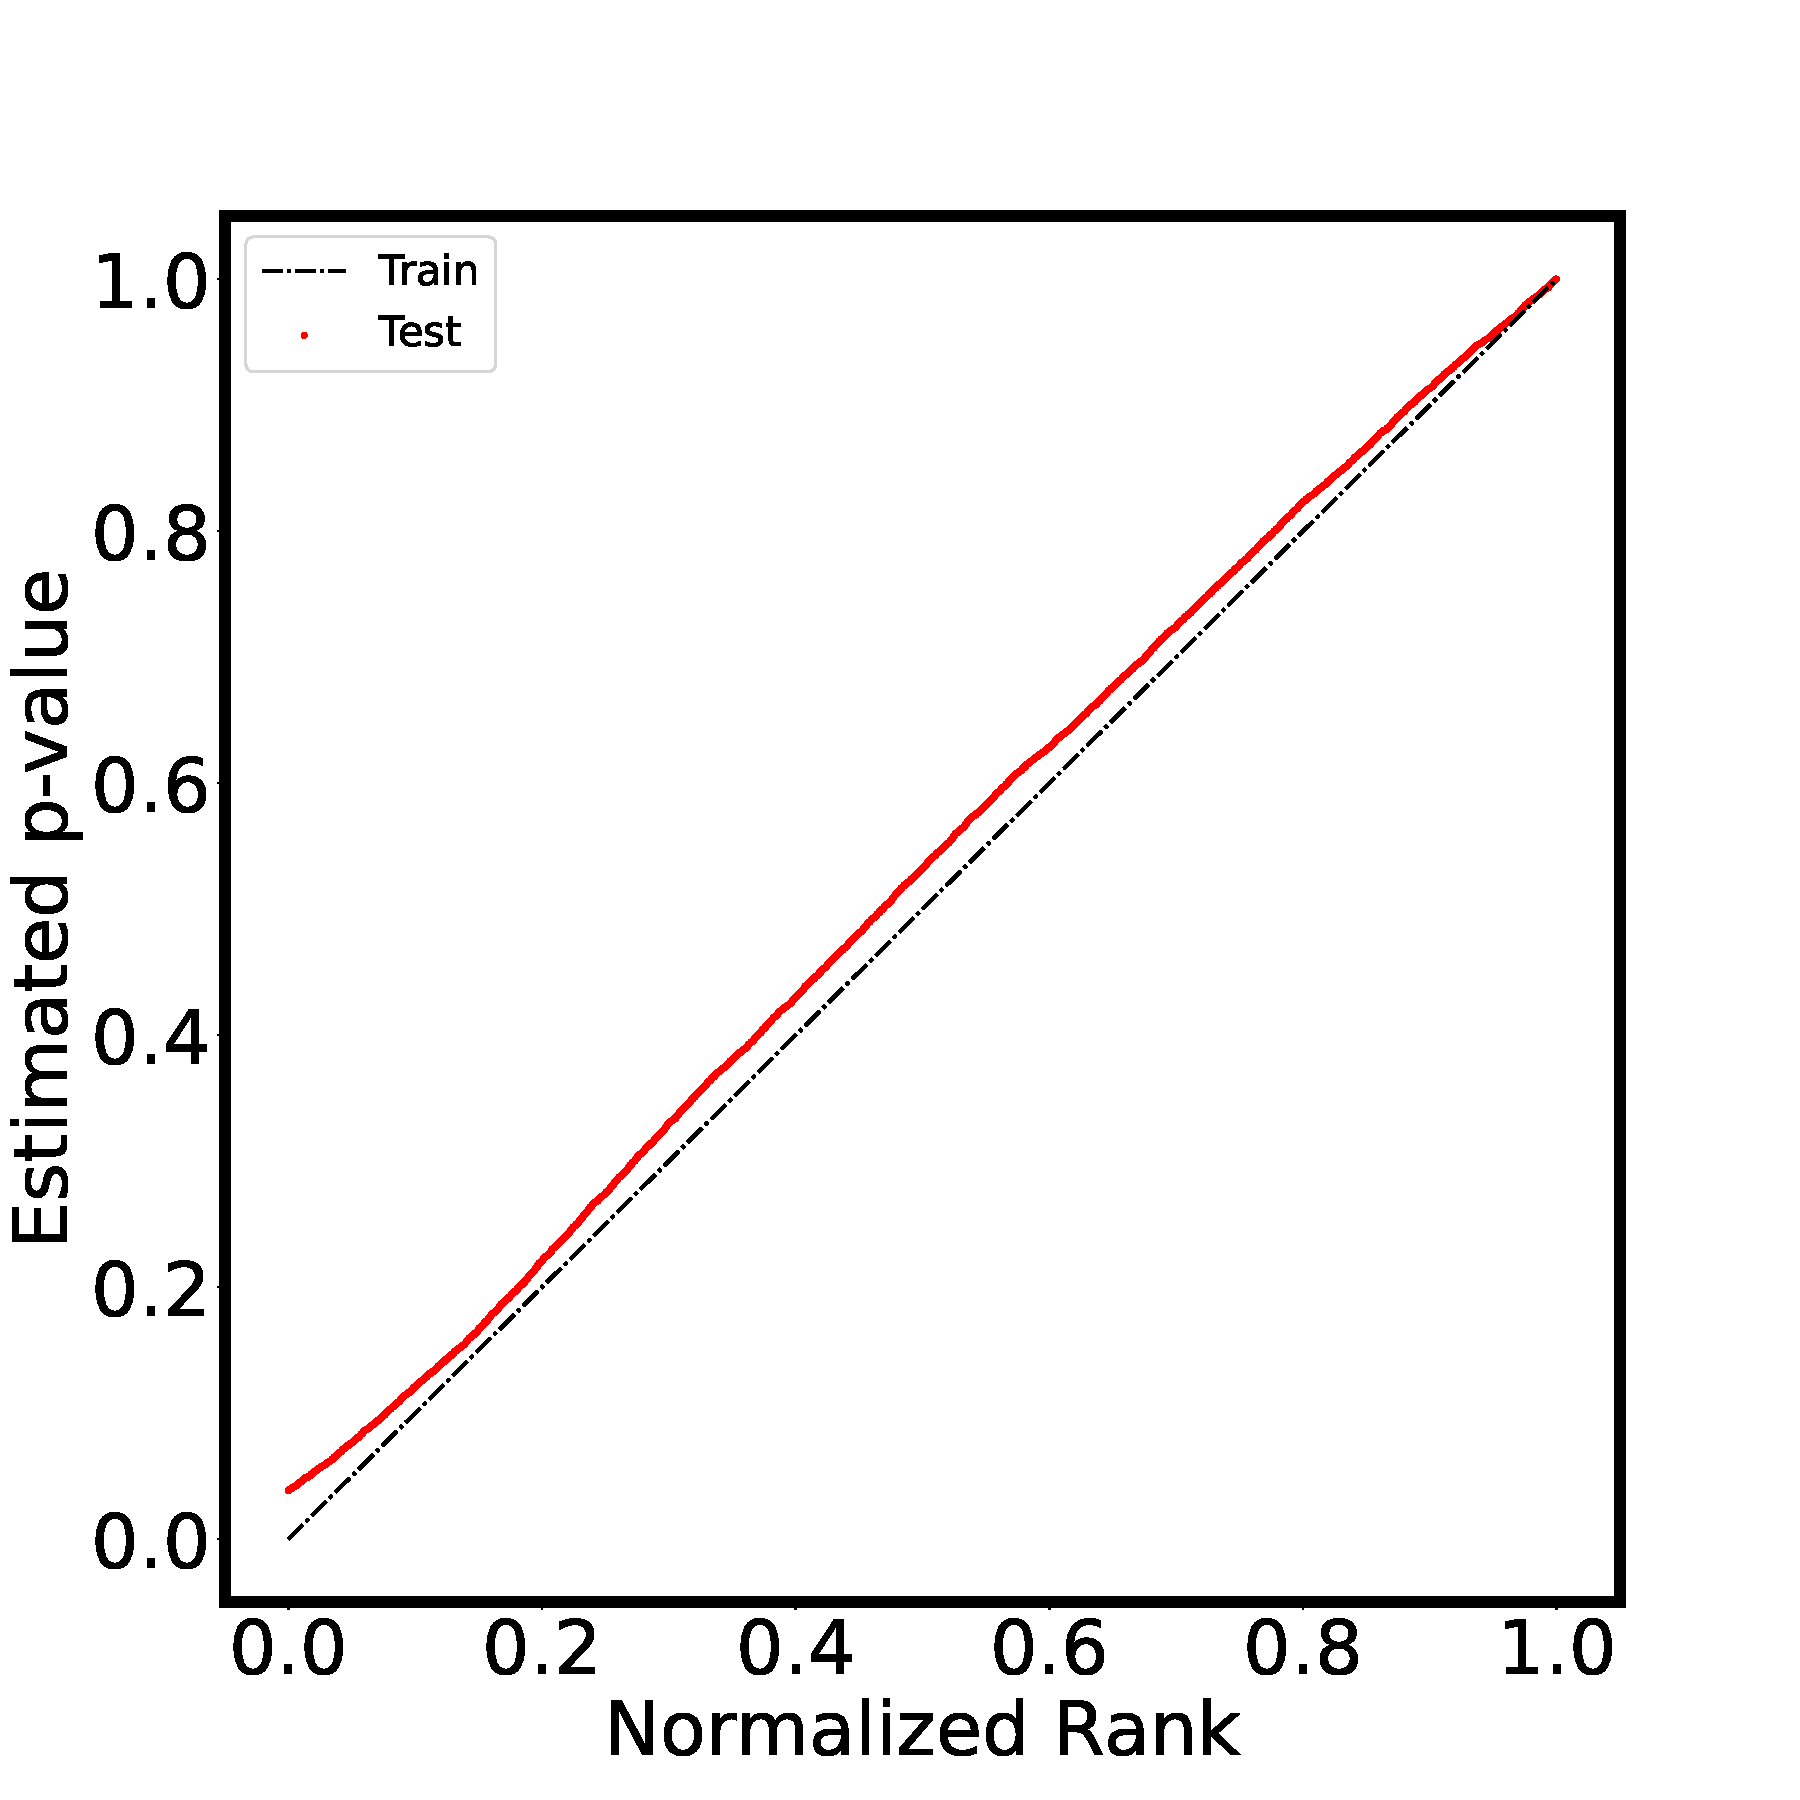
\includegraphics[width=2.5in]{img/pcam_balanced_QQ.pdf} &
		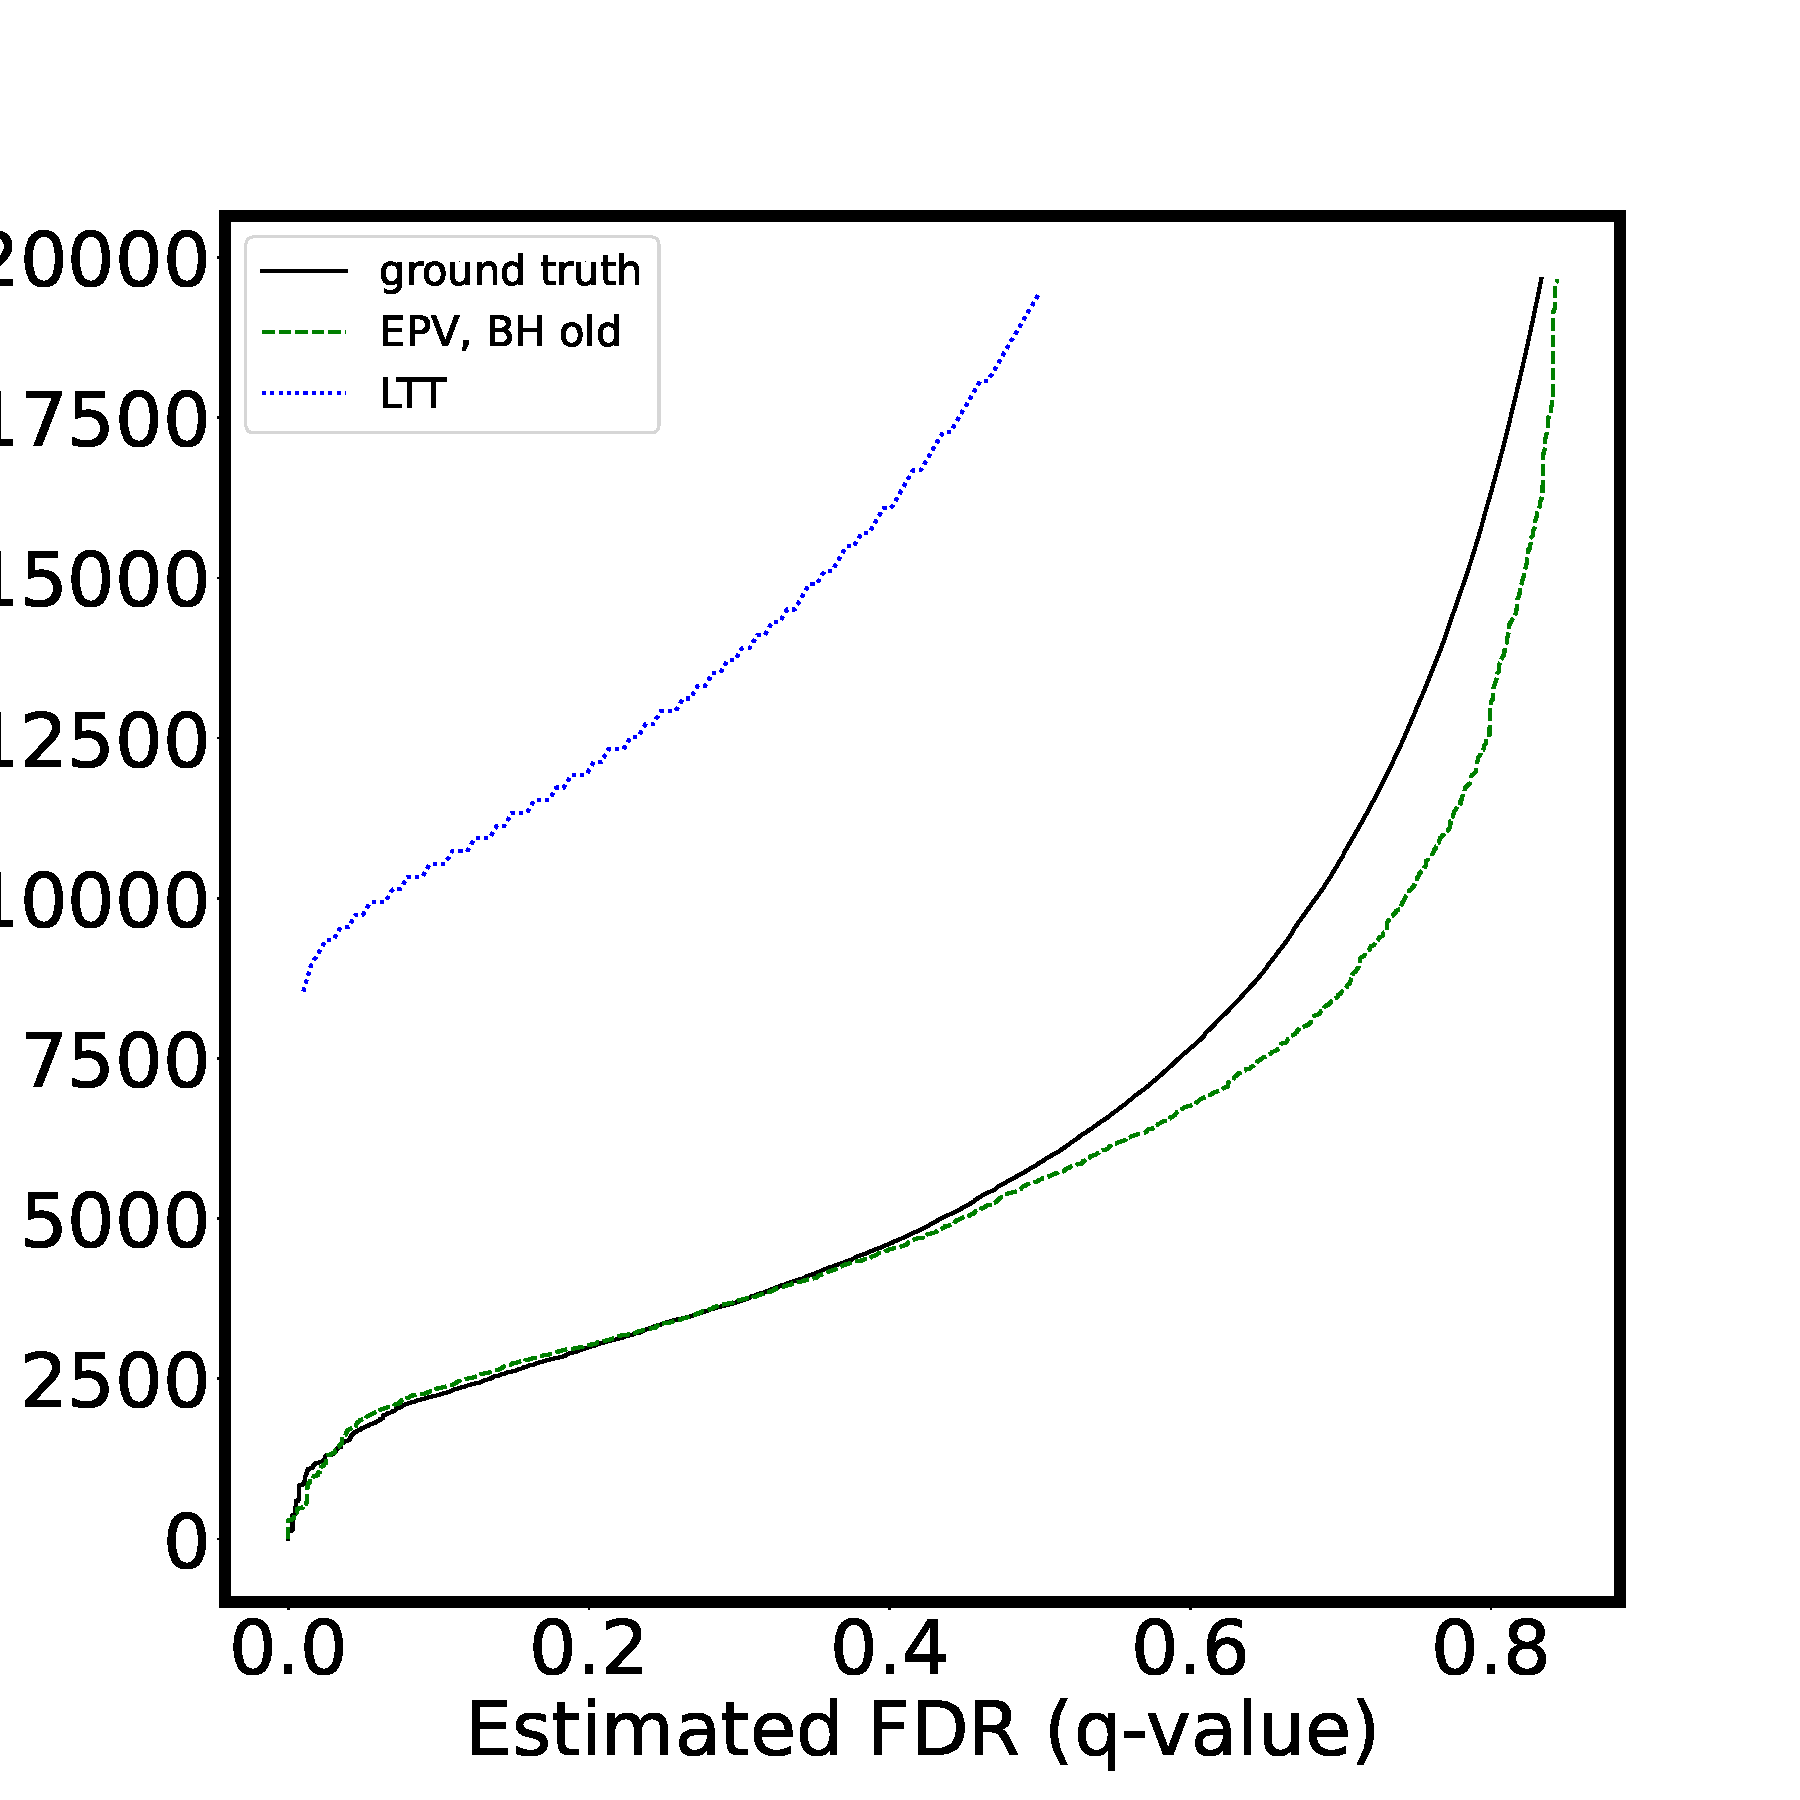
\includegraphics[width=2.5in]{img/pcam_balanced_fdr_control.pdf} & 
            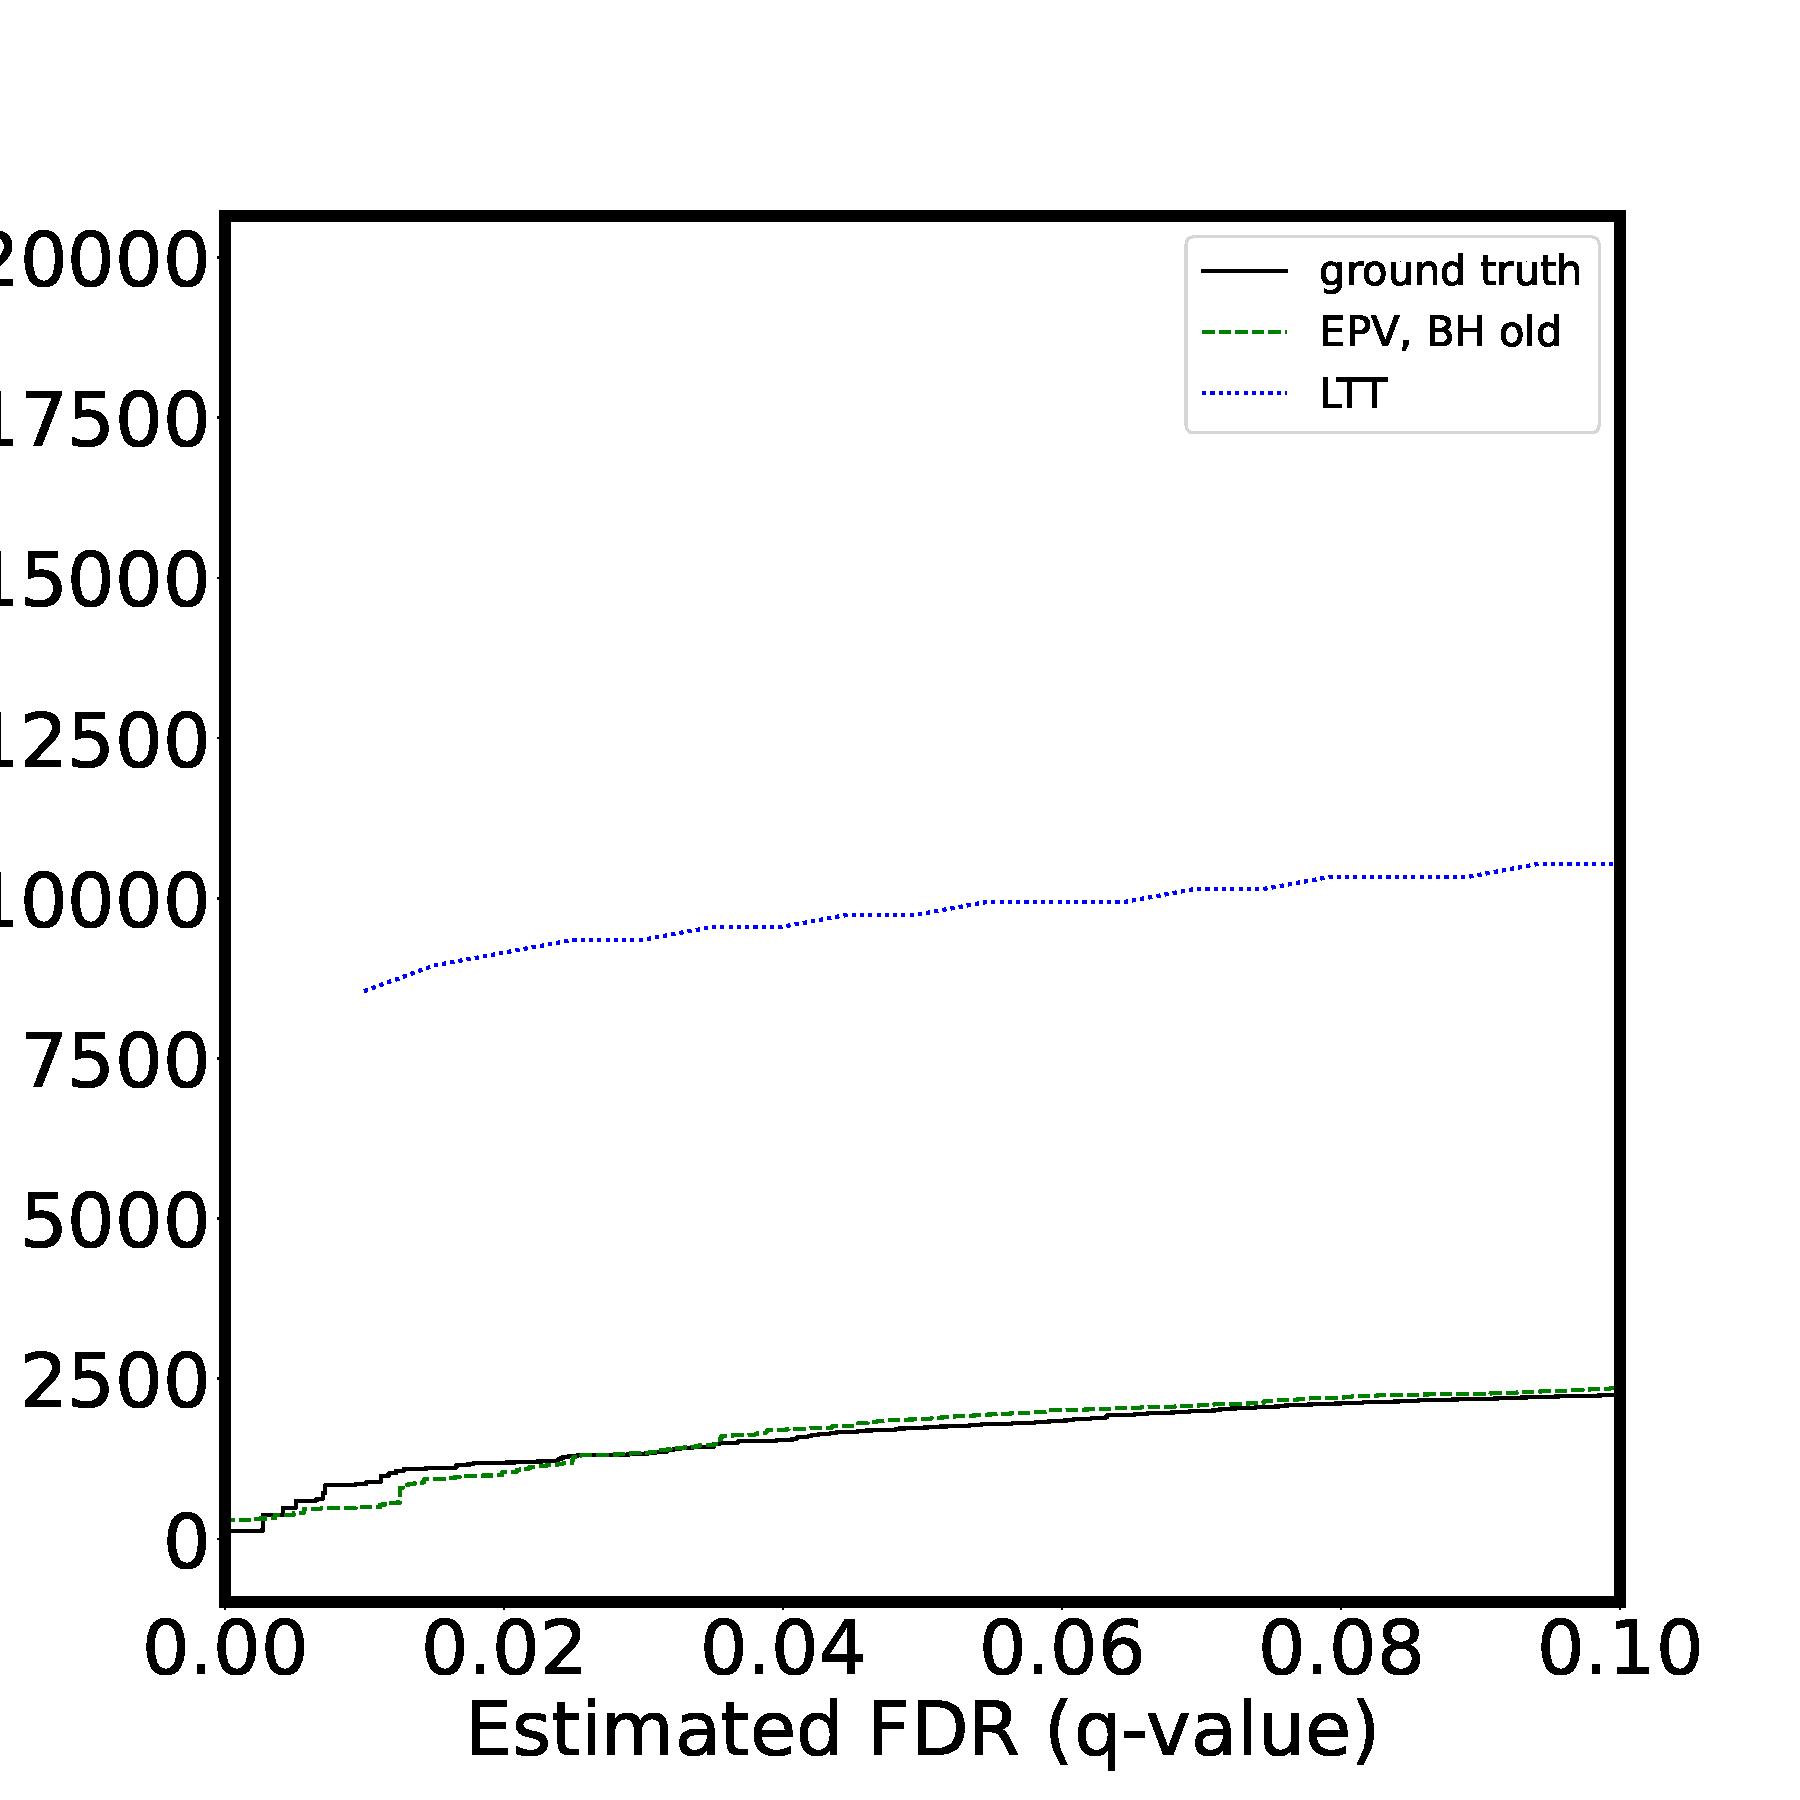
\includegraphics[width=2.5in]{img/pcam_balanced_fdr_control_loc.pdf}
		\\	
		A & B & C
	\end{tabular}
	\caption{\bf FDR control with p-values for rebalanced PCam dataset.}
	\label{fig:pcam}
\end{figure} 

\subsection{Biomedical data: cells segmentation}

\begin{figure}
	\advance\leftskip-0.5cm
	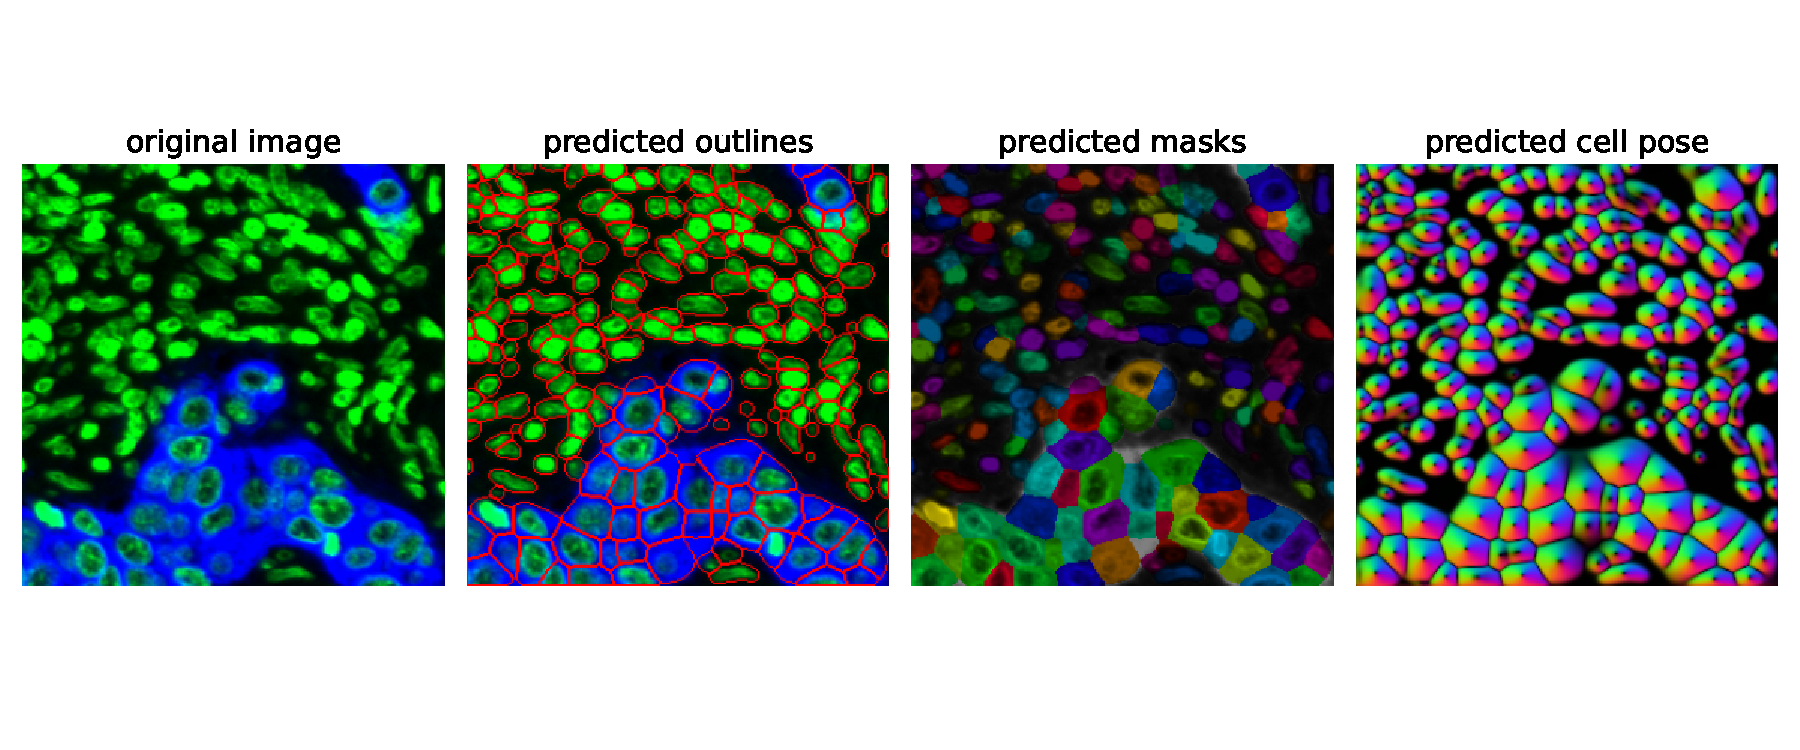
\includegraphics[width=8in]{img/tissuenet.pdf}
	\caption{{\bf Instance of TissueNet dataset.} Two-channel original images are being processed by the model, in turn producing masks \& flows to correctly segment cells}
	\label{fig:tissue_example}
\end{figure} 

\subsubsection{Datasets and Models}

TissueNet dataset is introduced as a new word in pixel-level segmentation task, declaring more than 1.3 million manually labeled and paired whole-cell and nuclear annotations. Outperforming any rival collection of data in this field, TissueNet was constructed through a multi-stage human-in-the-loop approach. It contains (512, 512) images from six various platforms and nine organs, all implying inclusion of both histologically healthy and diseased tissues. In total, there are 13 distinct classes presented. However, we do transform the task towards binary identification of the null class, simply striving to disassociate each cell.   

The embodied model is derived from the Cellpose 2.0 package. It suggests an ensemble of numerous  pretrained models joined with human-in-the-loop pipeline. Together, they allow to easily fine-tune the particular model for any cell segmentation dataset.

\subsubsection{Standard case}

\begin{figure}
	\centering
	\begin{tabular}{ccc}
 		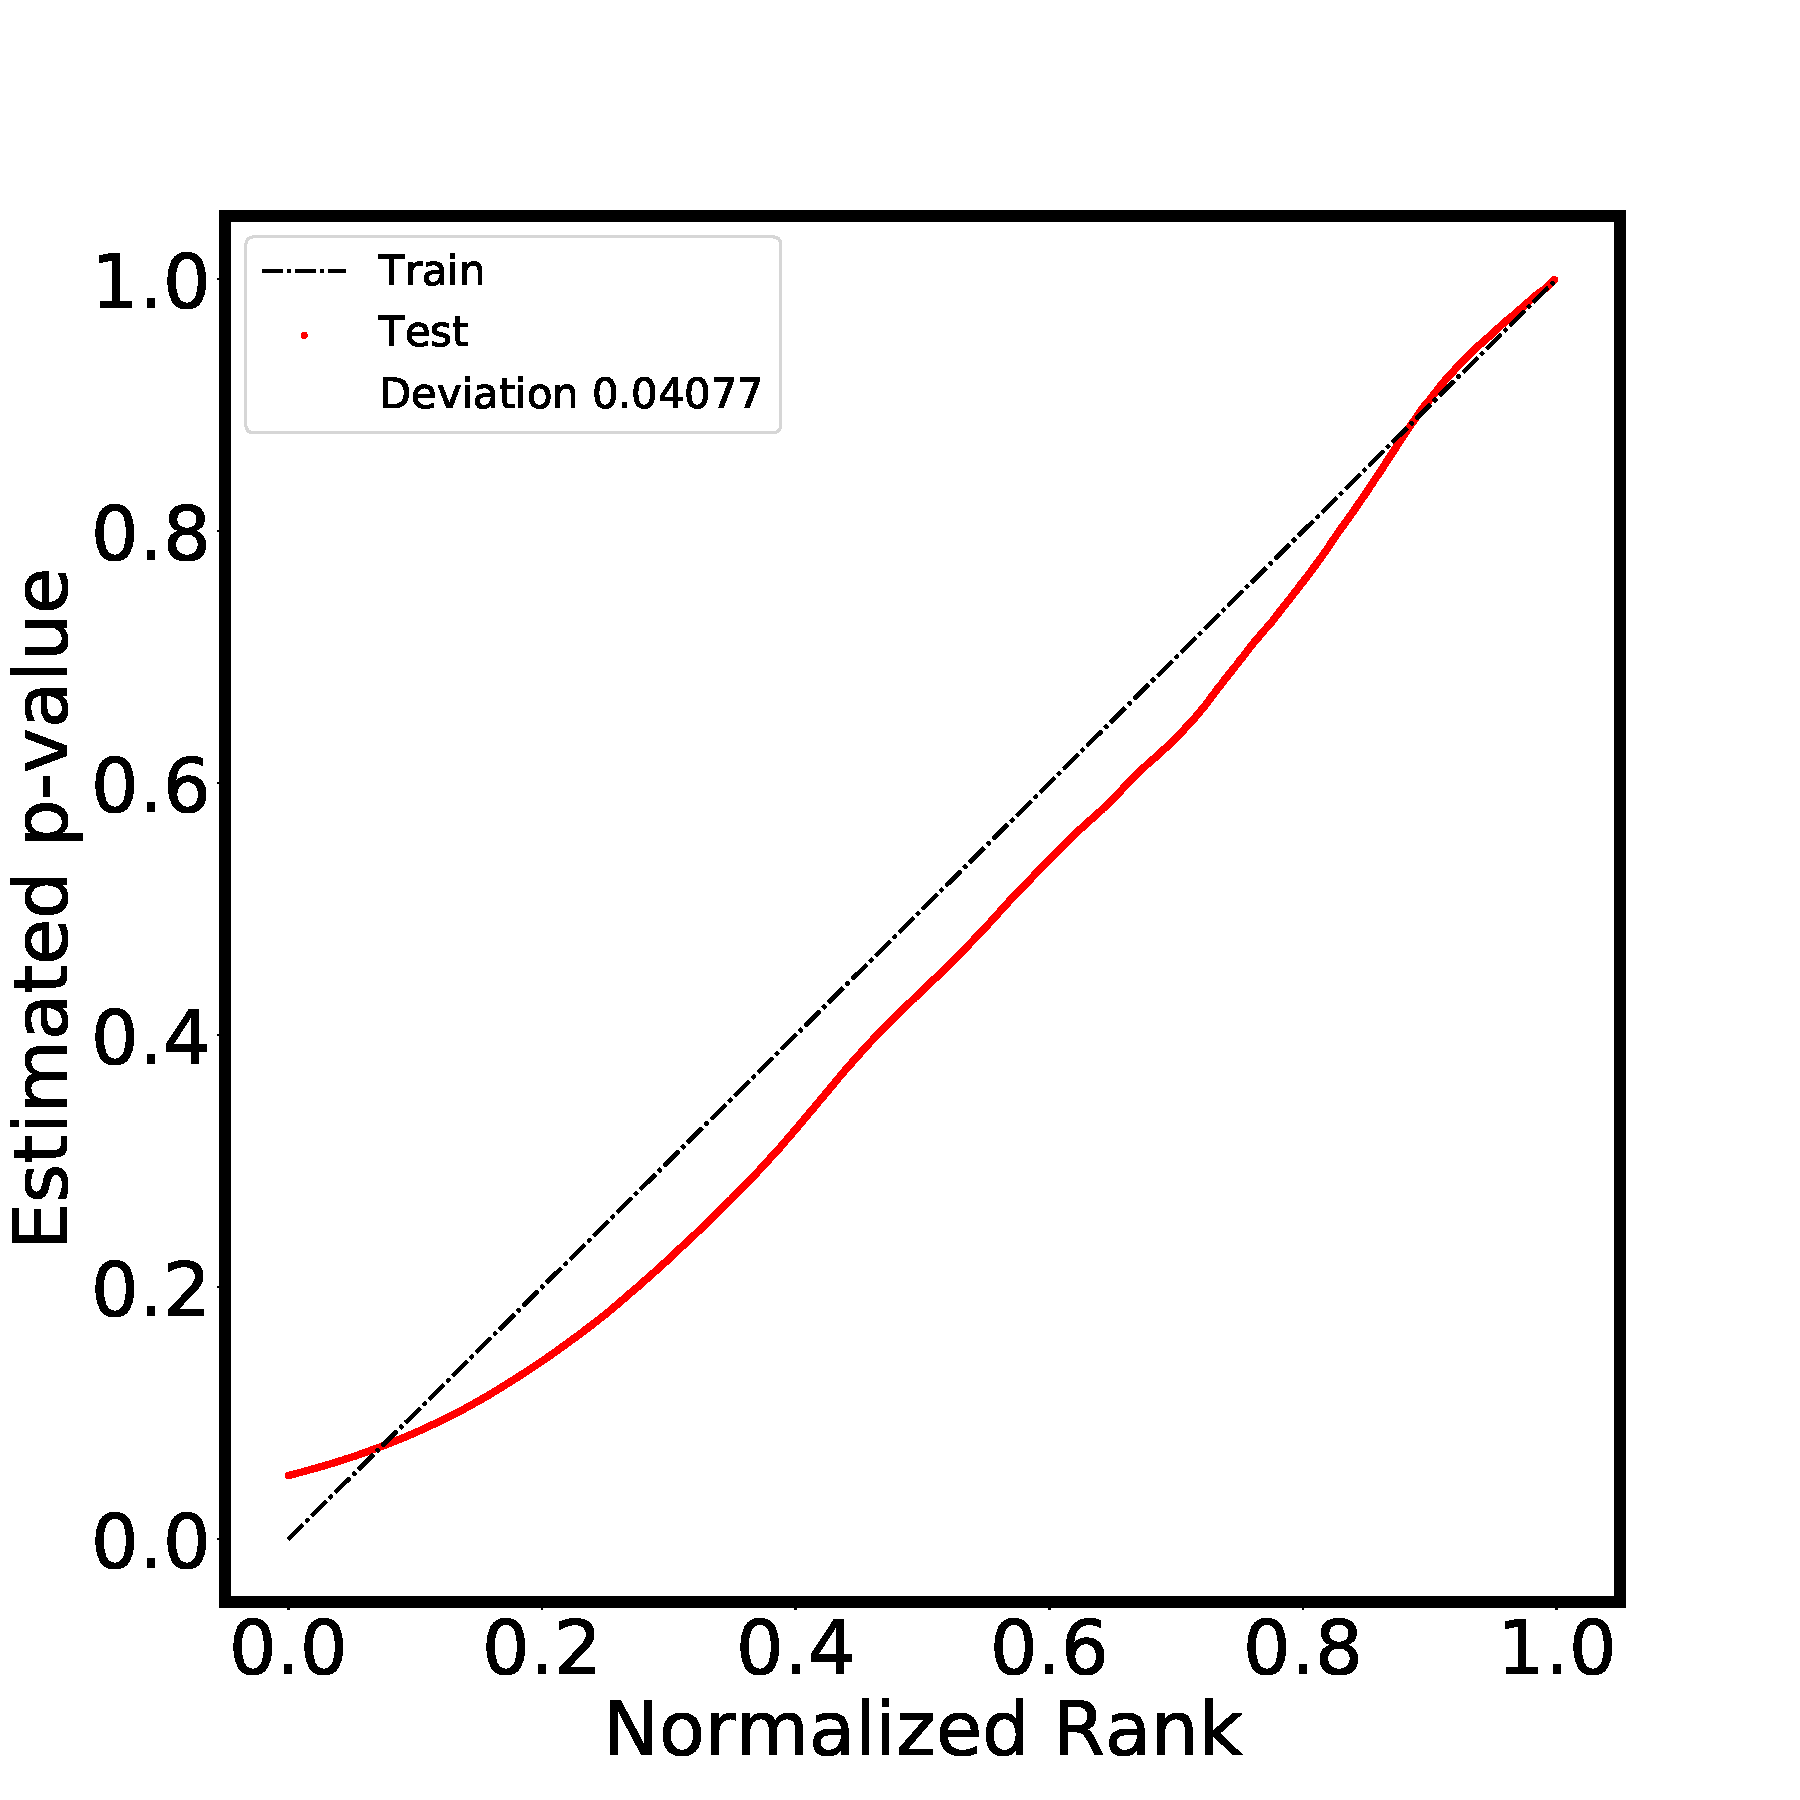
\includegraphics[width=2in]{img/segment_cls_QQ.pdf} &
		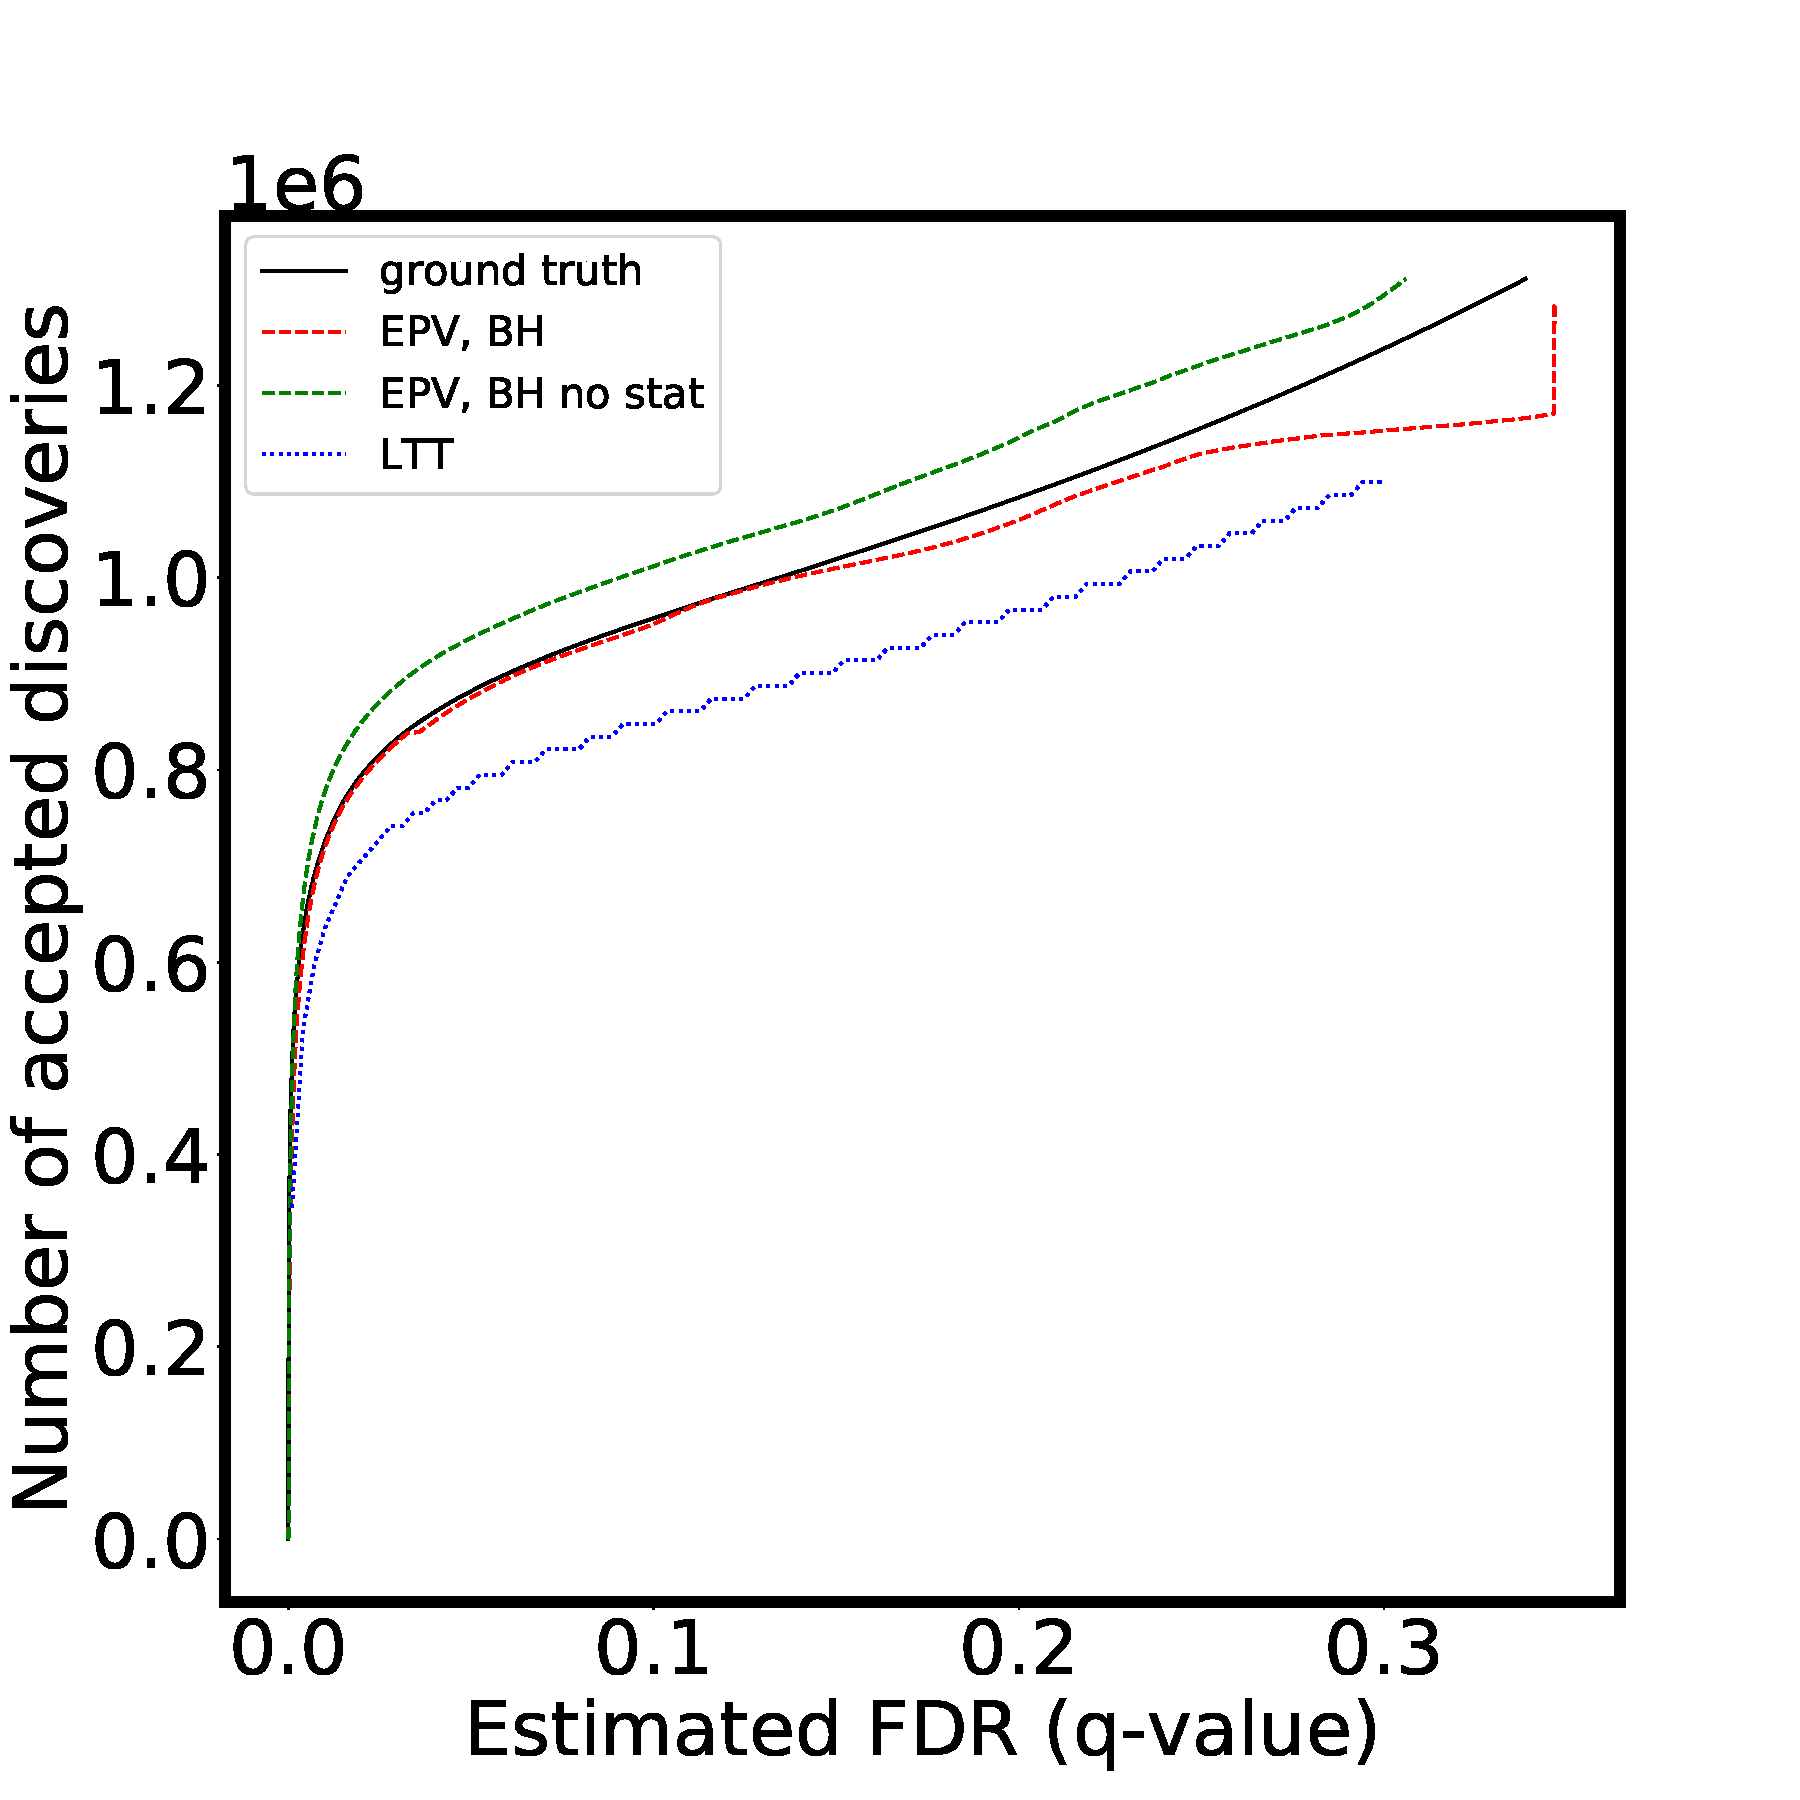
\includegraphics[width=2in]{img/segment_cls_fdr_control.pdf} & 
            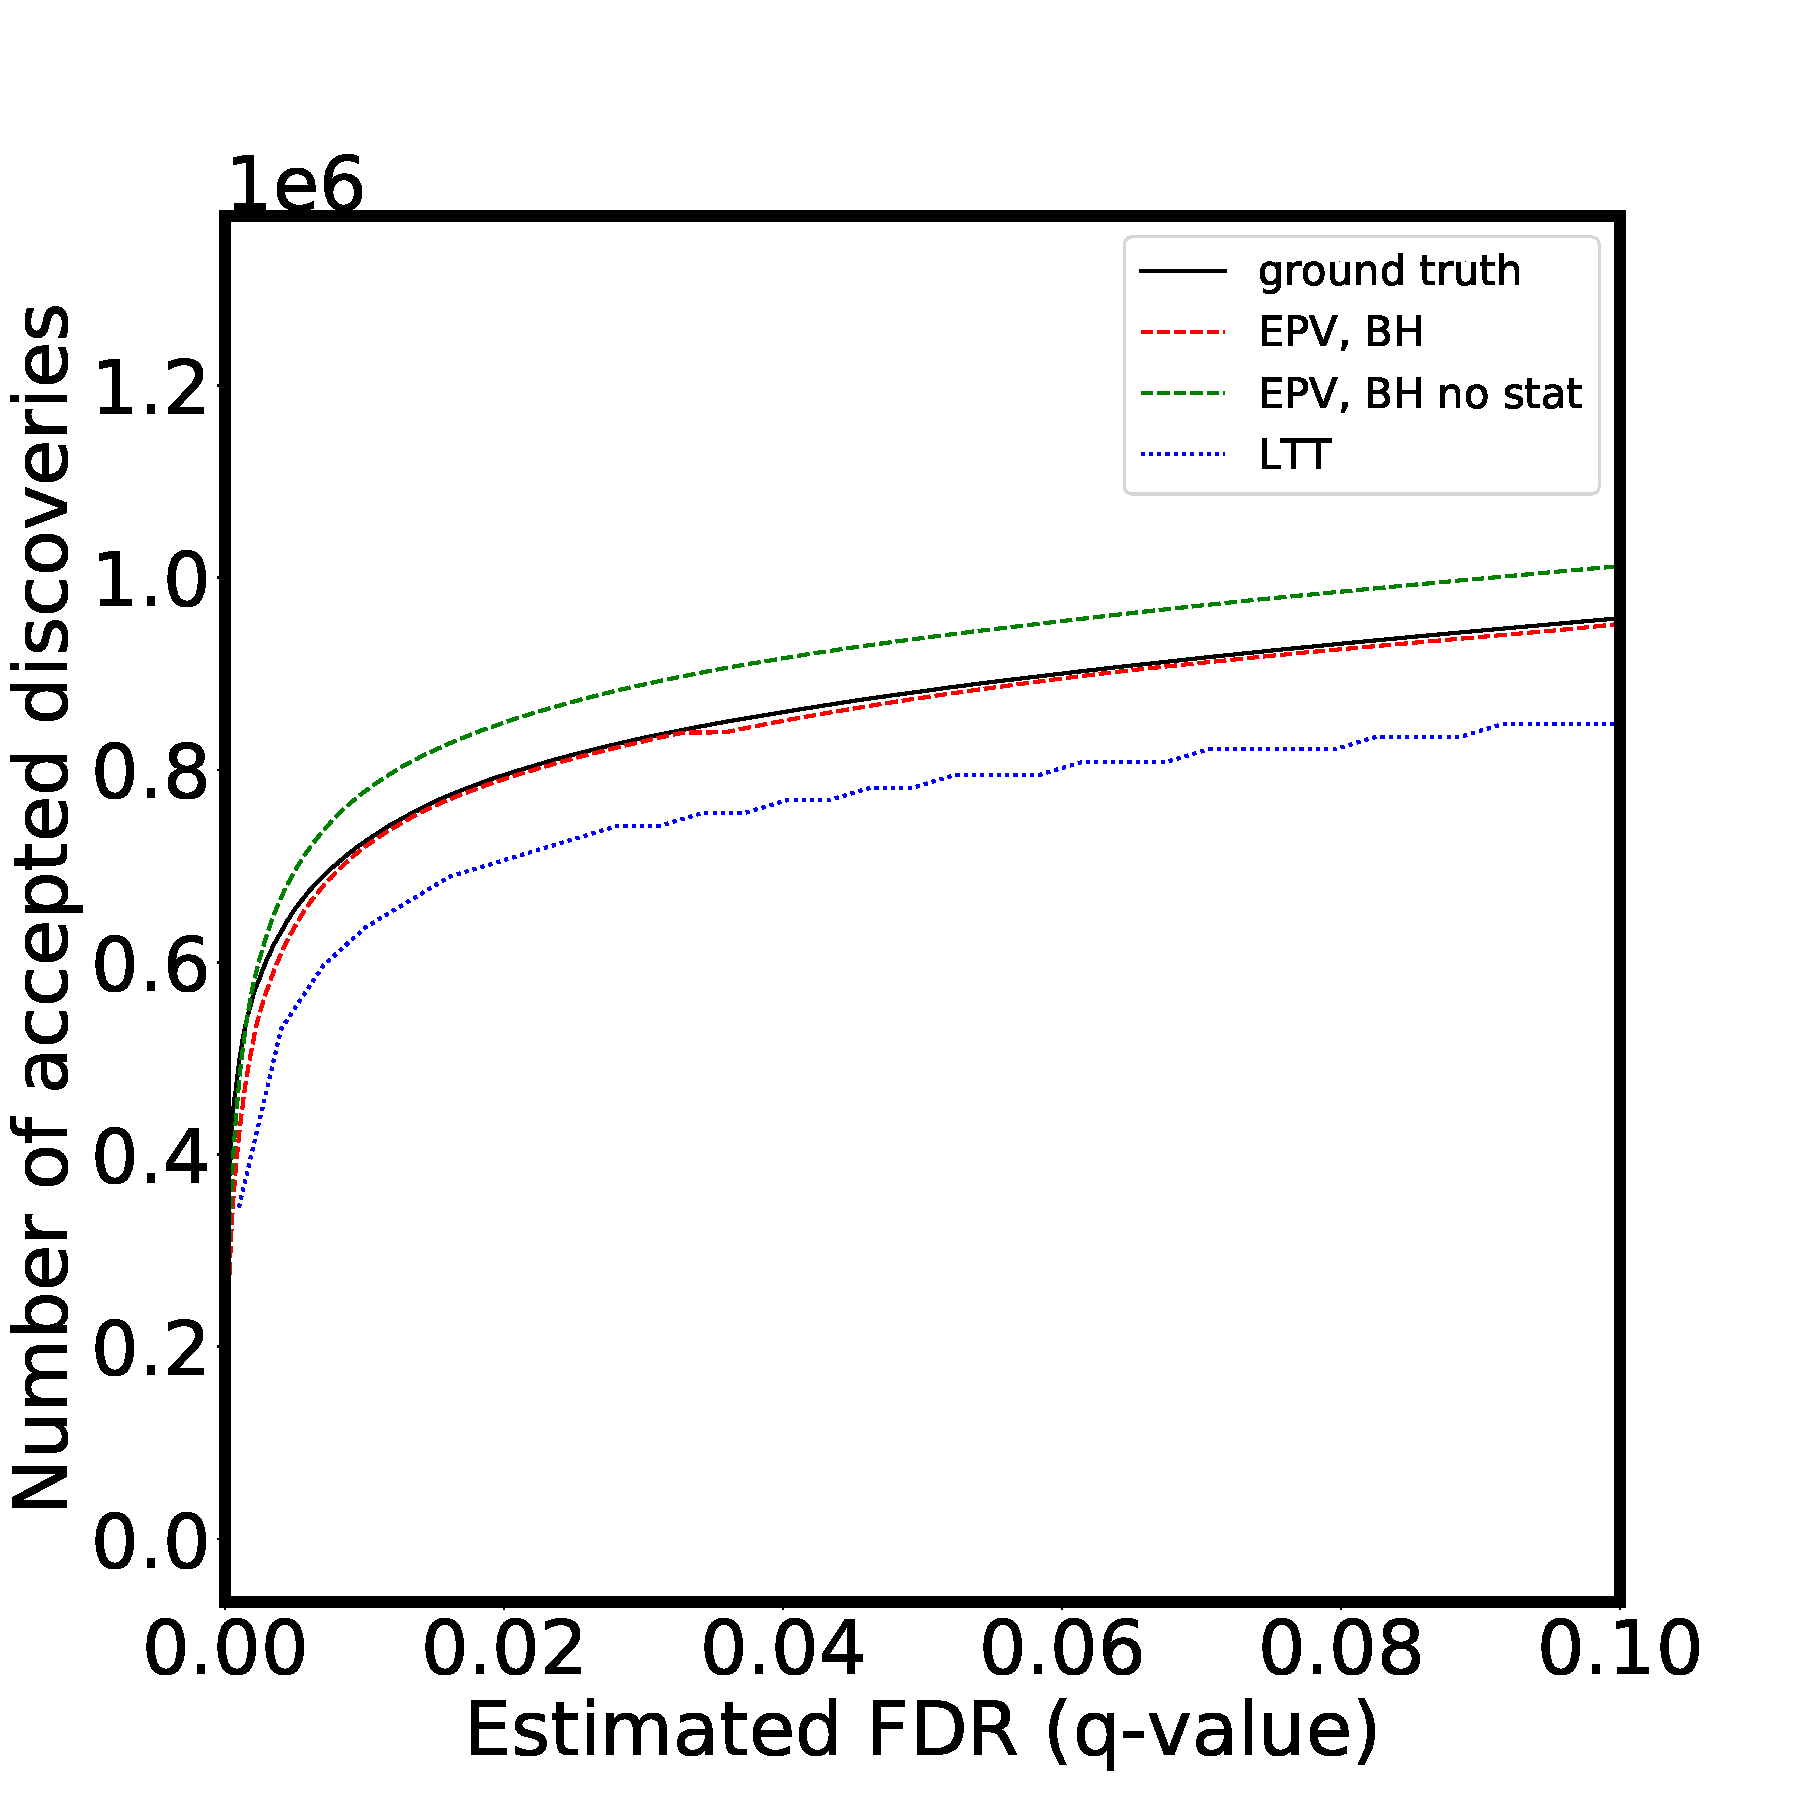
\includegraphics[width=2in]{img/segment_cls_fdr_control_loc.pdf}
		\\	
		A & B & C
	\end{tabular}
	\caption{\bf FDR control with p-values for TissueNet dataset.}
	\label{fig:pcam}
\end{figure}

\subsection{Loan exposure data}

\subsubsection{Datasets and Models}

\subsubsection{Standard case}


\begin{figure}
	\centering
	\begin{tabular}{ccc}
 		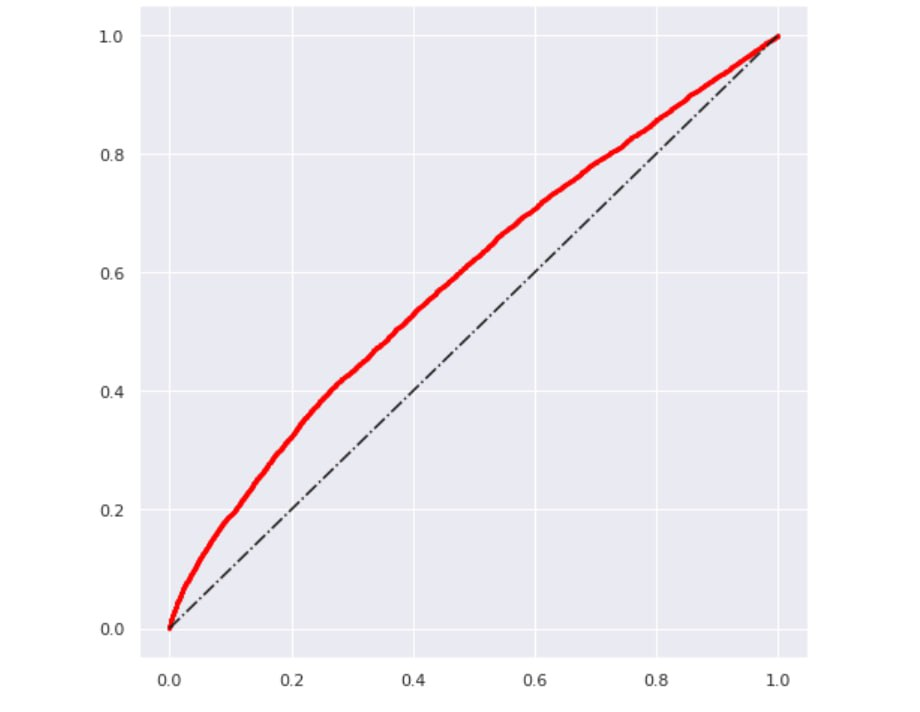
\includegraphics[width=2in]{img/tinkoff_QQ.jpeg} &
		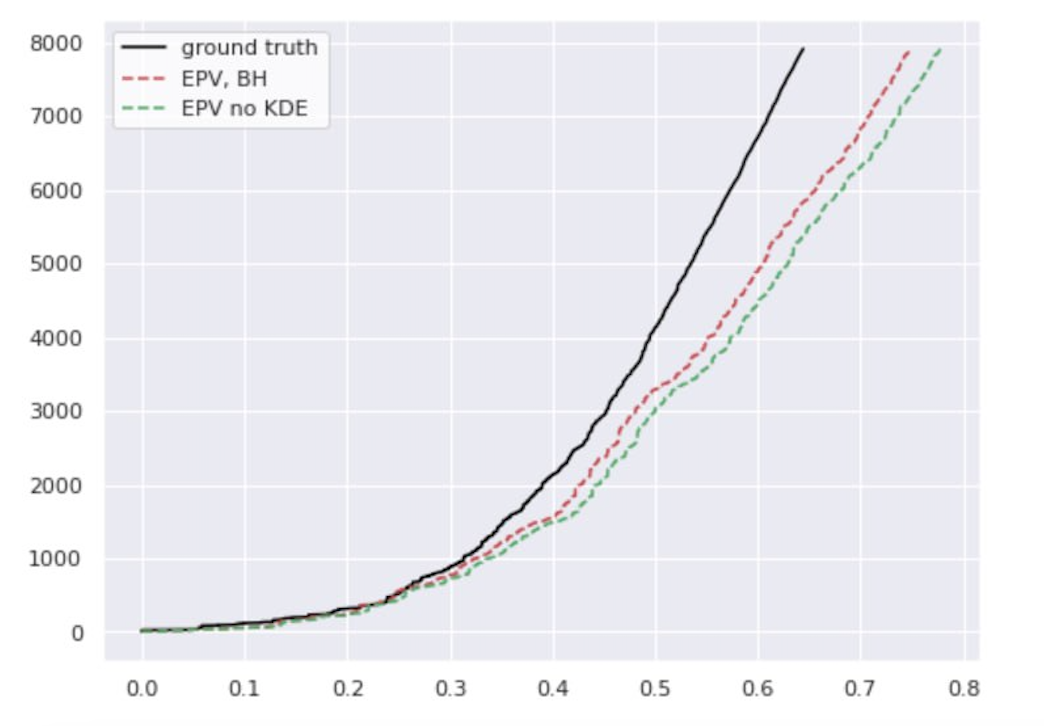
\includegraphics[width=2in]{img/tinkoff_fdr_control.png} & 
            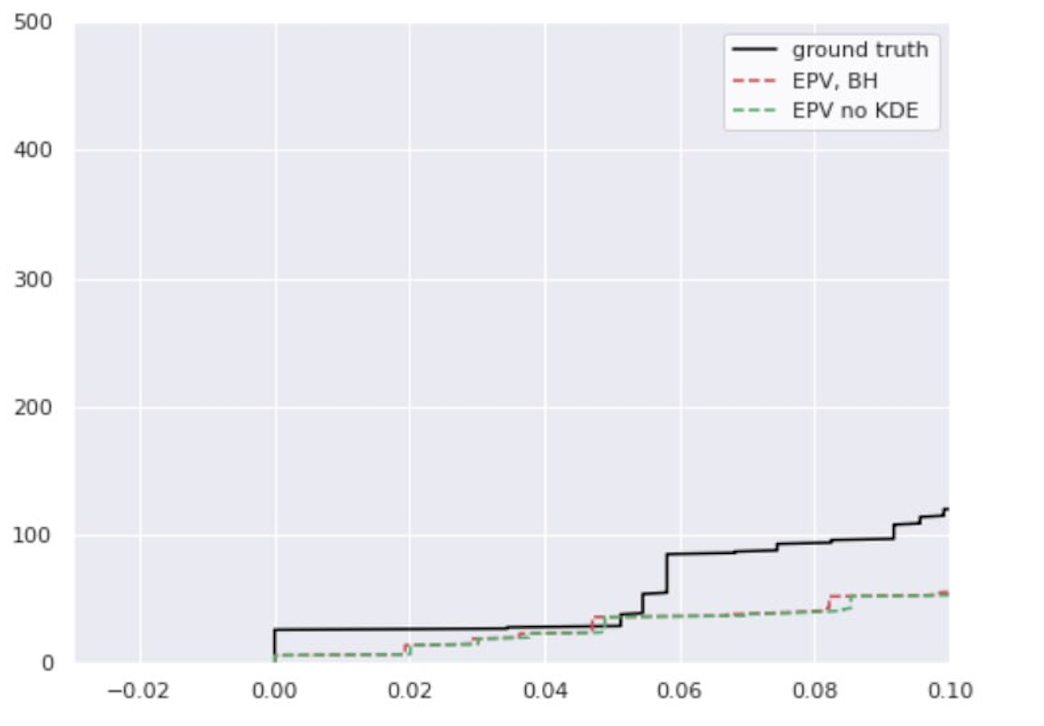
\includegraphics[width=2in]{img/tinkoff_fdr_control_loc.png}
		\\	
		A & B & C
	\end{tabular}
	\caption{\bf FDR control with p-values for credit risk.}
	\label{fig:credit risk}
\end{figure} 

\section{Conclusions}
\todo{andrey}{rewrite conclusion, add discussion}
The original exact p-value (XPV) calculation methods for scoring tandem mass spectrometry data using a dot-product-like scoring function were introduced for low-resolution fragmentation settings almost 15 years ago. Until now, it has remained an open question whether this algorithm can be made suitable for high resolution fragmentation settings. In this article we showed a generalization of the XPV method, termed HR-XPV, which is capable of producing accurate and well calibrated exact p-values for XCorr scores obtained with scoring high resolution MS/MS data. Unfortunately, our solution can be considered rather slow, which raise questions about its practicality. However, we hope that, the ideas in HR-XPV presented might be a significant step toward the development of efficient methods for calibrating exact p-values for high resolution MS/MS data. 

\section*{Author contributions}
\ifdefined\DOUBLEBLINDREVIEW
Omitted for double-blind peer-review.
\else
AKF concieved the idea that accurate empirical p-values would be derived from training data. AB worked out the methods and carried out experiments. AKF and AB wrote the manuscript.
\fi

%\printbibliography	 
%\bibliographystyle{plain}           % Style BST file.
\bibliographystyle{unsrt}           % Style BST file.
\bibliography{bibliography}

\end{document}
